\documentclass[11pt,letterpaper]{article}
\usepackage[utf8]{inputenc}
\usepackage[T1]{fontenc}
\usepackage{lmodern}
\usepackage[spanish,es-noshorthands,es-tabla,es-nodecimaldot]{babel}
\usepackage[margin=2.3cm]{geometry}
\usepackage{graphicx,float,booktabs,longtable,tabularx,array,multirow}
\usepackage{xcolor,listings,caption,enumitem,fancyhdr,tikz}
\usepackage[hidelinks]{hyperref}
\usetikzlibrary{positioning,arrows.meta,shapes.geometric}

% ------------------------------------------------------------------
% Enlaces que el grupo debe completar antes de entregar
\newcommand{\enlaceVideo}{\textcolor{red}{[pegar aquí el enlace al video]}}
\newcommand{\enlaceDumps}{\textcolor{red}{[pegar aquí el enlace a la carpeta de dumps]}}
\newcommand{\enlaceRepositorio}{\textcolor{red}{[pegar aquí el enlace a la carpeta de scripts]}}
% ------------------------------------------------------------------

\definecolor{fondo}{RGB}{247,247,247}
\definecolor{clave}{RGB}{0,70,140}
\definecolor{comentario}{RGB}{90,120,90}
\lstdefinestyle{sql}{language=SQL, basicstyle=\ttfamily\scriptsize, keywordstyle=\color{clave}\bfseries,
  commentstyle=\color{comentario}\itshape, backgroundcolor=\color{fondo}, frame=single, rulecolor=\color{black!25},
  breaklines=true, columns=fullflexible, keepspaces=true, showstringspaces=false, numbers=left,
  numberstyle=\tiny\color{black!50}, xleftmargin=1.6em, framexleftmargin=1.4em,
  morekeywords={REFERENCES,CASCADE,RESTRICT,SERIAL,BIGSERIAL,INCLUDE,USING,BRIN,RETURNS,LANGUAGE,
  PROCEDURE,CALL,TRIGGER,EXECUTE,FUNCTION,RAISE,EXCEPTION,NOTICE,RETURNING,FILTER,OVER,PARTITION,
  RANK,WITH,RECURSIVE,LATERAL,CONFLICT,NOTHING,COMMENT,INTERVAL,EXPLAIN,ANALYZE,VACUUM,BOOLEAN,
  TIMESTAMP,SMALLINT,NUMERIC,COALESCE,NULLIF,EXISTS,DISTINCT,ROUND,BEGIN,END,DECLARE,ELSIF,
  PERFORM,FOUND,NEW,OLD,DO,IF,THEN,ELSE,RETURN,REPLACE,VIEW,GRANT,REVOKE,ROLE}}
\lstdefinestyle{plano}{basicstyle=\ttfamily\tiny, backgroundcolor=\color{fondo}, frame=single, breakautoindent=false,
  rulecolor=\color{black!25}, breaklines=true, columns=fullflexible, keepspaces=true}
\lstdefinestyle{py}{language=Python, basicstyle=\ttfamily\tiny, keywordstyle=\color{clave}\bfseries,
  commentstyle=\color{comentario}\itshape, stringstyle=\color{black!70}, backgroundcolor=\color{fondo},
  frame=single, rulecolor=\color{black!25}, breaklines=true, columns=fullflexible, keepspaces=true,
  showstringspaces=false}
\lstset{style=sql, literate={á}{{\'a}}1 {é}{{\'e}}1 {í}{{\'i}}1 {ó}{{\'o}}1 {ú}{{\'u}}1 {ñ}{{\~n}}1
  {Á}{{\'A}}1 {É}{{\'E}}1 {Í}{{\'I}}1 {Ó}{{\'O}}1 {Ú}{{\'U}}1 {Ñ}{{\~N}}1 {°}{{$^\circ$}}1}

\newcommand{\tbus}{\textunderscore\allowbreak}
\newcommand{\tb}[1]{{\ttfamily\let\_\tbus #1}}
\newcommand{\pk}[1]{\underline{#1}}
\newcommand{\fk}[2]{{\itshape\let\_\tbus #1}$^{\to\,\textsc{\let\_\tbus #2}}$}
\setlength{\parskip}{0.45em}
\setlength{\emergencystretch}{3em}
\setlength{\parindent}{0pt}
\renewcommand{\arraystretch}{1.12}
\captionsetup{font=small,labelfont=bf}
\pagestyle{fancy}\fancyhf{}
\lhead{\small CS2041 Base de Datos I}\rhead{\small Agricultura de precisión e IoT}
\cfoot{\small\thepage}

\begin{document}

% ================================================================== PORTADA
\begin{titlepage}
\centering
{\large UNIVERSIDAD DE INGENIERÍA Y TECNOLOGÍA\par}
\vspace{0.3cm}
{\large UTEC\par}
\vspace{2.2cm}
{\normalsize Curso: Base de Datos I (CS2041), Laboratorio 14\par}
\vspace{0.3cm}
{\normalsize Ciclo 2026-2\par}
\vspace{2cm}
{\LARGE\bfseries Proyecto final\par}
\vspace{0.4cm}
{\Large Agricultura de Precisión y Sensores IoT Agropecuarios\par}
\vspace{2.4cm}
{\large Integrantes\par}
\vspace{0.3cm}
Lescano Garamendi, Juan Carlos Sebastián : 202510447\par
Rojas Meza, Kiara Luz : 202510620\par
\vspace{1.6cm}
{\large Profesor\par}
\vspace{0.3cm}
Ojeda Rios, Brenner Humberto\par
\vfill
{\normalsize Lima, Perú\par}
\end{titlepage}

\tableofcontents
\newpage

% ================================================================== 1
\section{Requisitos}

\subsection{Introducción}

La agricultura de precisión parte de una idea sencilla: un campo no es homogéneo. Dos sectores de la misma parcela pueden tener suelos, pendientes y capacidades de retención de agua distintas, así que regarlos y fertilizarlos por igual desperdicia agua en uno y estresa al cultivo en el otro. Para manejar cada sector por separado hace falta medir, y hoy esa medición la hacen sensores de suelo conectados por radio que reportan humedad, temperatura, conductividad eléctrica y pH varias veces por hora.

En la costa peruana el agua es el recurso que limita la producción. Los fundos agroexportadores de Ica, La Libertad o Piura riegan con agua de pozo o de canal, pagan por ella y deben justificar su uso ante la Autoridad Nacional del Agua. En ese contexto, saber cuántos litros cuesta producir un kilogramo de espárrago o de arándano deja de ser un dato académico y se vuelve un indicador de gestión.

Este proyecto diseña e implementa la base de datos de una empresa agroexportadora que ya instaló sensores y controladores de riego en sus fundos, pero que guarda la información en lugares desconectados entre sí. Construimos el modelo conceptual, el modelo relacional y el modelo físico en PostgreSQL 16, poblamos la base con datos sintéticos en cuatro volúmenes (mil, diez mil, cien mil y un millón de registros) y medimos el efecto de distintos índices sobre cinco consultas de nivel intermedio.

\subsection{Descripción general del problema y de la organización}

El caso de estudio es Agroandina del Pacífico S.A.C.\footnote{Nombre ficticio. El caso se construyó con información pública del sector agroexportador peruano y con fichas técnicas de sensores comerciales.}, una empresa con 12 fundos repartidos en 12 departamentos del país. En la costa produce espárrago, arándano, palta Hass, uva de mesa, mango, alcachofa y pimiento piquillo; en Arequipa, quinua y papa; y en la selva alta, café y cacao. Maneja 600 parcelas que suman cerca de 10\,553 hectáreas, divididas en 2\,400 zonas de manejo.

La empresa tiene instalados 2\,200 sensores de suelo y 600 controladores de válvulas. Los sensores provienen de varios fabricantes y cada uno envía sus datos a una plataforma web propia. Los controladores registran los riegos en la consola del proveedor del sistema. Las cosechas se anotan en hojas de cálculo por fundo y las aplicaciones de fertilizantes y plaguicidas se escriben en cuadernos de campo que un asistente transcribe cada semana.

El problema concreto es que ninguna de estas fuentes comparte un identificador común. Un sensor se reconoce por su número de serie, una parcela por un código interno que cambia de un fundo a otro y una cosecha por la fecha y el nombre del supervisor. Cruzar los riegos de una parcela con lo que esa parcela produjo toma días de trabajo manual y el resultado suele tener errores.

\subsection{Necesidad y usos de la base de datos}

La gerencia agrícola necesita un repositorio único que permita responder preguntas que hoy no puede contestar a tiempo:

\begin{itemize}[leftmargin=1.4em,itemsep=0.1em]
\item Qué parcelas están por debajo de la humedad mínima que su cultivo tolera y desde cuándo.
\item Cuánta agua consume cada campaña por kilogramo cosechado, dato que además pide la certificación GLOBALG.A.P. y que sirve para renovar licencias de uso de agua.
\item Qué sensores reportan valores anómalos con demasiada frecuencia, lo que suele indicar un equipo descalibrado antes que un problema del suelo.
\item Qué parcelas rinden más dentro de cada fundo y con qué cultivo.
\item Si el personal de riego reacciona a las alertas de humedad crítica dentro de un plazo razonable.
\end{itemize}

También se requiere trazabilidad: para exportar hay que demostrar qué producto se aplicó en qué zona, quién lo aplicó y que se respetó el periodo de carencia antes de cosechar.

\subsection{¿Cómo se resuelve el problema hoy?}

\subsubsection{¿Cómo se almacenan y procesan los datos hoy?}

Hoy cada tipo de dato vive en un sistema distinto. Las lecturas de los sensores se descargan como archivos CSV desde los portales de los fabricantes, con columnas y formatos de fecha diferentes según la marca. Los riegos se exportan desde la consola de los controladores. Las cosechas están en un libro de Excel por fundo, con una hoja por campaña. Los cuadernos de aplicación se transcriben a otro Excel compartido y los avisos de humedad baja llegan por un grupo de WhatsApp en el que participan los operadores de riego.

Un analista une estos archivos a mano una vez por semana. Como no hay claves comunes, el cruce se hace por nombres y fechas aproximadas, lo que produce duplicados cuando un mismo sensor se reinstala en otra zona y omisiones cuando un supervisor escribe mal el código de la parcela.

\subsubsection{Flujo de datos}

La Figura~\ref{fig:flujo_actual} resume el flujo actual. La información pasa por al menos tres transcripciones antes de llegar a quien decide, y el ciclo completo tarda una semana.

\begin{figure}[H]
\centering
\begin{tikzpicture}[node distance=0.45cm and 0.55cm, every node/.style={font=\scriptsize, align=center},
  caja/.style={draw, rounded corners=2pt, minimum height=0.9cm, text width=2.05cm, fill=black!4},
  flecha/.style={-{Stealth[length=2mm]}, thick}]
\node[caja] (s) {Sensores de\\suelo};
\node[caja, right=of s] (p) {Portales de\\fabricantes};
\node[caja, right=of p] (c) {Archivos CSV\\por marca};
\node[caja, right=of c] (e) {Excel consolidado\\(semanal)};
\node[caja, right=of e] (g) {Reporte a\\gerencia};
\node[caja, below=of p] (r) {Consola de\\controladores};
\node[caja, below=of e] (k) {Cuadernos y\\Excel de cosecha};
\node[caja, below=of s] (w) {Avisos por\\WhatsApp};
\draw[flecha] (s) -- (p); \draw[flecha] (p) -- (c); \draw[flecha] (c) -- (e); \draw[flecha] (e) -- (g);
\draw[flecha] (r) -| (e); \draw[flecha] (k) -- (e); \draw[flecha, dashed] (s) -- (w);
\end{tikzpicture}
\caption{Flujo de datos actual.}
\label{fig:flujo_actual}
\end{figure}

Con la base de datos propuesta el flujo cambia (Figura~\ref{fig:flujo_nuevo}). Un servicio de ingesta recibe los mensajes del gateway LoRaWAN y llama al procedimiento \tb{sp\_registrar\_lectura}. Al insertarse la lectura, un trigger evalúa si la humedad está por debajo del mínimo del cultivo vigente y, si es así, crea la alerta. Los controladores registran cada riego en \tb{Evento\_Riego}, los supervisores registran cosechas y aplicaciones desde el campo, y la gerencia consulta vistas que ya traen los indicadores calculados.

\begin{figure}[H]
\centering
\begin{tikzpicture}[node distance=0.45cm and 0.5cm, every node/.style={font=\scriptsize, align=center},
  caja/.style={draw, rounded corners=2pt, minimum height=0.9cm, text width=2.05cm, fill=black!4},
  bd/.style={draw, cylinder, shape border rotate=90, aspect=0.18, minimum height=1.6cm, text width=2.3cm, fill=blue!6},
  flecha/.style={-{Stealth[length=2mm]}, thick}]
\node[caja] (s) {Sensores y\\controladores};
\node[caja, right=of s] (g) {Gateway\\LoRaWAN};
\node[caja, right=of g] (i) {Servicio de ingesta\\(procedimientos)};
\node[bd, right=of i] (b) {PostgreSQL\\tablas, triggers\\y vistas};
\node[caja, right=of b] (u) {Gerencia,\\agrónomos y\\operarios};
\node[caja, below=of i] (m) {Registro en campo\\(cosecha, insumos)};
\draw[flecha] (s) -- (g); \draw[flecha] (g) -- (i); \draw[flecha] (i) -- (b); \draw[flecha] (b) -- (u);
\draw[flecha] (m) -| (b);
\end{tikzpicture}
\caption{Flujo de datos con la base de datos propuesta.}
\label{fig:flujo_nuevo}
\end{figure}

\subsection{Descripción detallada del sistema}

\subsubsection{Objetos de información actuales}

Los objetos de información que la empresa ya maneja, aunque dispersos, son los siguientes:

\begin{itemize}[leftmargin=1.4em,itemsep=0.1em]
\item \textbf{Fundos y parcelas.} Nombre, ubicación política, coordenadas, área, tipo de suelo y pendiente. Cambian muy poco.
\item \textbf{Zonas de manejo.} Sectores de riego dentro de cada parcela. Se redefinen cuando se rediseña el sistema de riego.
\item \textbf{Catálogo de cultivos.} Rangos óptimos de humedad, pH y conductividad, y duración del ciclo. Se toman de fichas técnicas y de la guía FAO-56 de evapotranspiración.
\item \textbf{Campañas.} Qué cultivo se sembró en qué parcela y entre qué fechas.
\item \textbf{Dispositivos.} Número de serie, modelo, fabricante, fecha de instalación y zona. Los sensores añaden tipo y profundidad; los controladores, el sistema de riego que accionan y el caudal de la válvula.
\item \textbf{Lecturas de suelo.} Humedad volumétrica, temperatura, pH, conductividad y batería, con marca de tiempo. Es el objeto más voluminoso: un sensor que reporta cada 15 minutos genera 96 lecturas diarias.
\item \textbf{Riegos, alertas, cosechas, aplicaciones de insumos y mantenimientos}, cada uno con su fecha, su responsable y sus cantidades.
\end{itemize}

\subsubsection{Características y funcionalidades esperadas}

Se espera un repositorio central en el que cada lectura, riego y cosecha quede asociado sin ambigüedad a una zona, una parcela y una campaña. Las reglas del negocio deben vivir en la base de datos y no en la buena voluntad de quien digita: rangos válidos, fechas coherentes, campañas que no se superpongan, alertas que se generen solas y un rendimiento por hectárea que se actualice con cada cosecha.

En cuanto a desempeño, las consultas operativas (alertas pendientes, estado hídrico de una zona) deben responder en menos de un segundo, y los reportes analíticos sobre toda la serie, en pocos segundos. La carga masiva de datos históricos debe poder hacerse en minutos.

\subsubsection{Tipos de usuarios existentes y necesarios}

La Tabla~\ref{tab:usuarios} resume los perfiles y lo que cada uno puede hacer. El script opcional \tb{05\_roles.sql} crea estos roles en PostgreSQL con los permisos indicados.

\begin{table}[H]
\centering\small
\begin{tabularx}{\textwidth}{>{\raggedright\arraybackslash}p{3.1cm}X}
\toprule
\textbf{Perfil} & \textbf{Acceso} \\
\midrule
Gerencia agrícola & Solo lectura sobre las vistas de producción, eficiencia hídrica y alertas. No ve datos personales de los operarios. \\
Ingeniero agrónomo & Lectura de todo el esquema. Crea y cierra campañas, mantiene el catálogo de cultivos e insumos. \\
Operador de riego & Registra eventos de riego y marca alertas como atendidas. Consulta lecturas y el estado hídrico. \\
Técnico de campo & Registra aplicaciones de insumos, cosechas y mantenimientos de equipos. \\
Plataforma IoT & Cuenta de servicio. Solo puede ejecutar \tb{sp\_registrar\_lectura}; no tiene acceso directo a las tablas. \\
Administrador de BD & Control total: estructura, respaldos, índices y usuarios. \\
\bottomrule
\end{tabularx}
\caption{Perfiles de usuario.}
\label{tab:usuarios}
\end{table}

\subsubsection{Tipos de consulta y actualizaciones}

Las consultas más frecuentes son de tres tipos. Las operativas buscan pocas filas recientes: la última lectura de una zona, las alertas sin atender o los riegos de hoy. Las de seguimiento agregan un periodo corto, por ejemplo la humedad promedio del último mes por parcela. Las analíticas recorren toda la historia: eficiencia hídrica por campaña, ranking de rendimiento o proporción de lecturas anómalas por sensor. Las cinco consultas del experimento (Sección~\ref{sec:consultas}) cubren estos tres tipos.

Las actualizaciones tienen ritmos muy distintos, como muestra la Tabla~\ref{tab:ritmos}.

\begin{table}[H]
\centering\small
\begin{tabularx}{\textwidth}{>{\raggedright\arraybackslash}p{3.3cm}>{\raggedright\arraybackslash}p{3.2cm}X}
\toprule
\textbf{Dato} & \textbf{Frecuencia} & \textbf{Forma de carga} \\
\midrule
Lecturas de suelo & Cada 5 a 60 min por sensor & Inserción continua vía procedimiento; nunca se modifican. \\
Alertas & Según las lecturas & Las crea un trigger; el operador solo actualiza la atención. \\
Eventos de riego & Varias veces al día & Inserción automática desde el controlador o manual. \\
Cosechas & Diaria en temporada & Inserción por el supervisor; recalcula el rendimiento. \\
Aplicaciones de insumos & Semanal & Inserción por el técnico de campo. \\
Campañas & Por temporada & Alta y cambio de estado por el agrónomo (auditado). \\
Fundos, parcelas, cultivos & Rara vez & Carga inicial y ajustes puntuales. \\
\bottomrule
\end{tabularx}
\caption{Ritmo de carga y modificación de los datos.}
\label{tab:ritmos}
\end{table}

\subsubsection{Tamaño estimado de la base de datos}

El escenario de un millón de registros ocupa 170.2~MB en disco con todos sus índices. La tabla \tb{Lectura\_Suelo} concentra el 77.0~\% del espacio ocupado por las tablas (Tabla~\ref{tab:tamanos}). Cada lectura ocupa en promedio 171 bytes entre datos e índices.

\begin{table}[H]
\centering\small
\begin{tabular}{lrrrr}
\toprule
Tabla & Filas & Datos (MB) & Índices (MB) & Total (MB) \\
\midrule
Lectura\_Suelo & 765\,861 & 49.0 & 75.7 & 124.8 \\
Evento\_Riego & 120\,000 & 9.7 & 9.9 & 19.6 \\
Alerta & 30\,000 & 2.8 & 3.1 & 5.9 \\
Cosecha & 25\,000 & 1.8 & 2.6 & 4.4 \\
Aplicacion\_Insumo & 40\,000 & 2.7 & 1.6 & 4.3 \\
Mantenimiento & 8\,000 & 0.7 & 0.3 & 1.0 \\
Dispositivo & 2\,800 & 0.2 & 0.3 & 0.5 \\
Campania & 1\,500 & 0.1 & 0.2 & 0.3 \\
Otras 10 tablas & 6\,839 & 0.5 & 0.4 & 1.2 \\
\textbf{Total} &  &  &  & \textbf{161.9} \\
\bottomrule
\end{tabular}
\caption{Espacio ocupado por tabla en el escenario de un millón.}\label{tab:tamanos}
\end{table}


Ese millón de registros es, sin embargo, una muestra. Si los 2\,200 sensores reportaran realmente cada 15 minutos, la empresa generaría unos 77.1 millones de lecturas al año, es decir, alrededor de 13.2 GB anuales solo en esa tabla con el esquema de índices actual. Ese orden de magnitud condiciona las decisiones de la Sección~\ref{sec:extra}.

\subsection{Objetivos del proyecto}

El objetivo general es diseñar e implementar en PostgreSQL una base de datos que integre la información de sensores, riego, campañas y cosechas de la empresa, y evaluar experimentalmente cómo responde a volúmenes crecientes de datos.

Los objetivos específicos son:
\begin{enumerate}[leftmargin=1.6em,itemsep=0.1em]
\item Modelar el dominio con una jerarquía Is-A, entidades débiles y una relación ternaria, y transformarlo a un esquema relacional en tercera forma normal.
\item Trasladar las reglas del negocio a restricciones, procedimientos y triggers para que la base de datos las haga cumplir por sí misma.
\item Generar datos sintéticos coherentes con la realidad agronómica peruana en cuatro volúmenes.
\item Medir cinco consultas intermedias con y sin índices, comparar tipos de índice y cuantificar cuánto encarecen los índices las operaciones de escritura.
\item Proponer una estrategia de crecimiento para volúmenes superiores al millón de registros.
\end{enumerate}

\subsection{Referencias del proyecto}

Los rangos óptimos por cultivo y la relación entre humedad del suelo y estrés hídrico se tomaron de la guía FAO-56 y de fichas técnicas públicas. Los modelos de sensores y controladores corresponden a equipos comerciales reales, pero sus datos son simulados. Para el diseño y la implementación seguimos la bibliografía del curso y la documentación oficial de PostgreSQL.

\begin{itemize}[leftmargin=1.4em,itemsep=0.1em]
\item Allen, R., Pereira, L., Raes, D. y Smith, M. (1998). \textit{Crop evapotranspiration: guidelines for computing crop water requirements}. FAO Irrigation and Drainage Paper 56.
\item Garcia-Molina, H., Ullman, J. y Widom, J. (2009). \textit{Database Systems: The Complete Book} (2.ª ed.). Pearson.
\item Elmasri, R. y Navathe, S. (2016). \textit{Fundamentals of Database Systems} (7.ª ed.). Pearson.
\item PostgreSQL Global Development Group. \textit{PostgreSQL 16 Documentation}. \url{https://www.postgresql.org/docs/16/}
\item Autoridad Nacional del Agua. \url{https://www.gob.pe/ana}
\item Ministerio de Desarrollo Agrario y Riego. \url{https://www.gob.pe/midagri}
\item GLOBALG.A.P. Integrated Farm Assurance Standard. \url{https://www.globalgap.org}
\item METER Group. Ficha técnica del sensor TEROS 12. \url{https://www.metergroup.com}
\end{itemize}

\subsection{Eventualidades}

\subsubsection{Problemas que pudieran encontrarse en el proyecto}

El primer problema es el acceso a datos reales. Las lecturas de sensores de una empresa privada son información comercial y no están publicadas, por eso trabajamos con datos sintéticos construidos con parámetros reales. El riesgo es que la simulación no reproduzca fenómenos que sí ocurren en campo, como la deriva gradual de un sensor o la estacionalidad de la humedad entre invierno y verano.

Otros problemas previsibles son técnicos. Los sensores pueden enviar dos lecturas con la misma marca de tiempo si su reloj se desfasa, lo que chocaría con la clave primaria; por eso el procedimiento de registro ignora duplicados con \tb{ON CONFLICT DO NOTHING}. También hay pérdidas de transmisión que dejan huecos en las series, y cambios de formato cuando un proveedor actualiza su plataforma. Por último, todas las mediciones se hicieron en una sola máquina, así que los tiempos absolutos dependen de ese equipo; lo que se puede comparar con confianza son las proporciones entre escenarios y entre configuraciones.

\subsubsection{Límites y alcances del proyecto}

El proyecto cubre el modelo conceptual, el relacional y el físico, la carga de datos en cuatro volúmenes, las vistas, procedimientos y triggers, y el experimento de optimización con sus variantes. No incluye el servicio de ingesta en tiempo real ni una aplicación web, tampoco datos meteorológicos o imágenes satelitales, ni algoritmos de recomendación de riego. Estos elementos se mencionan como trabajo futuro porque el esquema está preparado para recibirlos.

% ================================================================== 2
\section{Modelo Entidad-Relación}

\subsection{Reglas semánticas}

Cada regla indica entre paréntesis el mecanismo que la hace cumplir en la implementación. Las multiplicidades se expresan como mínimo y máximo de participación.

\begin{enumerate}[label=\textbf{R\arabic*.},leftmargin=2.3em,itemsep=0.15em]
\item Un fundo tiene una o más parcelas y cada parcela pertenece a exactamente un fundo. El código de la parcela se repite entre fundos, pero no dentro del mismo fundo (FK, \tb{NOT NULL}, \tb{UNIQUE}).
\item Cada parcela se divide en una o más zonas de manejo. Una zona no existe fuera de su parcela y se identifica por su número dentro de ella: es una entidad débil (PK compuesta, \tb{ON DELETE CASCADE}).
\item Un cultivo puede sembrarse en muchas campañas y una parcela puede tener muchas campañas a lo largo del tiempo; cada campaña corresponde a exactamente una parcela y a exactamente un cultivo (FK, \tb{NOT NULL}).
\item En una misma parcela, dos campañas no pueden superponerse en el tiempo. En consecuencia, en una fecha dada hay a lo sumo una campaña en curso por parcela (trigger \tb{trg\_campania\_sin\_solape}).
\item La fecha de fin estimada de una campaña es posterior a su fecha de siembra (\tb{CHECK}).
\item Una parcela puede tener cero o más sistemas de riego; las parcelas de secano de la selva no tienen ninguno. Cada sistema abastece a una sola parcela (FK).
\item Todo dispositivo está instalado en exactamente una zona de manejo; una zona puede tener cero o más dispositivos (FK compuesta).
\item Todo dispositivo es un sensor o un controlador, y nunca ambos a la vez. La especialización es total y disjunta (trigger \tb{trg\_fn\_subclase\_exclusiva} y procedimiento \tb{sp\_registrar\_dispositivo}).
\item Cada controlador acciona exactamente un sistema de riego, que debe ser el de la parcela donde está instalado (FK y verificación de carga).
\item Un sensor emite cero o más lecturas y cada lectura pertenece a un solo sensor. La lectura se identifica por el minuto en que se tomó dentro de ese sensor: es una entidad débil y un sensor no puede reportar dos veces en el mismo minuto (PK compuesta).
\item Las variables presentes en una lectura dependen del tipo de sensor. Un sensor de pH no mide humedad y uno de temperatura solo mide temperatura; en esos casos la columna queda nula por diseño.
\item Toda alerta se origina en exactamente una lectura, y una lectura origina a lo sumo una alerta de cada tipo (FK compuesta hacia la lectura, \tb{UNIQUE}).
\item Si la humedad de una lectura cae por debajo del mínimo del cultivo en curso, o la batería baja de 15~\%, se genera la alerta correspondiente sin intervención humana (trigger \tb{trg\_alerta\_lectura}).
\item Una alerta atendida debe tener fecha de atención, y una no atendida no puede tenerla (\tb{CHECK}).
\item Un evento de riego usa exactamente un sistema sobre exactamente una zona, y esa zona debe pertenecer a la parcela que abastece el sistema. Puede tener un operario responsable o ninguno si fue automático (FK y trigger \tb{trg\_evento\_riego}).
\item En una zona no pueden empezar dos riegos en el mismo minuto (\tb{UNIQUE}).
\item Si el controlador no informa el volumen aplicado, este se calcula como caudal nominal por duración (trigger \tb{trg\_evento\_riego}).
\item Una campaña tiene cero o más registros de cosecha y cada cosecha pertenece a una sola campaña. Las campañas perdidas no registran cosecha (FK y verificación de carga).
\item El rendimiento de una campaña es un atributo derivado: kilogramos cosechados entre el área de la parcela (trigger \tb{trg\_rendimiento}).
\item En una aplicación de insumo intervienen exactamente una zona, un insumo y un operario en un instante dado. La misma terna puede repetirse en otro momento, pero no en el mismo (relación ternaria, PK de cinco columnas).
\item Un operario puede dar mantenimiento a muchos dispositivos y un dispositivo puede ser atendido por muchos operarios. Un operario no registra dos mantenimientos del mismo equipo en la misma fecha (relación N:M, PK compuesta).
\item Todo operario tiene un DNI de ocho dígitos que no se repite, y su teléfono, si existe, tiene nueve dígitos (\tb{UNIQUE}, \tb{CHECK} con expresión regular).
\item Los valores medidos respetan rangos físicos: humedad entre 0 y 100~\%, pH entre 0 y 14, conductividad no negativa, temperatura entre $-10$ y 60~°C (\tb{CHECK}).
\item Todo cambio de estado de una campaña queda registrado con usuario y fecha (trigger \tb{trg\_auditoria\_campania}).
\end{enumerate}

\subsection{Modelo Entidad-Relación}

La Figura~\ref{fig:er} presenta el diagrama. Usamos notación de Chen: rectángulos para entidades, óvalos para atributos, rombos para relaciones y triángulos para la especialización. Las claves se subrayan con línea continua y las claves parciales de las entidades débiles, con línea discontinua. Siguiendo a Garcia-Molina, Ullman y Widom, una flecha que llega a una entidad indica que cada instancia del otro lado se relaciona con a lo sumo una instancia de ella. Siguiendo a Elmasri y Navathe, la línea doble indica participación total. Las entidades débiles y sus relaciones identificadoras se dibujan con borde doble y el atributo derivado, con óvalo punteado.

\begin{figure}[H]
\centering
\IfFileExists{figuras/diagrama_er.png}{%
  \includegraphics[width=\textwidth]{figuras/diagrama_er.png}}{%
  \fbox{\parbox[c][7cm][c]{0.9\textwidth}{\centering\textcolor{red}{Insertar aquí el diagrama exportado desde Lucid\\como \tb{informe/figuras/diagrama\_er.png}}}}}
\caption{Modelo entidad-relación.}
\label{fig:er}
\end{figure}

\subsection{Especificaciones y consideraciones sobre el modelo}

\textbf{Campaña como entidad.} Una campaña podría verse como la relación \emph{se siembra} entre \tb{Parcela} y \tb{Cultivo}. La modelamos como entidad porque tiene identidad propia, porque la misma parcela repite el mismo cultivo en años distintos y porque otras entidades dependen de ella: las cosechas se registran contra una campaña concreta, no contra un par parcela-cultivo.

\textbf{Dos entidades débiles.} \tb{Zona\_Manejo} depende de \tb{Parcela}: la zona 3 solo tiene sentido dentro de su parcela. \tb{Lectura\_Suelo} depende de \tb{Sensor}: una medición aislada del equipo que la tomó no significa nada, y el instante basta para distinguirla dentro de ese equipo. Tratar la lectura como débil evita además un identificador artificial en la tabla más grande del esquema, lo que ahorra espacio y un índice.

\textbf{Especialización total y disjunta.} \tb{Dispositivo} generaliza a \tb{Sensor} y \tb{Controlador}. Es total porque la empresa no instala equipos que no sean de uno de los dos tipos, y disjunta porque un nodo que mide y a la vez acciona válvulas se registra como dos dispositivos. Cada subclase tiene atributos y relaciones propias: solo los sensores emiten lecturas y solo los controladores accionan un sistema de riego.

\textbf{Relación ternaria.} \tb{Aplica} relaciona \tb{Zona\_Manejo}, \tb{Insumo} y \tb{Operario}. No se puede reemplazar por tres relaciones binarias sin perder información: saber qué operario aplicó qué insumo y en qué zona trabajó cada operario no permite reconstruir quién aplicó qué cosa dónde. La terna es de muchos a muchos a muchos, por eso ninguno de sus arcos lleva flecha.

\textbf{Atributos compuestos y derivados.} La ubicación del fundo (departamento, provincia, distrito) y los rangos óptimos del cultivo (mínimo y máximo de humedad y de pH) son atributos compuestos que se aplanan en columnas simples. El rendimiento por hectárea de la campaña es derivado; se almacena por rendimiento de consulta y lo mantiene un trigger.

\textbf{Tabla fuera del modelo conceptual.} \tb{Auditoria\_Campania} es una bitácora técnica alimentada por un trigger. No representa un objeto del negocio, por lo que no aparece en el diagrama.

\textbf{Relaciones del diagrama.} Además de las ya descritas, el modelo incluye: \emph{tiene} (Fundo--Parcela), \emph{se divide en} (Parcela--Zona, identificadora), \emph{se siembra en} (Campaña--Parcela), \emph{corresponde a} (Campaña--Cultivo), \emph{labora en} (Operario--Fundo), \emph{abastece} (Sistema--Parcela), \emph{instalado en} (Dispositivo--Zona), \emph{acciona} (Controlador--Sistema), \emph{registra} (Sensor--Lectura, identificadora), \emph{origina} (Lectura--Alerta), \emph{atiende} (Operario--Alerta), \emph{ejecuta} (Sistema--Evento), \emph{riega} (Evento--Zona), \emph{opera} (Operario--Evento), \emph{produce} (Campaña--Cosecha), \emph{recoge} (Operario--Cosecha) y \emph{mantiene} (Operario--Dispositivo, N:M). En total el modelo tiene 15 entidades, contando las dos subclases, y 18 relaciones.

% ================================================================== 3
\section{Modelo Relacional}

\subsection{Modelo Relacional}

El esquema tiene 18 relaciones: 15 provienen de las entidades del modelo conceptual, dos implementan relaciones con atributos propios (\tb{Aplicacion\_Insumo} y \tb{Mantenimiento}) y una es la bitácora técnica \tb{Auditoria\_Campania}. Las claves primarias van subrayadas y las claves foráneas en cursiva, con una flecha hacia la tabla referenciada. La lista se generó desde el catálogo de PostgreSQL, por lo que coincide exactamente con lo implementado.

\begin{itemize}[leftmargin=1.2em,itemsep=0.3em]
\item \textsc{Fundo}(\pk{id\_fundo}, nombre, departamento, provincia, distrito, area\_total\_ha, latitud, longitud, fecha\_registro)
\item \textsc{Parcela}(\pk{id\_parcela}, \fk{id\_fundo}{Fundo}, codigo\_parcela, area\_ha, tipo\_suelo, pendiente\_pct, fecha\_habilitacion)
\item \textsc{Zona\_Manejo}(\pk{\fk{id\_parcela}{Parcela}}, \pk{num\_zona}, area\_ha, descripcion)
\item \textsc{Cultivo}(\pk{id\_cultivo}, nombre\_comun, nombre\_cientifico, ciclo\_dias, humedad\_optima\_min, humedad\_optima\_max, ph\_optimo\_min, ph\_optimo\_max, ce\_maxima\_ds\_m)
\item \textsc{Operario}(\pk{id\_operario}, dni, nombre, apellido, rol, telefono, \fk{id\_fundo}{Fundo}, fecha\_ingreso)
\item \textsc{Campania}(\pk{id\_campania}, \fk{id\_parcela}{Parcela}, \fk{id\_cultivo}{Cultivo}, fecha\_siembra, fecha\_fin\_estimada, densidad\_plantas\_ha, estado, rendimiento\_kg\_ha)
\item \textsc{Sistema\_Riego}(\pk{id\_sistema}, \fk{id\_parcela}{Parcela}, tipo, caudal\_nominal\_lph, fuente\_agua, fecha\_instalacion, estado)
\item \textsc{Dispositivo}(\pk{id\_dispositivo}, codigo\_serie, modelo, fabricante, fecha\_instalacion, estado, \fk{id\_parcela}{Zona\_Manejo}, \fk{num\_zona}{Zona\_Manejo})
\item \textsc{Sensor}(\pk{\fk{id\_dispositivo}{Dispositivo}}, tipo\_sensor, profundidad\_cm, frecuencia\_min, unidad\_medida, rango\_min, rango\_max)
\item \textsc{Controlador}(\pk{\fk{id\_dispositivo}{Dispositivo}}, \fk{id\_sistema}{Sistema\_Riego}, caudal\_max\_lps, tipo\_valvula)
\item \textsc{Lectura\_Suelo}(\pk{\fk{id\_dispositivo}{Sensor}}, \pk{fecha\_hora}, humedad\_pct, temperatura\_c, ph, conductividad\_ds\_m, bateria\_pct)
\item \textsc{Evento\_Riego}(\pk{id\_evento}, \fk{id\_sistema}{Sistema\_Riego}, \fk{id\_parcela}{Zona\_Manejo}, \fk{num\_zona}{Zona\_Manejo}, \fk{id\_operario}{Operario}, fecha\_hora\_inicio, duracion\_min, volumen\_litros, modo)
\item \textsc{Alerta}(\pk{id\_alerta}, \fk{id\_dispositivo}{Lectura\_Suelo}, \fk{fecha\_hora}{Lectura\_Suelo}, tipo, severidad, valor\_registrado, atendida, fecha\_atencion, \fk{id\_operario}{Operario})
\item \textsc{Cosecha}(\pk{id\_cosecha}, \fk{id\_campania}{Campania}, \fk{id\_operario}{Operario}, fecha, cantidad\_kg, categoria, humedad\_producto\_pct, precio\_kg\_soles)
\item \textsc{Insumo}(\pk{id\_insumo}, nombre, tipo, unidad, costo\_unitario, periodo\_carencia\_dias)
\item \textsc{Aplicacion\_Insumo}(\pk{\fk{id\_parcela}{Zona\_Manejo}}, \pk{\fk{num\_zona}{Zona\_Manejo}}, \pk{\fk{id\_insumo}{Insumo}}, \pk{\fk{id\_operario}{Operario}}, \pk{fecha\_hora}, dosis, metodo)
\item \textsc{Mantenimiento}(\pk{\fk{id\_dispositivo}{Dispositivo}}, \pk{\fk{id\_operario}{Operario}}, \pk{fecha}, tipo, observacion, costo)
\item \textsc{Auditoria\_Campania}(\pk{id\_auditoria}, id\_campania, estado\_anterior, estado\_nuevo, usuario\_bd, fecha\_cambio)
\end{itemize}

\subsection{Especificaciones de transformación}

\subsubsection{Entidades}

Cada entidad fuerte se convirtió en una tabla con sus atributos simples: \tb{Fundo}, \tb{Parcela}, \tb{Cultivo}, \tb{Operario}, \tb{Campania}, \tb{Sistema\_Riego}, \tb{Dispositivo}, \tb{Evento\_Riego}, \tb{Alerta}, \tb{Cosecha} e \tb{Insumo}. Los atributos compuestos se aplanaron: la ubicación del fundo quedó en tres columnas y cada rango óptimo del cultivo en un par mínimo--máximo con un \tb{CHECK} que exige mínimo menor que máximo.

Como claves usamos identificadores numéricos generados por secuencia (\tb{SERIAL}) y no las claves naturales, porque los códigos de la empresa cambian o se repiten: un código de parcela se reutiliza entre fundos y un equipo reinstalado conserva su número de serie. Las claves naturales no se descartaron; quedaron como restricciones \tb{UNIQUE} (\tb{codigo\_serie}, \tb{dni}, \tb{nombre\_comun} y el par \tb{id\_fundo}, \tb{codigo\_parcela}), de modo que la base sigue impidiendo duplicados reales.

\subsubsection{Entidades débiles}

Una entidad débil se transforma en una tabla cuya clave primaria une la clave de la entidad propietaria con la clave parcial. La relación identificadora no genera tabla: queda absorbida en la clave foránea hacia la propietaria, declarada con \tb{ON DELETE CASCADE} porque la entidad débil no puede existir sin su dueña.

\begin{itemize}[leftmargin=1.4em,itemsep=0.1em]
\item \tb{Zona\_Manejo}(\pk{id\_parcela}, \pk{num\_zona}, \ldots): \tb{id\_parcela} es a la vez parte de la clave y clave foránea hacia \tb{Parcela}.
\item \tb{Lectura\_Suelo}(\pk{id\_dispositivo}, \pk{fecha\_hora}, \ldots): la clave foránea apunta a \tb{Sensor} y no a \tb{Dispositivo}. Así la base rechaza por sí sola una lectura atribuida a un controlador.
\end{itemize}

Las tablas que dependen de una entidad débil heredan su clave compuesta. \tb{Dispositivo}, \tb{Evento\_Riego} y \tb{Aplicacion\_Insumo} referencian la zona con el par (\tb{id\_parcela}, \tb{num\_zona}), y \tb{Alerta} referencia la lectura con (\tb{id\_dispositivo}, \tb{fecha\_hora}).

\subsubsection{Entidades superclase/subclases}

Para la especialización de \tb{Dispositivo} evaluamos las tres estrategias habituales (Tabla~\ref{tab:isa}).

\begin{table}[H]
\centering\small
\begin{tabularx}{\textwidth}{>{\raggedright\arraybackslash}p{3.6cm}>{\raggedright\arraybackslash}X>{\raggedright\arraybackslash}X}
\toprule
\textbf{Estrategia} & \textbf{A favor} & \textbf{En contra} \\
\midrule
Una sola tabla con columna discriminadora & Ninguna unión para leer un equipo. & Columnas nulas para los atributos de la otra subclase; no se puede exigir \tb{NOT NULL} al tipo de sensor ni al sistema del controlador; la lectura no podría apuntar solo a sensores. \\
Tabla para la superclase y una por subclase (elegida) & Cada subclase declara sus propias restricciones y relaciones; las claves foráneas son precisas. & Ver un equipo completo exige una unión por clave primaria, que es barata. \\
Solo tablas para las subclases & Sin uniones dentro de cada tipo. & Los atributos comunes se repiten; \tb{Mantenimiento} necesitaría dos claves foráneas; no se puede garantizar un número de serie único entre ambas tablas. \\
\bottomrule
\end{tabularx}
\caption{Estrategias para la jerarquía Is-A.}
\label{tab:isa}
\end{table}

En la estrategia elegida, la clave primaria de \tb{Sensor} y de \tb{Controlador} es también clave foránea hacia \tb{Dispositivo}. El modelo relacional no ofrece una forma declarativa de exigir cobertura total y disjunta, así que la completamos con dos mecanismos. La disjunción la garantiza el trigger \tb{trg\_fn\_subclase\_exclusiva}, que rechaza registrar como controlador un equipo que ya es sensor y viceversa. La cobertura total la garantiza el procedimiento \tb{sp\_registrar\_dispositivo}, que inserta la superclase y la subclase en la misma transacción: si la segunda inserción falla, la primera se revierte y no queda un dispositivo sin tipo (prueba P2 de la Sección~\ref{sec:pruebas}).

\subsubsection{Relaciones binarias}

Las relaciones uno a muchos se implementaron con una clave foránea en el lado ``muchos''. Si la participación de ese lado es total, la columna es \tb{NOT NULL}; si es parcial, admite nulos. La política de borrado sigue el significado de cada vínculo: \tb{CASCADE} en las dependencias de existencia (entidades débiles, subclases y registros que no tienen sentido sin su padre), \tb{RESTRICT} donde un borrado dejaría sin historia datos del negocio (no se puede borrar un cultivo con campañas) y \tb{SET NULL} en las referencias opcionales a operarios, para conservar el riego o la cosecha aunque el trabajador se retire.

\begin{table}[H]
\centering\small
\begin{tabularx}{\textwidth}{>{\raggedright\arraybackslash}p{4.2cm}>{\centering\arraybackslash}p{1.4cm}X}
\toprule
\textbf{Relación} & \textbf{Tipo} & \textbf{Implementación} \\
\midrule
tiene (Fundo--Parcela) & 1:N & \tb{Parcela.id\_fundo} \tb{NOT NULL} \\
labora en (Fundo--Operario) & 1:N & \tb{Operario.id\_fundo} \\
se siembra en (Parcela--Campaña) & 1:N & \tb{Campania.id\_parcela} \tb{NOT NULL} \\
corresponde a (Cultivo--Campaña) & 1:N & \tb{Campania.id\_cultivo} \tb{NOT NULL} \\
abastece (Parcela--Sistema) & 1:N & \tb{Sistema\_Riego.id\_parcela} \tb{NOT NULL} \\
instalado en (Zona--Dispositivo) & 1:N & \tb{Dispositivo(id\_parcela, num\_zona)} \tb{NOT NULL} \\
acciona (Sistema--Controlador) & 1:N & \tb{Controlador.id\_sistema} \tb{NOT NULL} \\
origina (Lectura--Alerta) & 1:N & \tb{Alerta(id\_dispositivo, fecha\_hora)} \tb{NOT NULL} \\
atiende (Operario--Alerta) & 1:N & \tb{Alerta.id\_operario}, admite nulos \\
ejecuta (Sistema--Evento) & 1:N & \tb{Evento\_Riego.id\_sistema} \tb{NOT NULL} \\
riega (Zona--Evento) & 1:N & \tb{Evento\_Riego(id\_parcela, num\_zona)} \tb{NOT NULL} \\
opera (Operario--Evento) & 1:N & \tb{Evento\_Riego.id\_operario}, admite nulos \\
produce (Campaña--Cosecha) & 1:N & \tb{Cosecha.id\_campania} \tb{NOT NULL} \\
recoge (Operario--Cosecha) & 1:N & \tb{Cosecha.id\_operario}, admite nulos \\
mantiene (Operario--Dispositivo) & N:M & Tabla \tb{Mantenimiento} con PK (\tb{id\_dispositivo}, \tb{id\_operario}, \tb{fecha}) \\
se divide en, registra & 1:N ident. & Absorbidas en la clave de la entidad débil \\
\bottomrule
\end{tabularx}
\caption{Transformación de las relaciones binarias.}
\end{table}

En \tb{Mantenimiento} la fecha forma parte de la clave porque el mismo técnico vuelve a atender el mismo equipo en visitas distintas; sin ella, la tabla solo admitiría una intervención por pareja en toda la vida del equipo.

\subsubsection{Relaciones ternarias}

La relación \emph{aplica} se transformó en la tabla \tb{Aplicacion\_Insumo}, con una clave foránea hacia cada participante: la zona (compuesta), el insumo y el operario. Por ser de muchos a muchos a muchos, la clave primaria reúne las tres claves foráneas. Le añadimos \tb{fecha\_hora} porque la misma terna se repite en el tiempo: el mismo operario aplica el mismo fertilizante en la misma zona cada semana. Los atributos de la relación (\tb{dosis} y \tb{metodo}) dependen de la aplicación completa y no de uno solo de los participantes, lo que confirma que la tabla está en segunda forma normal.

\subsubsection{Normalización}

Todas las tablas cumplen la primera forma normal (valores atómicos, sin grupos repetidos) y la segunda (en las tablas de clave compuesta, cada atributo no clave depende de la clave completa). Revisamos la tercera forma normal tabla por tabla y encontramos tres casos que merecen explicación:

\begin{itemize}[leftmargin=1.4em,itemsep=0.2em]
\item \textbf{\tb{Evento\_Riego} está en 3FN pero no en FNBC.} Como un sistema abastece a una sola parcela, se cumple la dependencia \tb{id\_sistema}~$\to$~\tb{id\_parcela}, y \tb{id\_sistema} no es superclave. Sin embargo, \tb{id\_parcela} es atributo primo, porque forma parte de la clave candidata (\tb{id\_parcela}, \tb{num\_zona}, \tb{fecha\_hora\_inicio}); por eso la tabla sí cumple 3FN. Descomponerla para alcanzar FNBC impediría declarar en la misma tabla la clave foránea hacia la zona y la unicidad por zona e instante, es decir, se perdería la preservación de dependencias. Preferimos 3FN y hacemos cumplir la dependencia con el trigger \tb{trg\_evento\_riego}.
\item \textbf{Ubicación del fundo.} En el Perú el nombre de un distrito no identifica su provincia (en nuestros datos hay un distrito Bellavista en Sullana y otro en Jaén), así que no existe la dependencia distrito $\to$ provincia. Sí podría argumentarse provincia $\to$ departamento. Con doce fundos la redundancia es despreciable; si la tabla creciera, la solución sería reemplazar las tres columnas por el código UBIGEO del INEI con su propia tabla.
\item \textbf{Rendimiento de la campaña.} \tb{rendimiento\_kg\_ha} se deriva de las cosechas y del área, por lo que es una redundancia controlada. La mantenemos porque se consulta mucho más de lo que cambia y la actualiza un trigger en cada inserción, modificación o borrado de cosechas.
\end{itemize}

\subsection{Diccionario de datos}

El diccionario se generó automáticamente desde el catálogo de PostgreSQL y desde los comentarios del script \tb{01b\_comentarios.sql}. Para cada tabla se indican el tipo de dato, si admite nulos, su papel en las claves y su significado. Debajo de cada tabla se listan sus restricciones \tb{CHECK}.

\subsubsection*{Fundo}
Predio agrícola de la empresa, ubicado en un distrito del Perú.
{\footnotesize
\begin{longtable}{>{\raggedright\arraybackslash}p{3.3cm}>{\raggedright\arraybackslash}p{2.5cm}c>{\raggedright\arraybackslash}p{2.2cm}>{\raggedright\arraybackslash}p{6.1cm}}
\toprule
\textbf{Columna} & \textbf{Tipo} & \textbf{Nulo} & \textbf{Clave} & \textbf{Descripción} \\
\midrule
\endhead
\texttt{id\_fundo} & SERIAL & No & PK & Identificador del fundo. \\
\texttt{nombre} & VARCHAR(60) & No & UQ & Nombre comercial del fundo. \\
\texttt{departamento} & VARCHAR(40) & No & UQ & Departamento donde se ubica. \\
\texttt{provincia} & VARCHAR(40) & No &  & Provincia donde se ubica. \\
\texttt{distrito} & VARCHAR(40) & Sí &  & Distrito donde se ubica. \\
\texttt{area\_total\_ha} & NUMERIC(8,2) & No &  & Superficie total del predio en hectáreas. \\
\texttt{latitud} & NUMERIC(9,6) & Sí &  & Latitud WGS84 del punto de referencia. \\
\texttt{longitud} & NUMERIC(9,6) & Sí &  & Longitud WGS84 del punto de referencia. \\
\texttt{fecha\_registro} & DATE & No &  & Fecha en que el fundo se registró en el sistema. Por defecto: \texttt{CURRENT\_DATE}. \\
\bottomrule
\end{longtable}}
{\footnotesize\textbf{Restricciones CHECK:} \tb{ck\_fundo\_area}: \tb{((area\_total\_ha > (0)))}; \tb{ck\_fundo\_lat}: \tb{(((latitud >= ('-19')) AND (latitud <= (1))))}; \tb{ck\_fundo\_lon}: \tb{(((longitud >= ('-82')) AND (longitud <= ('-68'))))}\par}
\medskip
\subsubsection*{Parcela}
Unidad productiva dentro de un fundo; es la base de cada campaña.
{\footnotesize
\begin{longtable}{>{\raggedright\arraybackslash}p{3.3cm}>{\raggedright\arraybackslash}p{2.5cm}c>{\raggedright\arraybackslash}p{2.2cm}>{\raggedright\arraybackslash}p{6.1cm}}
\toprule
\textbf{Columna} & \textbf{Tipo} & \textbf{Nulo} & \textbf{Clave} & \textbf{Descripción} \\
\midrule
\endhead
\texttt{id\_parcela} & SERIAL & No & PK & Identificador de la parcela. \\
\texttt{id\_fundo} & INTEGER & No & FK $\to$ Fundo, UQ & Fundo al que pertenece. \\
\texttt{codigo\_parcela} & VARCHAR(15) & No & UQ & Código interno, único dentro del fundo (P-001, P-002...). \\
\texttt{area\_ha} & NUMERIC(7,2) & No &  & Área cultivable en hectáreas. \\
\texttt{tipo\_suelo} & VARCHAR(20) & No &  & Clase textural del suelo. \\
\texttt{pendiente\_pct} & NUMERIC(4,1) & Sí &  & Pendiente media del terreno en porcentaje. \\
\texttt{fecha\_habilitacion} & DATE & Sí &  & Fecha en que la parcela entró en producción. \\
\bottomrule
\end{longtable}}
{\footnotesize\textbf{Restricciones CHECK:} \tb{ck\_parcela\_area}: \tb{((area\_ha > (0)))}; \tb{ck\_parcela\_pend}: \tb{(((pendiente\_pct >= (0)) AND (pendiente\_pct <= (100))))}; \tb{ck\_parcela\_suelo}: \tb{(((tipo\_suelo) = ANY ((ARRAY['Arenoso', 'Franco', 'Franco arenoso', 'Franco arcilloso', 'Arcilloso']))))}\par}
\medskip
\subsubsection*{Zona\_Manejo}
Subdivisión de una parcela con manejo homogéneo de riego y nutrición (entidad débil).
{\footnotesize
\begin{longtable}{>{\raggedright\arraybackslash}p{3.3cm}>{\raggedright\arraybackslash}p{2.5cm}c>{\raggedright\arraybackslash}p{2.2cm}>{\raggedright\arraybackslash}p{6.1cm}}
\toprule
\textbf{Columna} & \textbf{Tipo} & \textbf{Nulo} & \textbf{Clave} & \textbf{Descripción} \\
\midrule
\endhead
\texttt{id\_parcela} & INTEGER & No & PK, FK $\to$ Parcela & Parcela propietaria (parte de la clave). \\
\texttt{num\_zona} & SMALLINT & No & PK & Número correlativo de la zona dentro de la parcela (clave parcial). \\
\texttt{area\_ha} & NUMERIC(6,2) & No &  & Área de la zona en hectáreas. \\
\texttt{descripcion} & VARCHAR(80) & Sí &  & Descripción libre de la zona. \\
\bottomrule
\end{longtable}}
{\footnotesize\textbf{Restricciones CHECK:} \tb{ck\_zona\_area}: \tb{((area\_ha > (0)))}; \tb{ck\_zona\_num}: \tb{((num\_zona > 0))}\par}
\medskip
\subsubsection*{Cultivo}
Catálogo de especies con sus rangos agronómicos óptimos.
{\footnotesize
\begin{longtable}{>{\raggedright\arraybackslash}p{3.3cm}>{\raggedright\arraybackslash}p{2.5cm}c>{\raggedright\arraybackslash}p{2.2cm}>{\raggedright\arraybackslash}p{6.1cm}}
\toprule
\textbf{Columna} & \textbf{Tipo} & \textbf{Nulo} & \textbf{Clave} & \textbf{Descripción} \\
\midrule
\endhead
\texttt{id\_cultivo} & SERIAL & No & PK & Identificador del cultivo. \\
\texttt{nombre\_comun} & VARCHAR(40) & No & UQ & Nombre comercial de la especie o variedad. \\
\texttt{nombre\_cientifico} & VARCHAR(60) & Sí &  & Nombre científico. \\
\texttt{ciclo\_dias} & INTEGER & No &  & Duración típica de la campaña en días. \\
\texttt{humedad\_optima\_min} & NUMERIC(5,2) & No &  & Humedad volumétrica mínima recomendada (\%). \\
\texttt{humedad\_optima\_max} & NUMERIC(5,2) & No &  & Humedad volumétrica máxima recomendada (\%). \\
\texttt{ph\_optimo\_min} & NUMERIC(4,2) & No &  & pH mínimo recomendado. \\
\texttt{ph\_optimo\_max} & NUMERIC(4,2) & No &  & pH máximo recomendado. \\
\texttt{ce\_maxima\_ds\_m} & NUMERIC(5,2) & Sí &  & Conductividad eléctrica máxima tolerada (dS/m). \\
\bottomrule
\end{longtable}}
{\footnotesize\textbf{Restricciones CHECK:} \tb{ck\_cultivo\_cic}: \tb{((ciclo\_dias > 0))}; \tb{ck\_cultivo\_hum}: \tb{((humedad\_optima\_min < humedad\_optima\_max))}; \tb{ck\_cultivo\_ph}: \tb{(((ph\_optimo\_min < ph\_optimo\_max) AND (ph\_optimo\_min >= (0)) AND (ph\_optimo\_max <= (14))))}\par}
\medskip
\subsubsection*{Operario}
Personal de campo que riega, aplica insumos, cosecha y mantiene equipos.
{\footnotesize
\begin{longtable}{>{\raggedright\arraybackslash}p{3.3cm}>{\raggedright\arraybackslash}p{2.5cm}c>{\raggedright\arraybackslash}p{2.2cm}>{\raggedright\arraybackslash}p{6.1cm}}
\toprule
\textbf{Columna} & \textbf{Tipo} & \textbf{Nulo} & \textbf{Clave} & \textbf{Descripción} \\
\midrule
\endhead
\texttt{id\_operario} & SERIAL & No & PK & Identificador del operario. \\
\texttt{dni} & CHARACTER(8) & No & UQ & Documento Nacional de Identidad (8 dígitos, único). \\
\texttt{nombre} & VARCHAR(40) & No &  & Nombres. \\
\texttt{apellido} & VARCHAR(40) & No &  & Apellidos. \\
\texttt{rol} & VARCHAR(25) & No &  & Función que desempeña en el fundo. \\
\texttt{telefono} & VARCHAR(9) & Sí &  & Celular de contacto (9 dígitos). \\
\texttt{id\_fundo} & INTEGER & Sí & FK $\to$ Fundo & Fundo donde labora habitualmente. \\
\texttt{fecha\_ingreso} & DATE & Sí &  & Fecha de ingreso a la empresa. \\
\bottomrule
\end{longtable}}
{\footnotesize\textbf{Restricciones CHECK:} \tb{ck\_operario\_dni}: \tb{((dni \textasciitilde{} '\textasciicircum{}[0-9]\{8\}\$'))}; \tb{ck\_operario\_rol}: \tb{(((rol) = ANY ((ARRAY['Tecnico de campo', 'Ingeniero agronomo', 'Operador de riego', 'Supervisor']))))}; \tb{ck\_operario\_tel}: \tb{(((telefono IS NULL) OR ((telefono) \textasciitilde{} '\textasciicircum{}[0-9]\{9\}\$')))}\par}
\medskip
\subsubsection*{Campania}
Periodo de siembra de un cultivo en una parcela.
{\footnotesize
\begin{longtable}{>{\raggedright\arraybackslash}p{3.3cm}>{\raggedright\arraybackslash}p{2.5cm}c>{\raggedright\arraybackslash}p{2.2cm}>{\raggedright\arraybackslash}p{6.1cm}}
\toprule
\textbf{Columna} & \textbf{Tipo} & \textbf{Nulo} & \textbf{Clave} & \textbf{Descripción} \\
\midrule
\endhead
\texttt{id\_campania} & SERIAL & No & PK & Identificador de la campaña. \\
\texttt{id\_parcela} & INTEGER & No & FK $\to$ Parcela, UQ & Parcela sembrada. \\
\texttt{id\_cultivo} & INTEGER & No & FK $\to$ Cultivo & Cultivo sembrado. \\
\texttt{fecha\_siembra} & DATE & No & UQ & Fecha de siembra o inicio de campaña. \\
\texttt{fecha\_fin\_estimada} & DATE & No &  & Fecha estimada de término (siembra + ciclo). \\
\texttt{densidad\_plantas\_ha} & INTEGER & Sí &  & Plantas por hectárea. \\
\texttt{estado} & VARCHAR(15) & No &  & Planificada, En curso, Cerrada o Perdida. Por defecto: \texttt{'En curso'}. \\
\texttt{rendimiento\_kg\_ha} & NUMERIC(10,2) & No &  & Atributo derivado: kg cosechados / área; lo mantiene un trigger. Por defecto: \texttt{0}. \\
\bottomrule
\end{longtable}}
{\footnotesize\textbf{Restricciones CHECK:} \tb{ck\_campania\_dens}: \tb{(((densidad\_plantas\_ha IS NULL) OR (densidad\_plantas\_ha > 0)))}; \tb{ck\_campania\_est}: \tb{(((estado) = ANY ((ARRAY['Planificada', 'En curso', 'Cerrada', 'Perdida']))))}; \tb{ck\_campania\_fech}: \tb{((fecha\_fin\_estimada > fecha\_siembra))}; \tb{ck\_campania\_rend}: \tb{((rendimiento\_kg\_ha >= (0)))}\par}
\medskip
\subsubsection*{Sistema\_Riego}
Infraestructura de riego instalada en una parcela.
{\footnotesize
\begin{longtable}{>{\raggedright\arraybackslash}p{3.3cm}>{\raggedright\arraybackslash}p{2.5cm}c>{\raggedright\arraybackslash}p{2.2cm}>{\raggedright\arraybackslash}p{6.1cm}}
\toprule
\textbf{Columna} & \textbf{Tipo} & \textbf{Nulo} & \textbf{Clave} & \textbf{Descripción} \\
\midrule
\endhead
\texttt{id\_sistema} & SERIAL & No & PK & Identificador del sistema. \\
\texttt{id\_parcela} & INTEGER & No & FK $\to$ Parcela & Parcela que abastece. \\
\texttt{tipo} & VARCHAR(25) & No &  & Goteo, aspersión, microaspersión o gravedad tecnificada. \\
\texttt{caudal\_nominal\_lph} & NUMERIC(8,2) & No &  & Caudal de diseño en litros por hora. \\
\texttt{fuente\_agua} & VARCHAR(20) & No &  & Origen del agua. \\
\texttt{fecha\_instalacion} & DATE & Sí &  & Fecha de instalación. \\
\texttt{estado} & VARCHAR(15) & No &  & Operativo, Averiado o Fuera de servicio. Por defecto: \texttt{'Operativo'}. \\
\bottomrule
\end{longtable}}
{\footnotesize\textbf{Restricciones CHECK:} \tb{ck\_sistema\_caudal}: \tb{((caudal\_nominal\_lph > (0)))}; \tb{ck\_sistema\_estado}: \tb{(((estado) = ANY ((ARRAY['Operativo', 'Averiado', 'Fuera de servicio']))))}; \tb{ck\_sistema\_fuente}: \tb{(((fuente\_agua) = ANY ((ARRAY['Pozo', 'Canal', 'Reservorio', 'Rio']))))}; \tb{ck\_sistema\_tipo}: \tb{(((tipo) = ANY ((ARRAY['Goteo', 'Aspersion', 'Microaspersion', 'Gravedad tecnificada']))))}\par}
\medskip
\subsubsection*{Dispositivo}
Superclase de todo equipo IoT instalado en campo.
{\footnotesize
\begin{longtable}{>{\raggedright\arraybackslash}p{3.3cm}>{\raggedright\arraybackslash}p{2.5cm}c>{\raggedright\arraybackslash}p{2.2cm}>{\raggedright\arraybackslash}p{6.1cm}}
\toprule
\textbf{Columna} & \textbf{Tipo} & \textbf{Nulo} & \textbf{Clave} & \textbf{Descripción} \\
\midrule
\endhead
\texttt{id\_dispositivo} & SERIAL & No & PK & Identificador del dispositivo (heredado por las subclases). \\
\texttt{codigo\_serie} & VARCHAR(20) & No & UQ & Número de serie del fabricante (único). \\
\texttt{modelo} & VARCHAR(30) & No &  & Modelo comercial. \\
\texttt{fabricante} & VARCHAR(30) & Sí &  & Fabricante. \\
\texttt{fecha\_instalacion} & DATE & No &  & Fecha de instalación en campo. \\
\texttt{estado} & VARCHAR(15) & No &  & Activo, Inactivo, Mantenimiento o Baja. Por defecto: \texttt{'Activo'}. \\
\texttt{id\_parcela} & INTEGER & No & FK $\to$ Zona\_Manejo & Parcela de la zona donde está instalado. \\
\texttt{num\_zona} & SMALLINT & No & FK $\to$ Zona\_Manejo & Zona de manejo donde está instalado. \\
\bottomrule
\end{longtable}}
{\footnotesize\textbf{Restricciones CHECK:} \tb{ck\_dispositivo\_est}: \tb{(((estado) = ANY ((ARRAY['Activo', 'Inactivo', 'Mantenimiento', 'Baja']))))}\par}
\medskip
\subsubsection*{Sensor}
Subclase de Dispositivo que mide variables del suelo.
{\footnotesize
\begin{longtable}{>{\raggedright\arraybackslash}p{3.3cm}>{\raggedright\arraybackslash}p{2.5cm}c>{\raggedright\arraybackslash}p{2.2cm}>{\raggedright\arraybackslash}p{6.1cm}}
\toprule
\textbf{Columna} & \textbf{Tipo} & \textbf{Nulo} & \textbf{Clave} & \textbf{Descripción} \\
\midrule
\endhead
\texttt{id\_dispositivo} & INTEGER & No & PK, FK $\to$ Dispositivo & Clave heredada de Dispositivo. \\
\texttt{tipo\_sensor} & VARCHAR(20) & No &  & Humedad, Multiparametro, Conductividad, pH o Temperatura. \\
\texttt{profundidad\_cm} & SMALLINT & No &  & Profundidad de instalación en centímetros. \\
\texttt{frecuencia\_min} & SMALLINT & No &  & Intervalo de muestreo configurado (minutos). Por defecto: \texttt{15}. \\
\texttt{unidad\_medida} & VARCHAR(10) & Sí &  & Unidad principal que reporta. \\
\texttt{rango\_min} & NUMERIC(7,2) & Sí &  & Límite inferior de medición declarado por el fabricante. \\
\texttt{rango\_max} & NUMERIC(7,2) & Sí &  & Límite superior de medición declarado por el fabricante. \\
\bottomrule
\end{longtable}}
{\footnotesize\textbf{Restricciones CHECK:} \tb{ck\_sensor\_frec}: \tb{((frecuencia\_min > 0))}; \tb{ck\_sensor\_prof}: \tb{(((profundidad\_cm >= 0) AND (profundidad\_cm <= 200)))}; \tb{ck\_sensor\_rango}: \tb{(((rango\_min IS NULL) OR (rango\_max IS NULL) OR (rango\_min < rango\_max)))}; \tb{ck\_sensor\_tipo}: \tb{(((tipo\_sensor) = ANY ((ARRAY['Humedad', 'Multiparametro', 'pH', 'Conductividad', 'Temperatura']))))}\par}
\medskip
\subsubsection*{Controlador}
Subclase de Dispositivo que abre y cierra válvulas de un sistema de riego.
{\footnotesize
\begin{longtable}{>{\raggedright\arraybackslash}p{3.3cm}>{\raggedright\arraybackslash}p{2.5cm}c>{\raggedright\arraybackslash}p{2.2cm}>{\raggedright\arraybackslash}p{6.1cm}}
\toprule
\textbf{Columna} & \textbf{Tipo} & \textbf{Nulo} & \textbf{Clave} & \textbf{Descripción} \\
\midrule
\endhead
\texttt{id\_dispositivo} & INTEGER & No & PK, FK $\to$ Dispositivo & Clave heredada de Dispositivo. \\
\texttt{id\_sistema} & INTEGER & No & FK $\to$ Sistema\_Riego & Sistema de riego que acciona. \\
\texttt{caudal\_max\_lps} & NUMERIC(6,2) & No &  & Caudal máximo que admite la válvula (L/s). \\
\texttt{tipo\_valvula} & VARCHAR(20) & No &  & Solenoide, hidráulica o manual motorizada. \\
\bottomrule
\end{longtable}}
{\footnotesize\textbf{Restricciones CHECK:} \tb{ck\_controlador\_cau}: \tb{((caudal\_max\_lps > (0)))}; \tb{ck\_controlador\_val}: \tb{(((tipo\_valvula) = ANY ((ARRAY['Solenoide', 'Hidraulica', 'Manual motorizada']))))}\par}
\medskip
\subsubsection*{Lectura\_Suelo}
Medición enviada por un sensor en un instante (entidad débil).
{\footnotesize
\begin{longtable}{>{\raggedright\arraybackslash}p{3.3cm}>{\raggedright\arraybackslash}p{2.5cm}c>{\raggedright\arraybackslash}p{2.2cm}>{\raggedright\arraybackslash}p{6.1cm}}
\toprule
\textbf{Columna} & \textbf{Tipo} & \textbf{Nulo} & \textbf{Clave} & \textbf{Descripción} \\
\midrule
\endhead
\texttt{id\_dispositivo} & INTEGER & No & PK, FK $\to$ Sensor & Sensor que reporta (parte de la clave). \\
\texttt{fecha\_hora} & TIMESTAMP & No & PK & Instante de la medición, truncado al minuto (clave parcial). \\
\texttt{humedad\_pct} & NUMERIC(5,2) & Sí &  & Humedad volumétrica del suelo (\%). Nulo si el sensor no la mide. \\
\texttt{temperatura\_c} & NUMERIC(5,2) & Sí &  & Temperatura del suelo (°C). \\
\texttt{ph} & NUMERIC(4,2) & Sí &  & pH del suelo. Nulo si el sensor no lo mide. \\
\texttt{conductividad\_ds\_m} & NUMERIC(5,2) & Sí &  & Conductividad eléctrica (dS/m). Nulo si el sensor no la mide. \\
\texttt{bateria\_pct} & SMALLINT & Sí &  & Carga de batería del equipo al enviar (\%). \\
\bottomrule
\end{longtable}}
{\footnotesize\textbf{Restricciones CHECK:} \tb{ck\_lectura\_bat}: \tb{(((bateria\_pct IS NULL) OR ((bateria\_pct >= 0) AND (bateria\_pct <= 100))))}; \tb{ck\_lectura\_ce}: \tb{(((conductividad\_ds\_m IS NULL) OR (conductividad\_ds\_m >= (0))))}; \tb{ck\_lectura\_hum}: \tb{(((humedad\_pct IS NULL) OR ((humedad\_pct >= (0)) AND (humedad\_pct <= (100)))))}; \tb{ck\_lectura\_ph}: \tb{(((ph IS NULL) OR ((ph >= (0)) AND (ph <= (14)))))}; \tb{ck\_lectura\_temp}: \tb{(((temperatura\_c IS NULL) OR ((temperatura\_c >= ('-10')) AND (temperatura\_c <= (60)))))}\par}
\medskip
\subsubsection*{Evento\_Riego}
Riego ejecutado sobre una zona por un sistema.
{\footnotesize
\begin{longtable}{>{\raggedright\arraybackslash}p{3.3cm}>{\raggedright\arraybackslash}p{2.5cm}c>{\raggedright\arraybackslash}p{2.2cm}>{\raggedright\arraybackslash}p{6.1cm}}
\toprule
\textbf{Columna} & \textbf{Tipo} & \textbf{Nulo} & \textbf{Clave} & \textbf{Descripción} \\
\midrule
\endhead
\texttt{id\_evento} & BIGSERIAL & No & PK & Identificador del evento. \\
\texttt{id\_sistema} & INTEGER & No & FK $\to$ Sistema\_Riego & Sistema de riego utilizado. \\
\texttt{id\_parcela} & INTEGER & No & FK $\to$ Zona\_Manejo, UQ & Parcela de la zona regada. \\
\texttt{num\_zona} & SMALLINT & No & FK $\to$ Zona\_Manejo, UQ & Zona regada. \\
\texttt{id\_operario} & INTEGER & Sí & FK $\to$ Operario & Operario que lo ejecutó o supervisó (nulo si fue automático sin supervisión). \\
\texttt{fecha\_hora\_inicio} & TIMESTAMP & No & UQ & Inicio del riego. \\
\texttt{duracion\_min} & INTEGER & No &  & Duración en minutos (máximo 720). \\
\texttt{volumen\_litros} & NUMERIC(10,2) & No &  & Volumen aplicado; si no se reporta, lo calcula un trigger. \\
\texttt{modo} & VARCHAR(12) & No &  & Automatico, Manual o Programado. \\
\bottomrule
\end{longtable}}
{\footnotesize\textbf{Restricciones CHECK:} \tb{ck\_evento\_dur}: \tb{(((duracion\_min > 0) AND (duracion\_min <= 720)))}; \tb{ck\_evento\_modo}: \tb{(((modo) = ANY ((ARRAY['Automatico', 'Manual', 'Programado']))))}; \tb{ck\_evento\_vol}: \tb{((volumen\_litros >= (0)))}\par}
\medskip
\subsubsection*{Alerta}
Aviso generado a partir de una lectura fuera de rango.
{\footnotesize
\begin{longtable}{>{\raggedright\arraybackslash}p{3.3cm}>{\raggedright\arraybackslash}p{2.5cm}c>{\raggedright\arraybackslash}p{2.2cm}>{\raggedright\arraybackslash}p{6.1cm}}
\toprule
\textbf{Columna} & \textbf{Tipo} & \textbf{Nulo} & \textbf{Clave} & \textbf{Descripción} \\
\midrule
\endhead
\texttt{id\_alerta} & BIGSERIAL & No & PK & Identificador de la alerta. \\
\texttt{id\_dispositivo} & INTEGER & No & FK $\to$ Lectura\_Suelo, UQ & Sensor de la lectura que originó la alerta. \\
\texttt{fecha\_hora} & TIMESTAMP & No & FK $\to$ Lectura\_Suelo, UQ & Instante de la lectura que originó la alerta. \\
\texttt{tipo} & VARCHAR(25) & No & UQ & Humedad baja, Humedad alta, pH fuera de rango, Salinidad alta o Bateria baja. \\
\texttt{severidad} & VARCHAR(10) & No &  & Baja, Media, Alta o Critica. \\
\texttt{valor\_registrado} & NUMERIC(7,2) & Sí &  & Valor que disparó la alerta. \\
\texttt{atendida} & BOOLEAN & No &  & Indica si la alerta fue atendida. Por defecto: \texttt{false}. \\
\texttt{fecha\_atencion} & TIMESTAMP & Sí &  & Momento de atención; obligatorio si atendida es verdadero. \\
\texttt{id\_operario} & INTEGER & Sí & FK $\to$ Operario & Operario que la atendió. \\
\bottomrule
\end{longtable}}
{\footnotesize\textbf{Restricciones CHECK:} \tb{ck\_alerta\_aten}: \tb{((((atendida = false) AND (fecha\_atencion IS NULL)) OR ((atendida = true) AND (fecha\_atencion IS NOT NULL))))}; \tb{ck\_alerta\_sev}: \tb{(((severidad) = ANY ((ARRAY['Baja', 'Media', 'Alta', 'Critica']))))}; \tb{ck\_alerta\_tipo}: \tb{(((tipo) = ANY ((ARRAY['Humedad baja', 'Humedad alta', 'pH fuera de rango', 'Salinidad alta', 'Bateria baja']))))}\par}
\medskip
\subsubsection*{Cosecha}
Registro de un pase de cosecha de una campaña.
{\footnotesize
\begin{longtable}{>{\raggedright\arraybackslash}p{3.3cm}>{\raggedright\arraybackslash}p{2.5cm}c>{\raggedright\arraybackslash}p{2.2cm}>{\raggedright\arraybackslash}p{6.1cm}}
\toprule
\textbf{Columna} & \textbf{Tipo} & \textbf{Nulo} & \textbf{Clave} & \textbf{Descripción} \\
\midrule
\endhead
\texttt{id\_cosecha} & SERIAL & No & PK & Identificador del registro. \\
\texttt{id\_campania} & INTEGER & No & FK $\to$ Campania & Campaña cosechada. \\
\texttt{id\_operario} & INTEGER & Sí & FK $\to$ Operario & Responsable del registro en campo. \\
\texttt{fecha} & DATE & No &  & Fecha de cosecha. \\
\texttt{cantidad\_kg} & NUMERIC(10,2) & No &  & Peso cosechado en kilogramos. \\
\texttt{categoria} & VARCHAR(12) & No &  & Calidad comercial: Primera, Segunda, Tercera o Descarte. \\
\texttt{humedad\_producto\_pct} & NUMERIC(5,2) & Sí &  & Humedad del producto cosechado (\%). \\
\texttt{precio\_kg\_soles} & NUMERIC(7,2) & Sí &  & Precio de venta estimado por kilogramo (S/). \\
\bottomrule
\end{longtable}}
{\footnotesize\textbf{Restricciones CHECK:} \tb{ck\_cosecha\_cat}: \tb{(((categoria) = ANY ((ARRAY['Primera', 'Segunda', 'Tercera', 'Descarte']))))}; \tb{ck\_cosecha\_hum}: \tb{(((humedad\_producto\_pct IS NULL) OR ((humedad\_producto\_pct >= (0)) AND (humedad\_producto\_pct <= (100)))))}; \tb{ck\_cosecha\_kg}: \tb{((cantidad\_kg > (0)))}; \tb{ck\_cosecha\_prec}: \tb{(((precio\_kg\_soles IS NULL) OR (precio\_kg\_soles >= (0))))}\par}
\medskip
\subsubsection*{Insumo}
Catálogo de fertilizantes, enmiendas y productos fitosanitarios.
{\footnotesize
\begin{longtable}{>{\raggedright\arraybackslash}p{3.3cm}>{\raggedright\arraybackslash}p{2.5cm}c>{\raggedright\arraybackslash}p{2.2cm}>{\raggedright\arraybackslash}p{6.1cm}}
\toprule
\textbf{Columna} & \textbf{Tipo} & \textbf{Nulo} & \textbf{Clave} & \textbf{Descripción} \\
\midrule
\endhead
\texttt{id\_insumo} & SERIAL & No & PK & Identificador del insumo. \\
\texttt{nombre} & VARCHAR(50) & No & UQ & Nombre comercial y concentración. \\
\texttt{tipo} & VARCHAR(20) & No &  & Fertilizante, Fungicida, Insecticida, Enmienda o Bioestimulante. \\
\texttt{unidad} & VARCHAR(10) & No &  & Unidad de dosificación (kg o L). \\
\texttt{costo\_unitario} & NUMERIC(8,2) & No &  & Costo por unidad (S/). \\
\texttt{periodo\_carencia\_dias} & SMALLINT & Sí &  & Días mínimos entre la aplicación y la cosecha. \\
\bottomrule
\end{longtable}}
{\footnotesize\textbf{Restricciones CHECK:} \tb{ck\_insumo\_car}: \tb{(((periodo\_carencia\_dias IS NULL) OR (periodo\_carencia\_dias >= 0)))}; \tb{ck\_insumo\_cost}: \tb{((costo\_unitario >= (0)))}; \tb{ck\_insumo\_tipo}: \tb{(((tipo) = ANY ((ARRAY['Fertilizante', 'Fungicida', 'Insecticida', 'Enmienda', 'Bioestimulante']))))}\par}
\medskip
\subsubsection*{Aplicacion\_Insumo}
Relación ternaria: un operario aplica un insumo en una zona de manejo.
{\footnotesize
\begin{longtable}{>{\raggedright\arraybackslash}p{3.3cm}>{\raggedright\arraybackslash}p{2.5cm}c>{\raggedright\arraybackslash}p{2.2cm}>{\raggedright\arraybackslash}p{6.1cm}}
\toprule
\textbf{Columna} & \textbf{Tipo} & \textbf{Nulo} & \textbf{Clave} & \textbf{Descripción} \\
\midrule
\endhead
\texttt{id\_parcela} & INTEGER & No & PK, FK $\to$ Zona\_Manejo & Parcela de la zona tratada. \\
\texttt{num\_zona} & SMALLINT & No & PK, FK $\to$ Zona\_Manejo & Zona tratada. \\
\texttt{id\_insumo} & INTEGER & No & PK, FK $\to$ Insumo & Insumo aplicado. \\
\texttt{id\_operario} & INTEGER & No & PK, FK $\to$ Operario & Operario que aplicó. \\
\texttt{fecha\_hora} & TIMESTAMP & No & PK & Momento de la aplicación. \\
\texttt{dosis} & NUMERIC(8,2) & No &  & Cantidad aplicada en la unidad del insumo. \\
\texttt{metodo} & VARCHAR(20) & No &  & Fertirriego, Foliar, Al suelo o Drench. \\
\bottomrule
\end{longtable}}
{\footnotesize\textbf{Restricciones CHECK:} \tb{ck\_aplicacion\_dos}: \tb{((dosis > (0)))}; \tb{ck\_aplicacion\_met}: \tb{(((metodo) = ANY ((ARRAY['Fertirriego', 'Foliar', 'Al suelo', 'Drench']))))}\par}
\medskip
\subsubsection*{Mantenimiento}
Relación N:M entre operarios y dispositivos que atienden.
{\footnotesize
\begin{longtable}{>{\raggedright\arraybackslash}p{3.3cm}>{\raggedright\arraybackslash}p{2.5cm}c>{\raggedright\arraybackslash}p{2.2cm}>{\raggedright\arraybackslash}p{6.1cm}}
\toprule
\textbf{Columna} & \textbf{Tipo} & \textbf{Nulo} & \textbf{Clave} & \textbf{Descripción} \\
\midrule
\endhead
\texttt{id\_dispositivo} & INTEGER & No & PK, FK $\to$ Dispositivo & Equipo intervenido. \\
\texttt{id\_operario} & INTEGER & No & PK, FK $\to$ Operario & Técnico que realizó el trabajo. \\
\texttt{fecha} & DATE & No & PK & Fecha de la intervención. \\
\texttt{tipo} & VARCHAR(15) & No &  & Preventivo, Correctivo o Calibracion. \\
\texttt{observacion} & VARCHAR(120) & Sí &  & Detalle del trabajo realizado. \\
\texttt{costo} & NUMERIC(8,2) & Sí &  & Costo de la intervención (S/). \\
\bottomrule
\end{longtable}}
{\footnotesize\textbf{Restricciones CHECK:} \tb{ck\_mantenimiento\_cost}: \tb{(((costo IS NULL) OR (costo >= (0))))}; \tb{ck\_mantenimiento\_tipo}: \tb{(((tipo) = ANY ((ARRAY['Preventivo', 'Correctivo', 'Calibracion']))))}\par}
\medskip
\subsubsection*{Auditoria\_Campania}
Bitácora técnica de cambios de estado de campañas (no forma parte del modelo conceptual).
{\footnotesize
\begin{longtable}{>{\raggedright\arraybackslash}p{3.3cm}>{\raggedright\arraybackslash}p{2.5cm}c>{\raggedright\arraybackslash}p{2.2cm}>{\raggedright\arraybackslash}p{6.1cm}}
\toprule
\textbf{Columna} & \textbf{Tipo} & \textbf{Nulo} & \textbf{Clave} & \textbf{Descripción} \\
\midrule
\endhead
\texttt{id\_auditoria} & BIGSERIAL & No & PK & Identificador del registro de auditoría. \\
\texttt{id\_campania} & INTEGER & No &  & Campaña modificada. \\
\texttt{estado\_anterior} & VARCHAR(15) & Sí &  & Estado previo al cambio. \\
\texttt{estado\_nuevo} & VARCHAR(15) & Sí &  & Estado posterior al cambio. \\
\texttt{usuario\_bd} & VARCHAR(40) & No &  & Usuario de base de datos que hizo el cambio. Por defecto: \texttt{CURRENT\_USER}. \\
\texttt{fecha\_cambio} & TIMESTAMP & No &  & Momento del cambio. Por defecto: \texttt{now()}. \\
\bottomrule
\end{longtable}}


% ================================================================== 4
\section{Implementación de la base de datos}

\subsection{Creación de Tablas en PostgreSQL}

El script \tb{01\_ddl.sql} crea las 18 tablas en orden de dependencia: primero los catálogos y al final las tablas de hechos. Todas las restricciones llevan nombre propio con un prefijo que indica su tipo (\tb{pk\_}, \tb{fk\_}, \tb{uq\_}, \tb{ck\_}), así el mensaje de error dice qué regla se violó. Algunas decisiones sobre los tipos de datos:

\begin{itemize}[leftmargin=1.4em,itemsep=0.1em]
\item \tb{NUMERIC} con precisión fija para las mediciones y los montos, porque es exacto y evita errores de redondeo al sumar litros o soles.
\item \tb{SMALLINT} para valores pequeños como el número de zona o la profundidad del sensor.
\item \tb{TIMESTAMP} sin zona horaria, porque todos los fundos operan en la hora de Lima (UTC$-5$) y el Perú no aplica horario de verano.
\item Listas de valores con \tb{CHECK} en lugar de tipos \tb{ENUM}. Un \tb{ENUM} no permite eliminar valores, mientras que un \tb{CHECK} se reemplaza con dos sentencias \tb{ALTER TABLE}.
\end{itemize}

\begin{lstlisting}[style=sql, title={01\_ddl.sql}]
-- ============================================================
-- Proyecto: Agricultura de Precision y Sensores IoT Agropecuarios
-- Curso: Base de Datos I (CS2041) - Laboratorio 14 - 2026-2
-- Archivo: 01_ddl.sql  (creacion de esquema)
-- Motor: PostgreSQL 16
-- ============================================================

DROP TABLE IF EXISTS Auditoria_Campania CASCADE;
DROP TABLE IF EXISTS Mantenimiento      CASCADE;
DROP TABLE IF EXISTS Aplicacion_Insumo  CASCADE;
DROP TABLE IF EXISTS Insumo             CASCADE;
DROP TABLE IF EXISTS Cosecha            CASCADE;
DROP TABLE IF EXISTS Alerta             CASCADE;
DROP TABLE IF EXISTS Evento_Riego       CASCADE;
DROP TABLE IF EXISTS Lectura_Suelo      CASCADE;
DROP TABLE IF EXISTS Controlador        CASCADE;
DROP TABLE IF EXISTS Sensor             CASCADE;
DROP TABLE IF EXISTS Dispositivo        CASCADE;
DROP TABLE IF EXISTS Sistema_Riego      CASCADE;
DROP TABLE IF EXISTS Campania           CASCADE;
DROP TABLE IF EXISTS Cultivo            CASCADE;
DROP TABLE IF EXISTS Operario           CASCADE;
DROP TABLE IF EXISTS Zona_Manejo        CASCADE;
DROP TABLE IF EXISTS Parcela            CASCADE;
DROP TABLE IF EXISTS Fundo              CASCADE;

-- ------------------------------------------------------------
-- 1. FUNDO  (entidad fuerte)
-- ------------------------------------------------------------
CREATE TABLE Fundo (
    id_fundo        SERIAL,
    nombre          VARCHAR(60)  NOT NULL,
    departamento    VARCHAR(40)  NOT NULL,
    provincia       VARCHAR(40)  NOT NULL,
    distrito        VARCHAR(40),
    area_total_ha   NUMERIC(8,2) NOT NULL,
    latitud         NUMERIC(9,6),
    longitud        NUMERIC(9,6),
    fecha_registro  DATE         NOT NULL DEFAULT CURRENT_DATE,
    CONSTRAINT pk_fundo          PRIMARY KEY (id_fundo),
    CONSTRAINT uq_fundo_nombre   UNIQUE (nombre, departamento),
    CONSTRAINT ck_fundo_area     CHECK (area_total_ha > 0),
    CONSTRAINT ck_fundo_lat      CHECK (latitud  BETWEEN -19 AND 1),
    CONSTRAINT ck_fundo_lon      CHECK (longitud BETWEEN -82 AND -68)
);

-- ------------------------------------------------------------
-- 2. PARCELA  (entidad fuerte, dependiente de Fundo por FK)
-- ------------------------------------------------------------
CREATE TABLE Parcela (
    id_parcela         SERIAL,
    id_fundo           INTEGER      NOT NULL,
    codigo_parcela     VARCHAR(15)  NOT NULL,
    area_ha            NUMERIC(7,2) NOT NULL,
    tipo_suelo         VARCHAR(20)  NOT NULL,
    pendiente_pct      NUMERIC(4,1),
    fecha_habilitacion DATE,
    CONSTRAINT pk_parcela        PRIMARY KEY (id_parcela),
    CONSTRAINT fk_parcela_fundo  FOREIGN KEY (id_fundo) REFERENCES Fundo(id_fundo)
                                 ON DELETE RESTRICT ON UPDATE CASCADE,
    CONSTRAINT uq_parcela_codigo UNIQUE (id_fundo, codigo_parcela),
    CONSTRAINT ck_parcela_area   CHECK (area_ha > 0),
    CONSTRAINT ck_parcela_pend   CHECK (pendiente_pct BETWEEN 0 AND 100),
    CONSTRAINT ck_parcela_suelo  CHECK (tipo_suelo IN
        ('Arenoso','Franco','Franco arenoso','Franco arcilloso','Arcilloso'))
);

-- ------------------------------------------------------------
-- 3. ZONA_MANEJO  (entidad debil: depende de Parcela)
--    Clave parcial: num_zona. Clave primaria: (id_parcela, num_zona)
-- ------------------------------------------------------------
CREATE TABLE Zona_Manejo (
    id_parcela   INTEGER      NOT NULL,
    num_zona     SMALLINT     NOT NULL,
    area_ha      NUMERIC(6,2) NOT NULL,
    descripcion  VARCHAR(80),
    CONSTRAINT pk_zona       PRIMARY KEY (id_parcela, num_zona),
    CONSTRAINT fk_zona_parc  FOREIGN KEY (id_parcela) REFERENCES Parcela(id_parcela)
                             ON DELETE CASCADE ON UPDATE CASCADE,
    CONSTRAINT ck_zona_num   CHECK (num_zona > 0),
    CONSTRAINT ck_zona_area  CHECK (area_ha > 0)
);

-- ------------------------------------------------------------
-- 4. CULTIVO  (catalogo)
-- ------------------------------------------------------------
CREATE TABLE Cultivo (
    id_cultivo          SERIAL,
    nombre_comun        VARCHAR(40)  NOT NULL,
    nombre_cientifico   VARCHAR(60),
    ciclo_dias          INTEGER      NOT NULL,
    humedad_optima_min  NUMERIC(5,2) NOT NULL,
    humedad_optima_max  NUMERIC(5,2) NOT NULL,
    ph_optimo_min       NUMERIC(4,2) NOT NULL,
    ph_optimo_max       NUMERIC(4,2) NOT NULL,
    ce_maxima_ds_m      NUMERIC(5,2),
    CONSTRAINT pk_cultivo      PRIMARY KEY (id_cultivo),
    CONSTRAINT uq_cultivo_nom  UNIQUE (nombre_comun),
    CONSTRAINT ck_cultivo_hum  CHECK (humedad_optima_min < humedad_optima_max),
    CONSTRAINT ck_cultivo_ph   CHECK (ph_optimo_min < ph_optimo_max
                                      AND ph_optimo_min >= 0 AND ph_optimo_max <= 14),
    CONSTRAINT ck_cultivo_cic  CHECK (ciclo_dias > 0)
);

-- ------------------------------------------------------------
-- 5. OPERARIO
-- ------------------------------------------------------------
CREATE TABLE Operario (
    id_operario    SERIAL,
    dni            CHAR(8)     NOT NULL,
    nombre         VARCHAR(40) NOT NULL,
    apellido       VARCHAR(40) NOT NULL,
    rol            VARCHAR(25) NOT NULL,
    telefono       VARCHAR(9),
    id_fundo       INTEGER,
    fecha_ingreso  DATE,
    CONSTRAINT pk_operario      PRIMARY KEY (id_operario),
    CONSTRAINT uq_operario_dni  UNIQUE (dni),
    CONSTRAINT fk_operario_fun  FOREIGN KEY (id_fundo) REFERENCES Fundo(id_fundo)
                                ON DELETE SET NULL ON UPDATE CASCADE,
    CONSTRAINT ck_operario_dni  CHECK (dni ~ '^[0-9]{8}$'),
    CONSTRAINT ck_operario_tel  CHECK (telefono IS NULL OR telefono ~ '^[0-9]{9}$'),
    CONSTRAINT ck_operario_rol  CHECK (rol IN
        ('Tecnico de campo','Ingeniero agronomo','Operador de riego','Supervisor'))
);

-- ------------------------------------------------------------
-- 6. CAMPANIA  (entidad asociativa Parcela x Cultivo con clave propia)
-- ------------------------------------------------------------
CREATE TABLE Campania (
    id_campania          SERIAL,
    id_parcela           INTEGER      NOT NULL,
    id_cultivo           INTEGER      NOT NULL,
    fecha_siembra        DATE         NOT NULL,
    fecha_fin_estimada   DATE         NOT NULL,
    densidad_plantas_ha  INTEGER,
    estado               VARCHAR(15)  NOT NULL DEFAULT 'En curso',
    rendimiento_kg_ha    NUMERIC(10,2) NOT NULL DEFAULT 0,
    CONSTRAINT pk_campania       PRIMARY KEY (id_campania),
    CONSTRAINT fk_campania_parc  FOREIGN KEY (id_parcela) REFERENCES Parcela(id_parcela)
                                 ON DELETE RESTRICT ON UPDATE CASCADE,
    CONSTRAINT fk_campania_cult  FOREIGN KEY (id_cultivo) REFERENCES Cultivo(id_cultivo)
                                 ON DELETE RESTRICT ON UPDATE CASCADE,
    CONSTRAINT uq_campania       UNIQUE (id_parcela, fecha_siembra),
    CONSTRAINT ck_campania_fech  CHECK (fecha_fin_estimada > fecha_siembra),
    CONSTRAINT ck_campania_dens  CHECK (densidad_plantas_ha IS NULL OR densidad_plantas_ha > 0),
    CONSTRAINT ck_campania_est   CHECK (estado IN ('Planificada','En curso','Cerrada','Perdida')),
    CONSTRAINT ck_campania_rend  CHECK (rendimiento_kg_ha >= 0)
);

-- ------------------------------------------------------------
-- 7. SISTEMA_RIEGO
-- ------------------------------------------------------------
CREATE TABLE Sistema_Riego (
    id_sistema         SERIAL,
    id_parcela         INTEGER      NOT NULL,
    tipo               VARCHAR(25)  NOT NULL,
    caudal_nominal_lph NUMERIC(8,2) NOT NULL,
    fuente_agua        VARCHAR(20)  NOT NULL,
    fecha_instalacion  DATE,
    estado             VARCHAR(15)  NOT NULL DEFAULT 'Operativo',
    CONSTRAINT pk_sistema        PRIMARY KEY (id_sistema),
    CONSTRAINT fk_sistema_parc   FOREIGN KEY (id_parcela) REFERENCES Parcela(id_parcela)
                                 ON DELETE CASCADE ON UPDATE CASCADE,
    CONSTRAINT ck_sistema_caudal CHECK (caudal_nominal_lph > 0),
    CONSTRAINT ck_sistema_tipo   CHECK (tipo IN
        ('Goteo','Aspersion','Microaspersion','Gravedad tecnificada')),
    CONSTRAINT ck_sistema_fuente CHECK (fuente_agua IN ('Pozo','Canal','Reservorio','Rio')),
    CONSTRAINT ck_sistema_estado CHECK (estado IN ('Operativo','Averiado','Fuera de servicio'))
);

-- ------------------------------------------------------------
-- 8. DISPOSITIVO  (superclase de la jerarquia Is-A)
-- ------------------------------------------------------------
CREATE TABLE Dispositivo (
    id_dispositivo    SERIAL,
    codigo_serie      VARCHAR(20) NOT NULL,
    modelo            VARCHAR(30) NOT NULL,
    fabricante        VARCHAR(30),
    fecha_instalacion DATE        NOT NULL,
    estado            VARCHAR(15) NOT NULL DEFAULT 'Activo',
    id_parcela        INTEGER     NOT NULL,
    num_zona          SMALLINT    NOT NULL,
    CONSTRAINT pk_dispositivo      PRIMARY KEY (id_dispositivo),
    CONSTRAINT uq_dispositivo_ser  UNIQUE (codigo_serie),
    CONSTRAINT fk_dispositivo_zona FOREIGN KEY (id_parcela, num_zona)
                                   REFERENCES Zona_Manejo(id_parcela, num_zona)
                                   ON DELETE CASCADE ON UPDATE CASCADE,
    CONSTRAINT ck_dispositivo_est  CHECK (estado IN ('Activo','Inactivo','Mantenimiento','Baja'))
);

-- ------------------------------------------------------------
-- 9. SENSOR  (subclase de Dispositivo)
-- ------------------------------------------------------------
CREATE TABLE Sensor (
    id_dispositivo INTEGER      NOT NULL,
    tipo_sensor    VARCHAR(20)  NOT NULL,
    profundidad_cm SMALLINT     NOT NULL,
    frecuencia_min SMALLINT     NOT NULL DEFAULT 15,
    unidad_medida  VARCHAR(10),
    rango_min      NUMERIC(7,2),
    rango_max      NUMERIC(7,2),
    CONSTRAINT pk_sensor       PRIMARY KEY (id_dispositivo),
    CONSTRAINT fk_sensor_disp  FOREIGN KEY (id_dispositivo) REFERENCES Dispositivo(id_dispositivo)
                               ON DELETE CASCADE ON UPDATE CASCADE,
    CONSTRAINT ck_sensor_tipo  CHECK (tipo_sensor IN
        ('Humedad','Multiparametro','pH','Conductividad','Temperatura')),
    CONSTRAINT ck_sensor_prof  CHECK (profundidad_cm BETWEEN 0 AND 200),
    CONSTRAINT ck_sensor_frec  CHECK (frecuencia_min > 0),
    CONSTRAINT ck_sensor_rango CHECK (rango_min IS NULL OR rango_max IS NULL OR rango_min < rango_max)
);

-- ------------------------------------------------------------
-- 10. CONTROLADOR  (subclase de Dispositivo)
-- ------------------------------------------------------------
CREATE TABLE Controlador (
    id_dispositivo  INTEGER      NOT NULL,
    id_sistema      INTEGER      NOT NULL,
    caudal_max_lps  NUMERIC(6,2) NOT NULL,
    tipo_valvula    VARCHAR(20)  NOT NULL,
    CONSTRAINT pk_controlador      PRIMARY KEY (id_dispositivo),
    CONSTRAINT fk_controlador_disp FOREIGN KEY (id_dispositivo) REFERENCES Dispositivo(id_dispositivo)
                                   ON DELETE CASCADE ON UPDATE CASCADE,
    CONSTRAINT fk_controlador_sis  FOREIGN KEY (id_sistema) REFERENCES Sistema_Riego(id_sistema)
                                   ON DELETE CASCADE ON UPDATE CASCADE,
    CONSTRAINT ck_controlador_cau  CHECK (caudal_max_lps > 0),
    CONSTRAINT ck_controlador_val  CHECK (tipo_valvula IN ('Solenoide','Hidraulica','Manual motorizada'))
);

-- ------------------------------------------------------------
-- 11. LECTURA_SUELO  (entidad debil: depende del Sensor)
--     Clave parcial: fecha_hora. PK: (id_dispositivo, fecha_hora)
-- ------------------------------------------------------------
CREATE TABLE Lectura_Suelo (
    id_dispositivo     INTEGER      NOT NULL,
    fecha_hora         TIMESTAMP    NOT NULL,
    humedad_pct        NUMERIC(5,2),
    temperatura_c      NUMERIC(5,2),
    ph                 NUMERIC(4,2),
    conductividad_ds_m NUMERIC(5,2),
    bateria_pct        SMALLINT,
    CONSTRAINT pk_lectura       PRIMARY KEY (id_dispositivo, fecha_hora),
    CONSTRAINT fk_lectura_sens  FOREIGN KEY (id_dispositivo) REFERENCES Sensor(id_dispositivo)
                                ON DELETE CASCADE ON UPDATE CASCADE,
    CONSTRAINT ck_lectura_hum   CHECK (humedad_pct   IS NULL OR humedad_pct BETWEEN 0 AND 100),
    CONSTRAINT ck_lectura_temp  CHECK (temperatura_c IS NULL OR temperatura_c BETWEEN -10 AND 60),
    CONSTRAINT ck_lectura_ph    CHECK (ph IS NULL OR ph BETWEEN 0 AND 14),
    CONSTRAINT ck_lectura_ce    CHECK (conductividad_ds_m IS NULL OR conductividad_ds_m >= 0),
    CONSTRAINT ck_lectura_bat   CHECK (bateria_pct IS NULL OR bateria_pct BETWEEN 0 AND 100)
);

-- ------------------------------------------------------------
-- 12. EVENTO_RIEGO
-- ------------------------------------------------------------
CREATE TABLE Evento_Riego (
    id_evento         BIGSERIAL,
    id_sistema        INTEGER       NOT NULL,
    id_parcela        INTEGER       NOT NULL,
    num_zona          SMALLINT      NOT NULL,
    id_operario       INTEGER,
    fecha_hora_inicio TIMESTAMP     NOT NULL,
    duracion_min      INTEGER       NOT NULL,
    volumen_litros    NUMERIC(10,2) NOT NULL,
    modo              VARCHAR(12)   NOT NULL,
    CONSTRAINT pk_evento       PRIMARY KEY (id_evento),
    CONSTRAINT fk_evento_sis   FOREIGN KEY (id_sistema) REFERENCES Sistema_Riego(id_sistema)
                               ON DELETE CASCADE ON UPDATE CASCADE,
    CONSTRAINT fk_evento_zona  FOREIGN KEY (id_parcela, num_zona)
                               REFERENCES Zona_Manejo(id_parcela, num_zona)
                               ON DELETE CASCADE ON UPDATE CASCADE,
    CONSTRAINT fk_evento_oper  FOREIGN KEY (id_operario) REFERENCES Operario(id_operario)
                               ON DELETE SET NULL ON UPDATE CASCADE,
    CONSTRAINT uq_evento       UNIQUE (id_parcela, num_zona, fecha_hora_inicio),
    CONSTRAINT ck_evento_dur   CHECK (duracion_min > 0 AND duracion_min <= 720),
    CONSTRAINT ck_evento_vol   CHECK (volumen_litros >= 0),
    CONSTRAINT ck_evento_modo  CHECK (modo IN ('Automatico','Manual','Programado'))
);

-- ------------------------------------------------------------
-- 13. ALERTA  (se origina en una lectura concreta)
-- ------------------------------------------------------------
CREATE TABLE Alerta (
    id_alerta        BIGSERIAL,
    id_dispositivo   INTEGER      NOT NULL,
    fecha_hora       TIMESTAMP    NOT NULL,
    tipo             VARCHAR(25)  NOT NULL,
    severidad        VARCHAR(10)  NOT NULL,
    valor_registrado NUMERIC(7,2),
    atendida         BOOLEAN      NOT NULL DEFAULT FALSE,
    fecha_atencion   TIMESTAMP,
    id_operario      INTEGER,
    CONSTRAINT pk_alerta       PRIMARY KEY (id_alerta),
    CONSTRAINT fk_alerta_lect  FOREIGN KEY (id_dispositivo, fecha_hora)
                               REFERENCES Lectura_Suelo(id_dispositivo, fecha_hora)
                               ON DELETE CASCADE ON UPDATE CASCADE,
    CONSTRAINT fk_alerta_oper  FOREIGN KEY (id_operario) REFERENCES Operario(id_operario)
                               ON DELETE SET NULL ON UPDATE CASCADE,
    CONSTRAINT uq_alerta       UNIQUE (id_dispositivo, fecha_hora, tipo),
    CONSTRAINT ck_alerta_tipo  CHECK (tipo IN
        ('Humedad baja','Humedad alta','pH fuera de rango','Salinidad alta','Bateria baja')),
    CONSTRAINT ck_alerta_sev   CHECK (severidad IN ('Baja','Media','Alta','Critica')),
    CONSTRAINT ck_alerta_aten  CHECK ((atendida = FALSE AND fecha_atencion IS NULL)
                                   OR (atendida = TRUE  AND fecha_atencion IS NOT NULL))
);

-- ------------------------------------------------------------
-- 14. COSECHA
-- ------------------------------------------------------------
CREATE TABLE Cosecha (
    id_cosecha           SERIAL,
    id_campania          INTEGER       NOT NULL,
    id_operario          INTEGER,
    fecha                DATE          NOT NULL,
    cantidad_kg          NUMERIC(10,2) NOT NULL,
    categoria            VARCHAR(12)   NOT NULL,
    humedad_producto_pct NUMERIC(5,2),
    precio_kg_soles      NUMERIC(7,2),
    CONSTRAINT pk_cosecha       PRIMARY KEY (id_cosecha),
    CONSTRAINT fk_cosecha_camp  FOREIGN KEY (id_campania) REFERENCES Campania(id_campania)
                                ON DELETE CASCADE ON UPDATE CASCADE,
    CONSTRAINT fk_cosecha_oper  FOREIGN KEY (id_operario) REFERENCES Operario(id_operario)
                                ON DELETE SET NULL ON UPDATE CASCADE,
    CONSTRAINT ck_cosecha_kg    CHECK (cantidad_kg > 0),
    CONSTRAINT ck_cosecha_cat   CHECK (categoria IN ('Primera','Segunda','Tercera','Descarte')),
    CONSTRAINT ck_cosecha_hum   CHECK (humedad_producto_pct IS NULL
                                       OR humedad_producto_pct BETWEEN 0 AND 100),
    CONSTRAINT ck_cosecha_prec  CHECK (precio_kg_soles IS NULL OR precio_kg_soles >= 0)
);

-- ------------------------------------------------------------
-- 15. INSUMO
-- ------------------------------------------------------------
CREATE TABLE Insumo (
    id_insumo             SERIAL,
    nombre                VARCHAR(50)  NOT NULL,
    tipo                  VARCHAR(20)  NOT NULL,
    unidad                VARCHAR(10)  NOT NULL,
    costo_unitario        NUMERIC(8,2) NOT NULL,
    periodo_carencia_dias SMALLINT,
    CONSTRAINT pk_insumo      PRIMARY KEY (id_insumo),
    CONSTRAINT uq_insumo_nom  UNIQUE (nombre),
    CONSTRAINT ck_insumo_tipo CHECK (tipo IN
        ('Fertilizante','Fungicida','Insecticida','Enmienda','Bioestimulante')),
    CONSTRAINT ck_insumo_cost CHECK (costo_unitario >= 0),
    CONSTRAINT ck_insumo_car  CHECK (periodo_carencia_dias IS NULL OR periodo_carencia_dias >= 0)
);

-- ------------------------------------------------------------
-- 16. APLICACION_INSUMO  (relacion ternaria Zona x Insumo x Operario)
-- ------------------------------------------------------------
CREATE TABLE Aplicacion_Insumo (
    id_parcela  INTEGER      NOT NULL,
    num_zona    SMALLINT     NOT NULL,
    id_insumo   INTEGER      NOT NULL,
    id_operario INTEGER      NOT NULL,
    fecha_hora  TIMESTAMP    NOT NULL,
    dosis       NUMERIC(8,2) NOT NULL,
    metodo      VARCHAR(20)  NOT NULL,
    CONSTRAINT pk_aplicacion      PRIMARY KEY (id_parcela, num_zona, id_insumo, id_operario, fecha_hora),
    CONSTRAINT fk_aplicacion_zona FOREIGN KEY (id_parcela, num_zona)
                                  REFERENCES Zona_Manejo(id_parcela, num_zona)
                                  ON DELETE CASCADE ON UPDATE CASCADE,
    CONSTRAINT fk_aplicacion_ins  FOREIGN KEY (id_insumo) REFERENCES Insumo(id_insumo)
                                  ON DELETE RESTRICT ON UPDATE CASCADE,
    CONSTRAINT fk_aplicacion_ope  FOREIGN KEY (id_operario) REFERENCES Operario(id_operario)
                                  ON DELETE RESTRICT ON UPDATE CASCADE,
    CONSTRAINT ck_aplicacion_dos  CHECK (dosis > 0),
    CONSTRAINT ck_aplicacion_met  CHECK (metodo IN ('Fertirriego','Foliar','Al suelo','Drench'))
);

-- ------------------------------------------------------------
-- 17. MANTENIMIENTO  (relacion N:M Operario x Dispositivo)
-- ------------------------------------------------------------
CREATE TABLE Mantenimiento (
    id_dispositivo INTEGER      NOT NULL,
    id_operario    INTEGER      NOT NULL,
    fecha          DATE         NOT NULL,
    tipo           VARCHAR(15)  NOT NULL,
    observacion    VARCHAR(120),
    costo          NUMERIC(8,2),
    CONSTRAINT pk_mantenimiento      PRIMARY KEY (id_dispositivo, id_operario, fecha),
    CONSTRAINT fk_mantenimiento_disp FOREIGN KEY (id_dispositivo) REFERENCES Dispositivo(id_dispositivo)
                                     ON DELETE CASCADE ON UPDATE CASCADE,
    CONSTRAINT fk_mantenimiento_oper FOREIGN KEY (id_operario) REFERENCES Operario(id_operario)
                                     ON DELETE RESTRICT ON UPDATE CASCADE,
    CONSTRAINT ck_mantenimiento_tipo CHECK (tipo IN ('Preventivo','Correctivo','Calibracion')),
    CONSTRAINT ck_mantenimiento_cost CHECK (costo IS NULL OR costo >= 0)
);

-- ------------------------------------------------------------
-- 18. AUDITORIA_CAMPANIA  (bitacora alimentada por trigger)
-- ------------------------------------------------------------
CREATE TABLE Auditoria_Campania (
    id_auditoria    BIGSERIAL,
    id_campania     INTEGER     NOT NULL,
    estado_anterior VARCHAR(15),
    estado_nuevo    VARCHAR(15),
    usuario_bd      VARCHAR(40) NOT NULL DEFAULT CURRENT_USER,
    fecha_cambio    TIMESTAMP   NOT NULL DEFAULT NOW(),
    CONSTRAINT pk_auditoria PRIMARY KEY (id_auditoria)
);
\end{lstlisting}


\subsection{Carga de datos}

La carga la hace \tb{ejecutar\_todo.py}, que funciona igual en Windows y en Linux. Para cada escenario genera los archivos CSV, crea la base, ejecuta el DDL y los comentarios, y luego copia las tablas con la instrucción \tb{COPY} de PostgreSQL a través de \tb{psycopg2}. Usamos \tb{COPY} y no \tb{INSERT} porque procesa el archivo completo en un solo comando, sin un viaje de red por fila. El millón de registros se cargó en unos diez segundos.

El orden de las operaciones importa:
\begin{enumerate}[leftmargin=1.6em,itemsep=0.1em]
\item Se cargan las tablas respetando las claves foráneas: catálogos, parcelas y zonas, dispositivos y subclases, y al final lecturas, alertas, riegos, cosechas, aplicaciones y mantenimientos.
\item Se ajustan las secuencias con \tb{setval} para que los próximos \tb{SERIAL} no choquen con los identificadores cargados.
\item Se calcula una sola vez el rendimiento de todas las campañas con un \tb{UPDATE}.
\item Recién entonces se crean vistas, procedimientos y triggers. Si los triggers existieran durante la carga, \tb{trg\_alerta\_lectura} se ejecutaría 765\,861 veces y duplicaría las alertas ya generadas.
\item Se crean los índices de optimización y se ejecuta \tb{VACUUM ANALYZE} para actualizar las estadísticas del planificador.
\end{enumerate}

La Tabla~\ref{tab:carga} muestra las filas de cada tabla por escenario y los tiempos medidos.

\begin{table}[H]
\centering\small
\begin{tabular}{lrrrr}
\toprule
Tabla & 1K & 10K & 100K & 1M \\
\midrule
Fundo & 3 & 5 & 8 & 12 \\
Cultivo & 8 & 10 & 12 & 12 \\
Insumo & 10 & 12 & 15 & 15 \\
Operario & 12 & 40 & 150 & 400 \\
Parcela & 15 & 50 & 200 & 600 \\
Zona\_Manejo & 40 & 150 & 700 & 2\,400 \\
Sistema\_Riego & 15 & 50 & 200 & 600 \\
Campania & 25 & 90 & 400 & 1\,500 \\
Dispositivo & 45 & 170 & 800 & 2\,800 \\
Sensor & 35 & 130 & 620 & 2\,200 \\
Controlador & 10 & 40 & 180 & 600 \\
Lectura\_Suelo & 532 & 6\,853 & 73\,515 & 765\,861 \\
Alerta & 30 & 300 & 3\,000 & 30\,000 \\
Evento\_Riego & 120 & 1\,200 & 12\,000 & 120\,000 \\
Cosecha & 40 & 350 & 3\,000 & 25\,000 \\
Aplicacion\_Insumo & 40 & 400 & 4\,000 & 40\,000 \\
Mantenimiento & 20 & 150 & 1\,200 & 8\,000 \\
\textbf{Total} & \textbf{1\,000} & \textbf{10\,000} & \textbf{100\,000} & \textbf{1\,000\,000} \\
\midrule Generación de CSV (s) & 0.0 & 0.1 & 1.1 & 13.0 \\
Carga con COPY (s) & 0.0 & 0.1 & 1.1 & 10.7 \\
Creación de índices (s) & 0.0 & 0.0 & 0.1 & 1.2 \\
Tamaño de la base (MB) & 9.3 & 10.8 & 26.4 & 183.9 \\
\bottomrule
\end{tabular}
\caption{Filas por tabla y tiempos de carga por escenario.}\label{tab:carga}
\end{table}


Como los triggers no existían durante la carga, las reglas que ellos hacen cumplir tuvieron que verificarse después con el script \tb{07\_verificacion.sql}. Cada columna cuenta violaciones de una regla y el resultado esperado es cero. Durante el desarrollo estas verificaciones detectaron errores del propio generador, como campañas superpuestas o riegos con el sistema de otra parcela, que corregimos antes de medir. El resultado final aparece en la Tabla~\ref{tab:verificacion}.

\begin{lstlisting}[style=sql, title={07\_verificacion.sql}]
-- ============================================================
-- Verificacion de consistencia posterior a la carga masiva.
-- Cada columna cuenta violaciones; el resultado esperado es 0.
-- ============================================================
SELECT
 (SELECT count(*) FROM Evento_Riego e JOIN Sistema_Riego s USING (id_sistema)
   WHERE s.id_parcela <> e.id_parcela)                                   AS riego_otra_parcela,
 (SELECT count(*) FROM Controlador c JOIN Dispositivo d USING (id_dispositivo)
   JOIN Sistema_Riego s USING (id_sistema)
   WHERE s.id_parcela <> d.id_parcela)                                   AS controlador_otra_parcela,
 (SELECT count(*) FROM (SELECT id_parcela FROM Campania WHERE estado = 'En curso'
   GROUP BY id_parcela HAVING count(*) > 1) x)                           AS parcelas_dos_vigentes,
 (SELECT count(*) FROM Campania a JOIN Campania b
     ON a.id_parcela = b.id_parcela AND a.id_campania < b.id_campania
    AND a.fecha_siembra < b.fecha_fin_estimada
    AND a.fecha_fin_estimada > b.fecha_siembra)                          AS campanias_superpuestas,
 (SELECT count(*) FROM Cosecha co JOIN Campania ca USING (id_campania)
   WHERE co.fecha < ca.fecha_siembra)                                    AS cosechas_antes_siembra,
 (SELECT count(*) FROM Cosecha co JOIN Campania ca USING (id_campania)
   WHERE ca.estado = 'Perdida')                                          AS cosechas_campania_perdida,
 (SELECT count(*) FROM Dispositivo d
   WHERE (EXISTS (SELECT 1 FROM Sensor s WHERE s.id_dispositivo = d.id_dispositivo))::int
       + (EXISTS (SELECT 1 FROM Controlador c WHERE c.id_dispositivo = d.id_dispositivo))::int
       <> 1)                                                             AS fuera_jerarquia_isa,
 (SELECT count(*) FROM Campania ca
   WHERE ca.rendimiento_kg_ha <> COALESCE((SELECT ROUND(SUM(co.cantidad_kg) / MAX(p.area_ha), 2)
          FROM Cosecha co JOIN Parcela p ON p.id_parcela = ca.id_parcela
          WHERE co.id_campania = ca.id_campania), 0))                    AS rendimiento_desactualizado;
\end{lstlisting}


\begin{table}[H]
\centering\small
\begin{tabular}{lrrrr}
\toprule
Regla verificada (violaciones) & 1K & 10K & 100K & 1M \\
\midrule
Riegos con el sistema de otra parcela & 0 & 0 & 0 & 0 \\
Controladores de otra parcela & 0 & 0 & 0 & 0 \\
Parcelas con dos campañas vigentes & 0 & 0 & 0 & 0 \\
Campañas superpuestas & 0 & 0 & 0 & 0 \\
Cosechas anteriores a la siembra & 0 & 0 & 0 & 0 \\
Cosechas en campañas perdidas & 0 & 0 & 0 & 0 \\
Dispositivos fuera de la jerarquía Is-A & 0 & 0 & 0 & 0 \\
Rendimientos desactualizados & 0 & 0 & 0 & 0 \\
\bottomrule
\end{tabular}
\caption{Resultado de la verificación de consistencia.}\label{tab:verificacion}
\end{table}


\subsection{Simulación de Datos Faltantes}

\textbf{Datos que no existen en fuentes públicas.} Ninguna empresa publica las lecturas de sus sensores, así que generamos los datos con el script \tb{generar\_datos.py} (Anexo~\ref{sec:generador}), que solo usa la biblioteca estándar de Python y una semilla fija, por lo que cada ejecución produce exactamente los mismos datos. Para que las consultas devuelvan resultados con sentido, el generador aplica estas reglas:

\begin{itemize}[leftmargin=1.4em,itemsep=0.1em]
\item \textbf{Geografía y clima.} Doce departamentos con distritos agrícolas reales y una temperatura media de suelo propia de cada zona.
\item \textbf{Cultivos aptos.} Cada departamento solo siembra cultivos compatibles con su clima: no hay cacao en Ica ni espárrago en la selva.
\item \textbf{Campañas.} Se encadenan hacia atrás desde la fecha de corte (20 de setiembre de 2026) sin superponerse. La primera de cada parcela es la vigente; el 10~\% de las vigentes y el 8~\% de las históricas se marcan como perdidas.
\item \textbf{Sensores.} Cinco tipos, cada uno con las variables que realmente mide y con modelos comerciales compatibles con ese tipo.
\item \textbf{Lecturas.} La humedad sigue una distribución normal centrada en el punto medio del rango óptimo del cultivo. En el 22~\% de las parcelas la media queda 8 puntos por debajo del mínimo, para simular estrés hídrico. La batería se descarga en diente de sierra y se renueva cada 120 días. Las lecturas se guardan en orden cronológico, como llegarían desde el campo.
\item \textbf{Alertas.} Se derivan de lecturas reales por debajo del umbral (85~\%) o con batería menor a 15~\% (15~\%), y su severidad depende del déficit.
\item \textbf{Riegos.} El 55~\% de los eventos responde a una alerta de humedad entre 15 y 355 minutos después. El volumen es el caudal del sistema por la duración, afectado por un factor entre 0.55 y 1.
\item \textbf{Cosechas.} Solo se cosechan campañas cerradas o con más del 70~\% de avance. Los kilos salen del rendimiento de referencia del cultivo por el área de la parcela, con una variación de $\pm$25~\%.
\end{itemize}

Estas reglas tienen una consecuencia que conviene declarar: como el generador programa al menos un riego de respuesta para cada alerta de humedad, la consulta 5 devuelve 100~\% de respuesta en todos los fundos. Con datos reales esa métrica sí mostraría diferencias. Para el experimento lo que importa es el costo de evaluar la subconsulta, que se analiza en la Sección~\ref{sec:discusion}.

\textbf{Valores faltantes dentro de las series.} En las lecturas hay dos tipos de nulos. Los estructurales aparecen cuando el sensor no mide esa variable: un sensor de pH no reporta humedad. Los de transmisión simulan paquetes perdidos: el 2~\% de las humedades, el 1~\% de las temperaturas, el 4~\% de los pH, el 3~\% de las conductividades y el 5~\% de las baterías. También faltan el 8~\% de los teléfonos de operarios, el 10~\% de las humedades de producto y el 6~\% de los precios de cosecha. La Tabla~\ref{tab:nulos} muestra los porcentajes resultantes en el escenario de un millón.

\begin{table}[H]
\centering\small
\begin{tabular}{lrrrrrr}
\toprule
Tipo de sensor & Lecturas & Humedad & Temp. & pH & CE & Batería \\
\midrule
Multiparametro & 297\,981 & 2.0 & 1.0 & 4.0 & 3.1 & 5.0 \\
Humedad & 281\,288 & 2.0 & 1.0 & 100.0 & 100.0 & 5.0 \\
pH & 75\,542 & 100.0 & 1.1 & 4.0 & 100.0 & 5.1 \\
Conductividad & 74\,844 & 2.0 & 1.0 & 100.0 & 3.1 & 5.0 \\
Temperatura & 36\,206 & 100.0 & 1.0 & 100.0 & 100.0 & 5.0 \\
\bottomrule
\end{tabular}
\caption{Porcentaje de valores nulos por variable y tipo de sensor (1M). Un 100~\% indica un nulo estructural.}\label{tab:nulos}
\end{table}


Nunca imputamos valores en la tabla base, porque el dato crudo debe conservarse tal como llegó. Las consultas filtran con \tb{IS NOT NULL} o con \tb{COUNT(*) FILTER}. Cuando un análisis necesita series continuas, la siguiente consulta rellena cada hueco con la última observación válida del mismo sensor. El conteo acumulado de valores no nulos forma grupos que empiezan en cada dato real, y \tb{FIRST\_VALUE} propaga ese dato dentro del grupo. Solo se aplica a sensores que miden humedad, para no inventar valores donde el nulo es estructural.

\begin{lstlisting}
SELECT id_dispositivo, fecha_hora, humedad_pct,
       FIRST_VALUE(humedad_pct) OVER (PARTITION BY id_dispositivo, grupo
                                      ORDER BY fecha_hora) AS humedad_imputada
FROM (SELECT l.*,
             COUNT(l.humedad_pct) OVER (PARTITION BY l.id_dispositivo
                                        ORDER BY l.fecha_hora) AS grupo
      FROM Lectura_Suelo l
      JOIN Sensor s ON s.id_dispositivo = l.id_dispositivo
      WHERE s.tipo_sensor IN ('Humedad', 'Multiparametro', 'Conductividad')) t;
\end{lstlisting}

\subsection{Views}

Implementamos tres vistas, pensadas para los perfiles que no deben escribir SQL complejo:

\begin{itemize}[leftmargin=1.4em,itemsep=0.1em]
\item \tb{vw\_estado\_hidrico\_zona}: última lectura de humedad de cada sensor con su zona, su cultivo vigente y un semáforo (\emph{Deficit}, \emph{Optimo}, \emph{Exceso}). Usa \tb{DISTINCT ON}, una extensión de PostgreSQL que devuelve la primera fila de cada grupo según el orden indicado, más eficiente que una subconsulta con \tb{MAX}.
\item \tb{vw\_produccion\_campania}: kilos totales, kilos por hectárea e ingreso estimado por campaña. El \tb{LEFT JOIN} hacia las cosechas conserva las campañas que aún no cosechan.
\item \tb{vw\_alertas\_pendientes}: bandeja de trabajo del operador de riego, con las alertas sin atender ordenadas por severidad y antigüedad.
\end{itemize}

\begin{lstlisting}[style=sql]
-- ============================================================
-- A. VISTAS
-- ============================================================

-- A.1 Estado hidrico vigente de cada zona de manejo.
-- Compara la ultima lectura de humedad disponible con el rango optimo del
-- cultivo sembrado y clasifica la zona en deficit, optimo o exceso.
CREATE OR REPLACE VIEW vw_estado_hidrico_zona AS
WITH ultima AS (
    SELECT DISTINCT ON (l.id_dispositivo)
           l.id_dispositivo, l.fecha_hora, l.humedad_pct, l.conductividad_ds_m
    FROM Lectura_Suelo l
    WHERE l.humedad_pct IS NOT NULL
    ORDER BY l.id_dispositivo, l.fecha_hora DESC
)
SELECT f.nombre            AS fundo,
       p.codigo_parcela,
       z.num_zona,
       cu.nombre_comun     AS cultivo,
       u.fecha_hora        AS ultima_medicion,
       u.humedad_pct,
       cu.humedad_optima_min,
       cu.humedad_optima_max,
       CASE WHEN u.humedad_pct < cu.humedad_optima_min THEN 'Deficit'
            WHEN u.humedad_pct > cu.humedad_optima_max THEN 'Exceso'
            ELSE 'Optimo' END AS diagnostico
FROM ultima u
JOIN Dispositivo d  ON d.id_dispositivo = u.id_dispositivo
JOIN Zona_Manejo z  ON z.id_parcela = d.id_parcela AND z.num_zona = d.num_zona
JOIN Parcela     p  ON p.id_parcela = z.id_parcela
JOIN Fundo       f  ON f.id_fundo   = p.id_fundo
JOIN Campania    ca ON ca.id_parcela = p.id_parcela AND ca.estado = 'En curso'
JOIN Cultivo     cu ON cu.id_cultivo = ca.id_cultivo;

-- A.2 Resumen productivo por campania (kg totales, kg/ha e ingreso estimado).
CREATE OR REPLACE VIEW vw_produccion_campania AS
SELECT ca.id_campania,
       f.nombre         AS fundo,
       p.codigo_parcela,
       cu.nombre_comun  AS cultivo,
       ca.estado,
       p.area_ha,
       COALESCE(SUM(co.cantidad_kg), 0)                        AS kilos_totales,
       ROUND(COALESCE(SUM(co.cantidad_kg), 0) / p.area_ha, 2)  AS kilos_por_ha,
       ROUND(COALESCE(SUM(co.cantidad_kg * co.precio_kg_soles), 0), 2) AS ingreso_soles
FROM Campania ca
JOIN Parcela  p  ON p.id_parcela  = ca.id_parcela
JOIN Fundo    f  ON f.id_fundo    = p.id_fundo
JOIN Cultivo  cu ON cu.id_cultivo = ca.id_cultivo
LEFT JOIN Cosecha co ON co.id_campania = ca.id_campania
GROUP BY ca.id_campania, f.nombre, p.codigo_parcela, cu.nombre_comun, ca.estado, p.area_ha;

-- A.3 Bandeja de alertas sin atender, ordenada por severidad y antiguedad.
CREATE OR REPLACE VIEW vw_alertas_pendientes AS
SELECT a.id_alerta,
       f.nombre        AS fundo,
       p.codigo_parcela,
       d.num_zona,
       d.codigo_serie  AS sensor,
       a.tipo,
       a.severidad,
       a.valor_registrado,
       a.fecha_hora,
       ROUND(EXTRACT(EPOCH FROM (TIMESTAMP '2026-09-20 00:00:00' - a.fecha_hora)) / 3600, 1)
           AS horas_sin_atender
FROM Alerta      a
JOIN Dispositivo d ON d.id_dispositivo = a.id_dispositivo
JOIN Parcela     p ON p.id_parcela = d.id_parcela
JOIN Fundo       f ON f.id_fundo   = p.id_fundo
WHERE a.atendida = FALSE
ORDER BY CASE a.severidad WHEN 'Critica' THEN 1 WHEN 'Alta' THEN 2
                          WHEN 'Media' THEN 3 ELSE 4 END,
         a.fecha_hora;
\end{lstlisting}


Las primeras filas de cada vista en el escenario de un millón:

\begin{table}[H]
\centering\small
\resizebox{\textwidth}{!}{\begin{tabular}{lllllllll}
\toprule
\texttt{fundo} & \texttt{codigo\_parcela} & \texttt{num\_zona} & \texttt{cultivo} & \texttt{ultima\_medicion} & \texttt{humedad\_pct} & \texttt{humedad\_optima\_min} & \texttt{humedad\_optima\_max} & \texttt{diagnostico} \\
\midrule
Las Lomas & P-001 & 1 & Maiz amarillo & 2026-09-15 04:21:00 & 63.29 & 55.00 & 75.00 & Optimo \\
Valle Alto & P-001 & 1 & Cafe Caturra & 2026-09-15 22:34:00 & 52.12 & 60.00 & 80.00 & Deficit \\
Los Olivares & P-001 & 1 & Mango Kent & 2026-09-14 03:50:00 & 46.06 & 50.00 & 70.00 & Deficit \\
El Mirador & P-001 & 1 & Maiz amarillo & 2026-09-15 21:12:00 & 77.44 & 55.00 & 75.00 & Exceso \\
Las Lomas & P-002 & 1 & Cacao & 2026-09-14 09:49:00 & 71.53 & 65.00 & 85.00 & Optimo \\
\bottomrule
\end{tabular}}
\caption{Primeras filas de \tb{vw\_estado\_hidrico\_zona}.}
\end{table}

\begin{table}[H]
\centering\small
\resizebox{\textwidth}{!}{\begin{tabular}{lllllllll}
\toprule
\texttt{id\_campania} & \texttt{fundo} & \texttt{codigo\_parcela} & \texttt{cultivo} & \texttt{estado} & \texttt{area\_ha} & \texttt{kilos\_totales} & \texttt{kilos\_por\_ha} & \texttt{ingreso\_soles} \\
\midrule
1 & Las Lomas & P-001 & Maiz amarillo & En curso & 1.60 & 0 & 0.00 & 0.00 \\
2 & Valle Alto & P-001 & Cafe Caturra & En curso & 20.02 & 10857.79 & 542.35 & 143945.94 \\
3 & Los Olivares & P-001 & Mango Kent & En curso & 10.00 & 42704.18 & 4270.42 & 90240.19 \\
4 & El Mirador & P-001 & Maiz amarillo & En curso & 11.88 & 0 & 0.00 & 0.00 \\
5 & Las Lomas & P-002 & Cacao & En curso & 10.59 & 0 & 0.00 & 0.00 \\
\bottomrule
\end{tabular}}
\caption{Primeras filas de \tb{vw\_produccion\_campania}.}
\end{table}

\begin{table}[H]
\centering\small
\resizebox{\textwidth}{!}{\begin{tabular}{llllllllll}
\toprule
\texttt{id\_alerta} & \texttt{fundo} & \texttt{codigo\_parcela} & \texttt{num\_zona} & \texttt{sensor} & \texttt{tipo} & \texttt{severidad} & \texttt{valor\_registrado} & \texttt{fecha\_hora} & \texttt{horas\_sin\_atender} \\
\midrule
116 & La Huaca & P-009 & 1 & SN-0400186 & Humedad baja & Critica & 33.71 & 2026-01-01 21:22:00 & 6266.6 \\
239 & San Jacinto & P-037 & 3 & SN-0401088 & Humedad baja & Critica & 19.32 & 2026-01-02 23:36:00 & 6240.4 \\
387 & Los Olivares & P-001 & 2 & SN-0400868 & Humedad baja & Critica & 26.45 & 2026-01-04 08:18:00 & 6207.7 \\
537 & El Mirador & P-009 & 3 & SN-0401379 & Humedad baja & Critica & 44.00 & 2026-01-05 15:59:00 & 6176.0 \\
733 & Buenaventura & P-010 & 1 & SN-0400093 & Humedad baja & Critica & 44.46 & 2026-01-07 10:46:00 & 6133.2 \\
\bottomrule
\end{tabular}}
\caption{Primeras filas de \tb{vw\_alertas\_pendientes}.}
\end{table}


\subsection{Procedimientos Almacenados}

\begin{itemize}[leftmargin=1.4em,itemsep=0.1em]
\item \tb{sp\_registrar\_lectura}: único punto de entrada para la plataforma IoT. Verifica que el sensor exista y esté activo; si llega una lectura repetida en el mismo minuto, la ignora con \tb{ON CONFLICT DO NOTHING} en lugar de abortar el lote.
\item \tb{sp\_cerrar\_campania}: calcula el rendimiento final, cambia el estado a \emph{Cerrada} y deja el cambio en la bitácora a través del trigger de auditoría.
\item \tb{fn\_balance\_hidrico}: función que devuelve una tabla con el agua aplicada, el número de riegos y la humedad media por zona de una parcela en un intervalo.
\item \tb{fn\_costo\_insumos}: costo total de los insumos aplicados en una parcela entre dos fechas.
\item \tb{sp\_registrar\_dispositivo}: alta atómica de un equipo en la superclase y en su subclase (cobertura total de la jerarquía).
\end{itemize}

\begin{lstlisting}[style=sql]
-- ============================================================
-- B. PROCEDIMIENTOS ALMACENADOS Y FUNCIONES
-- ============================================================

-- B.1 Registra una lectura validando que el sensor exista y este activo.
CREATE OR REPLACE PROCEDURE sp_registrar_lectura(
    p_sensor  INTEGER,
    p_fecha   TIMESTAMP,
    p_humedad NUMERIC,
    p_temp    NUMERIC,
    p_ph      NUMERIC DEFAULT NULL,
    p_ce      NUMERIC DEFAULT NULL,
    p_bateria INTEGER DEFAULT NULL)
LANGUAGE plpgsql AS $$
DECLARE
    v_estado VARCHAR(15);
BEGIN
    SELECT d.estado INTO v_estado
    FROM Dispositivo d JOIN Sensor s ON s.id_dispositivo = d.id_dispositivo
    WHERE d.id_dispositivo = p_sensor;

    IF NOT FOUND THEN
        RAISE EXCEPTION 'El dispositivo % no existe o no es un sensor', p_sensor;
    END IF;
    IF v_estado <> 'Activo' THEN
        RAISE EXCEPTION 'El sensor % esta en estado % y no puede reportar', p_sensor, v_estado;
    END IF;

    INSERT INTO Lectura_Suelo(id_dispositivo, fecha_hora, humedad_pct, temperatura_c,
                              ph, conductividad_ds_m, bateria_pct)
    VALUES (p_sensor, date_trunc('minute', p_fecha), p_humedad, p_temp, p_ph, p_ce, p_bateria)
    ON CONFLICT (id_dispositivo, fecha_hora) DO NOTHING;
END;
$$;

-- B.2 Cierra una campania, calcula su rendimiento y deja registro de auditoria.
CREATE OR REPLACE PROCEDURE sp_cerrar_campania(p_campania INTEGER)
LANGUAGE plpgsql AS $$
DECLARE
    v_area  NUMERIC;
    v_kilos NUMERIC;
BEGIN
    SELECT p.area_ha INTO v_area
    FROM Campania ca JOIN Parcela p ON p.id_parcela = ca.id_parcela
    WHERE ca.id_campania = p_campania;

    IF v_area IS NULL THEN
        RAISE EXCEPTION 'La campania % no existe', p_campania;
    END IF;

    SELECT COALESCE(SUM(cantidad_kg), 0) INTO v_kilos
    FROM Cosecha WHERE id_campania = p_campania;

    UPDATE Campania
       SET estado = 'Cerrada',
           rendimiento_kg_ha = ROUND(v_kilos / v_area, 2)
     WHERE id_campania = p_campania;
END;
$$;

-- B.3 Balance hidrico de una parcela en un intervalo: agua aplicada por zona
--     y humedad media registrada en el mismo periodo.
CREATE OR REPLACE FUNCTION fn_balance_hidrico(
    p_parcela INTEGER, p_desde TIMESTAMP, p_hasta TIMESTAMP)
RETURNS TABLE (num_zona SMALLINT, litros NUMERIC, eventos BIGINT, humedad_media NUMERIC)
LANGUAGE sql AS $$
    SELECT z.num_zona,
           COALESCE(SUM(er.volumen_litros), 0) AS litros,
           COUNT(er.id_evento)                 AS eventos,
           (SELECT ROUND(AVG(l.humedad_pct), 2)
              FROM Lectura_Suelo l
              JOIN Dispositivo d2 ON d2.id_dispositivo = l.id_dispositivo
             WHERE d2.id_parcela = z.id_parcela
               AND d2.num_zona   = z.num_zona
               AND l.fecha_hora BETWEEN p_desde AND p_hasta) AS humedad_media
    FROM Zona_Manejo z
    LEFT JOIN Evento_Riego er
           ON er.id_parcela = z.id_parcela AND er.num_zona = z.num_zona
          AND er.fecha_hora_inicio BETWEEN p_desde AND p_hasta
    WHERE z.id_parcela = p_parcela
    GROUP BY z.id_parcela, z.num_zona
    ORDER BY z.num_zona;
$$;

-- B.4 Costo de insumos aplicados a una parcela en un rango de fechas.
CREATE OR REPLACE FUNCTION fn_costo_insumos(
    p_parcela INTEGER, p_desde DATE, p_hasta DATE)
RETURNS NUMERIC
LANGUAGE sql AS $$
    SELECT COALESCE(ROUND(SUM(ap.dosis * i.costo_unitario), 2), 0)
    FROM Aplicacion_Insumo ap
    JOIN Insumo i ON i.id_insumo = ap.id_insumo
    WHERE ap.id_parcela = p_parcela
      AND ap.fecha_hora::date BETWEEN p_desde AND p_hasta;
$$;
\end{lstlisting}


\begin{lstlisting}[style=sql]
-- D.2 Cobertura total: el alta de un equipo crea la superclase y su subclase
--     dentro de la misma transaccion; si una de las dos falla, no queda nada.
CREATE OR REPLACE PROCEDURE sp_registrar_dispositivo(
    p_clase       VARCHAR,
    p_serie       VARCHAR,
    p_modelo      VARCHAR,
    p_fabricante  VARCHAR,
    p_parcela     INTEGER,
    p_zona        INTEGER,
    p_tipo_sensor VARCHAR DEFAULT NULL,
    p_profundidad INTEGER DEFAULT NULL,
    p_sistema     INTEGER DEFAULT NULL,
    p_caudal_lps  NUMERIC DEFAULT NULL,
    p_valvula     VARCHAR DEFAULT NULL)
LANGUAGE plpgsql AS $$
DECLARE
    v_id INTEGER;
BEGIN
    IF p_clase NOT IN ('Sensor', 'Controlador') THEN
        RAISE EXCEPTION 'Clase de dispositivo no valida: %', p_clase;
    END IF;

    INSERT INTO Dispositivo(codigo_serie, modelo, fabricante, fecha_instalacion,
                            id_parcela, num_zona)
    VALUES (p_serie, p_modelo, p_fabricante, CURRENT_DATE, p_parcela, p_zona)
    RETURNING id_dispositivo INTO v_id;

    IF p_clase = 'Sensor' THEN
        INSERT INTO Sensor(id_dispositivo, tipo_sensor, profundidad_cm)
        VALUES (v_id, p_tipo_sensor, p_profundidad);
    ELSE
        INSERT INTO Controlador(id_dispositivo, id_sistema, caudal_max_lps, tipo_valvula)
        VALUES (v_id, p_sistema, p_caudal_lps, p_valvula);
    END IF;
    RAISE NOTICE 'Dispositivo % registrado como %', v_id, p_clase;
END;
$$;
\end{lstlisting}


\subsection{Triggers}

Las validaciones y los cálculos sobre la propia fila se hacen en triggers \tb{BEFORE}, porque pueden modificar \tb{NEW} o abortar antes de escribir. Los efectos sobre otras tablas se hacen en triggers \tb{AFTER}, cuando la fila ya pasó todas las restricciones.

\begin{table}[H]
\centering\small
\begin{tabularx}{\textwidth}{>{\raggedright\arraybackslash}p{4.3cm}>{\raggedright\arraybackslash}p{2.6cm}X}
\toprule
\textbf{Trigger} & \textbf{Momento} & \textbf{Qué hace} \\
\midrule
\tb{trg\_alerta\_lectura} & AFTER INSERT en lecturas & Crea alertas de humedad baja (con severidad según el déficit) y de batería baja. \\
\tb{trg\_evento\_riego} & BEFORE INSERT/UPDATE en riegos & Rechaza riegos con el sistema de otra parcela y calcula el volumen si no se informó. \\
\tb{trg\_rendimiento} & AFTER INSERT/UPDATE/DELETE en cosechas & Recalcula el rendimiento por hectárea de la campaña. \\
\tb{trg\_campania\_sin\_solape} & BEFORE INSERT/UPDATE en campañas & Impide dos campañas superpuestas en la misma parcela. \\
\tb{trg\_auditoria\_campania} & AFTER UPDATE en campañas & Registra cada cambio de estado con usuario y fecha. \\
\tb{trg\_sensor\_exclusivo}, \tb{trg\_controlador\_exclusivo} & BEFORE INSERT/UPDATE en subclases & Garantizan que un dispositivo pertenezca a una sola subclase. \\
\bottomrule
\end{tabularx}
\caption{Triggers implementados.}
\end{table}

\begin{lstlisting}[style=sql]
-- ============================================================
-- C. TRIGGERS
-- ============================================================

-- C.1 Genera alertas a partir de cada lectura nueva: humedad por debajo del
--     minimo del cultivo vigente o bateria por debajo de 15 %.
CREATE OR REPLACE FUNCTION trg_fn_alerta_lectura() RETURNS TRIGGER
LANGUAGE plpgsql AS $$
DECLARE
    v_min NUMERIC;
BEGIN
    IF NEW.humedad_pct IS NOT NULL THEN
        SELECT cu.humedad_optima_min INTO v_min
        FROM Dispositivo d
        JOIN Campania ca ON ca.id_parcela = d.id_parcela AND ca.estado = 'En curso'
        JOIN Cultivo  cu ON cu.id_cultivo = ca.id_cultivo
        WHERE d.id_dispositivo = NEW.id_dispositivo;

        IF v_min IS NOT NULL AND NEW.humedad_pct < v_min THEN
            INSERT INTO Alerta(id_dispositivo, fecha_hora, tipo, severidad, valor_registrado)
            VALUES (NEW.id_dispositivo, NEW.fecha_hora, 'Humedad baja',
                    CASE WHEN NEW.humedad_pct < v_min - 20 THEN 'Critica'
                         WHEN NEW.humedad_pct < v_min - 10 THEN 'Alta'
                         ELSE 'Media' END,
                    NEW.humedad_pct)
            ON CONFLICT (id_dispositivo, fecha_hora, tipo) DO NOTHING;
        END IF;
    END IF;

    IF NEW.bateria_pct IS NOT NULL AND NEW.bateria_pct < 15 THEN
        INSERT INTO Alerta(id_dispositivo, fecha_hora, tipo, severidad, valor_registrado)
        VALUES (NEW.id_dispositivo, NEW.fecha_hora, 'Bateria baja',
                CASE WHEN NEW.bateria_pct < 8 THEN 'Alta' ELSE 'Media' END,
                NEW.bateria_pct)
        ON CONFLICT (id_dispositivo, fecha_hora, tipo) DO NOTHING;
    END IF;
    RETURN NEW;
END;
$$;

DROP TRIGGER IF EXISTS trg_alerta_lectura ON Lectura_Suelo;
CREATE TRIGGER trg_alerta_lectura
AFTER INSERT ON Lectura_Suelo
FOR EACH ROW EXECUTE FUNCTION trg_fn_alerta_lectura();

-- C.2 Verifica que la zona regada pertenezca a la parcela que abastece el
--     sistema y, si el controlador no reporta volumen, lo calcula con el caudal.
CREATE OR REPLACE FUNCTION trg_fn_evento_riego() RETURNS TRIGGER
LANGUAGE plpgsql AS $$
DECLARE
    v_parcela INTEGER;
    v_caudal  NUMERIC;
BEGIN
    SELECT id_parcela, caudal_nominal_lph INTO v_parcela, v_caudal
    FROM Sistema_Riego WHERE id_sistema = NEW.id_sistema;

    IF v_parcela IS DISTINCT FROM NEW.id_parcela THEN
        RAISE EXCEPTION 'El sistema % no abastece a la parcela %',
              NEW.id_sistema, NEW.id_parcela;
    END IF;
    IF NEW.volumen_litros IS NULL OR NEW.volumen_litros = 0 THEN
        NEW.volumen_litros := ROUND(v_caudal * NEW.duracion_min / 60.0, 2);
    END IF;
    RETURN NEW;
END;
$$;

DROP TRIGGER IF EXISTS trg_evento_riego ON Evento_Riego;
CREATE TRIGGER trg_evento_riego
BEFORE INSERT OR UPDATE ON Evento_Riego
FOR EACH ROW EXECUTE FUNCTION trg_fn_evento_riego();

-- C.3 Mantiene actualizado el atributo derivado rendimiento_kg_ha.
CREATE OR REPLACE FUNCTION trg_fn_rendimiento() RETURNS TRIGGER
LANGUAGE plpgsql AS $$
DECLARE
    v_camp INTEGER := COALESCE(NEW.id_campania, OLD.id_campania);
    v_area NUMERIC;
BEGIN
    SELECT p.area_ha INTO v_area
    FROM Campania ca JOIN Parcela p ON p.id_parcela = ca.id_parcela
    WHERE ca.id_campania = v_camp;

    UPDATE Campania
       SET rendimiento_kg_ha = ROUND(
             (SELECT COALESCE(SUM(cantidad_kg), 0) FROM Cosecha WHERE id_campania = v_camp)
             / NULLIF(v_area, 0), 2)
     WHERE id_campania = v_camp;
    RETURN NULL;
END;
$$;

DROP TRIGGER IF EXISTS trg_rendimiento ON Cosecha;
CREATE TRIGGER trg_rendimiento
AFTER INSERT OR UPDATE OR DELETE ON Cosecha
FOR EACH ROW EXECUTE FUNCTION trg_fn_rendimiento();

-- C.4 Impide que una parcela tenga dos campanias con periodos superpuestos.
CREATE OR REPLACE FUNCTION trg_fn_campania_sin_solape() RETURNS TRIGGER
LANGUAGE plpgsql AS $$
BEGIN
    IF EXISTS (
        SELECT 1 FROM Campania c
        WHERE c.id_parcela = NEW.id_parcela
          AND c.id_campania <> COALESCE(NEW.id_campania, -1)
          AND NEW.fecha_siembra      < c.fecha_fin_estimada
          AND NEW.fecha_fin_estimada > c.fecha_siembra
    ) THEN
        RAISE EXCEPTION 'La parcela % ya tiene una campania activa en ese periodo',
              NEW.id_parcela;
    END IF;
    RETURN NEW;
END;
$$;

DROP TRIGGER IF EXISTS trg_campania_sin_solape ON Campania;
CREATE TRIGGER trg_campania_sin_solape
BEFORE INSERT OR UPDATE ON Campania
FOR EACH ROW EXECUTE FUNCTION trg_fn_campania_sin_solape();

-- C.5 Bitacora de cambios de estado de una campania.
CREATE OR REPLACE FUNCTION trg_fn_auditoria_campania() RETURNS TRIGGER
LANGUAGE plpgsql AS $$
BEGIN
    IF NEW.estado IS DISTINCT FROM OLD.estado THEN
        INSERT INTO Auditoria_Campania(id_campania, estado_anterior, estado_nuevo)
        VALUES (OLD.id_campania, OLD.estado, NEW.estado);
    END IF;
    RETURN NULL;
END;
$$;

DROP TRIGGER IF EXISTS trg_auditoria_campania ON Campania;
CREATE TRIGGER trg_auditoria_campania
AFTER UPDATE ON Campania
FOR EACH ROW EXECUTE FUNCTION trg_fn_auditoria_campania();
\end{lstlisting}


\begin{lstlisting}[style=sql]
-- ============================================================
-- D. INTEGRIDAD DE LA JERARQUIA IS-A (cobertura total y disjunta)
-- ============================================================

-- D.1 Disjuncion: un dispositivo no puede ser sensor y controlador a la vez.
CREATE OR REPLACE FUNCTION trg_fn_subclase_exclusiva() RETURNS TRIGGER
LANGUAGE plpgsql AS $$
BEGIN
    IF TG_TABLE_NAME = 'sensor' AND EXISTS
       (SELECT 1 FROM Controlador WHERE id_dispositivo = NEW.id_dispositivo) THEN
        RAISE EXCEPTION 'El dispositivo % ya figura como controlador', NEW.id_dispositivo;
    ELSIF TG_TABLE_NAME = 'controlador' AND EXISTS
       (SELECT 1 FROM Sensor WHERE id_dispositivo = NEW.id_dispositivo) THEN
        RAISE EXCEPTION 'El dispositivo % ya figura como sensor', NEW.id_dispositivo;
    END IF;
    RETURN NEW;
END;
$$;

DROP TRIGGER IF EXISTS trg_sensor_exclusivo ON Sensor;
CREATE TRIGGER trg_sensor_exclusivo
BEFORE INSERT OR UPDATE ON Sensor
FOR EACH ROW EXECUTE FUNCTION trg_fn_subclase_exclusiva();

DROP TRIGGER IF EXISTS trg_controlador_exclusivo ON Controlador;
CREATE TRIGGER trg_controlador_exclusivo
BEFORE INSERT OR UPDATE ON Controlador
FOR EACH ROW EXECUTE FUNCTION trg_fn_subclase_exclusiva();
\end{lstlisting}


\subsubsection{Pruebas de funcionamiento}
\label{sec:pruebas}

El script \tb{06\_pruebas.sql} ejercita cada procedimiento, función y trigger dentro de una transacción que se revierte al final, de modo que la base queda intacta. La salida siguiente se obtuvo sobre la base de un millón de registros. Los errores que aparecen son los esperados: cada uno demuestra que una regla bloqueó una operación inválida.

\begin{lstlisting}[style=plano]
--- P1. sp_registrar_dispositivo crea la superclase y la subclase
NOTICE:  Dispositivo 2834 registrado como Sensor
id_dispositivo |  modelo  |  tipo_sensor  | profundidad_cm 
----------------+----------+---------------+----------------
   2834 | TEROS 12 | Conductividad |             30

--- P2. Si falla la subclase no queda un dispositivo huerfano
ERROR:  null value in column "id_sistema" of relation "controlador" violates not-null constraint
DETAIL:  Failing row contains (2835, null, null, null).
CONTEXT:  SQL statement "INSERT INTO Controlador(id_dispositivo, id_sistema, caudal_max_lps, tipo_valvula)
  VALUES (v_id, p_sistema, p_caudal_lps, p_valvula)"
PL/pgSQL function sp_registrar_dispositivo(character varying,character varying,character varying,character varying,integer,integer,character varying,integer,integer,numeric,character varying) line 18 at SQL statement
filas_con_serie_prueba_02 
---------------------------
        0

--- P3. Disjuncion: el sensor no puede registrarse ademas como controlador
ERROR:  El dispositivo 2834 ya figura como sensor
CONTEXT:  PL/pgSQL function trg_fn_subclase_exclusiva() line 8 at RAISE
--- P4. Una lectura con humedad critica y bateria baja genera dos alertas
 tipo     | severidad | valor_registrado 
--------------+-----------+------------------
Bateria baja | Alta      |             6.00
Humedad baja | Critica   |            10.00

--- P5. Una lectura repetida en el mismo minuto se ignora
lecturas_del_sensor | humedad_guardada 
---------------------+------------------
      1 |            10.00

--- P6. Un riego con el sistema de otra parcela se rechaza
ERROR:  El sistema 2 no abastece a la parcela 1
CONTEXT:  PL/pgSQL function trg_fn_evento_riego() line 10 at RAISE
--- P7. Si el volumen llega en cero se calcula con el caudal nominal
duracion_min | caudal_nominal_lph | volumen_litros 
--------------+--------------------+----------------
   30 |          163858.65 |       81929.33

--- P8. No se permite una campania superpuesta con la vigente
ERROR:  La parcela 1 ya tiene una campania activa en ese periodo
CONTEXT:  PL/pgSQL function trg_fn_campania_sin_solape() line 10 at RAISE
--- P9. Una cosecha nueva actualiza el rendimiento derivado
rendimiento_antes 
-------------------
    0.00

rendimiento_despues | area_ha 
---------------------+---------
    3125.00 |    1.60

--- P10. sp_cerrar_campania cierra la campania y deja rastro en la auditoria
estado  | rendimiento_kg_ha 
---------+-------------------
Cerrada |           3125.00

estado_anterior | estado_nuevo | usuario_bd 
-----------------+--------------+------------
En curso        | Cerrada      | postgres

--- P11. Una alerta no puede marcarse como atendida sin fecha de atencion
ERROR:  new row for relation "alerta" violates check constraint "ck_alerta_aten"
DETAIL:  Failing row contains (2, 2016, 2026-01-01 00:17:00, Humedad baja, Media, 53.83, t, null, null).
--- P12. Funciones de consulta
num_zona |   litros   | eventos | humedad_media 
----------+------------+---------+---------------
  1 | 2108178.73 |       5 |         65.97
  2 | 1112000.75 |       5 |         64.61
  3 | 4667226.56 |      12 |         64.38
  4 | 2319403.94 |       5 |         64.18
  5 | 1105978.77 |       2 |         65.47
  6 |  682443.27 |       2 |              

costo_insumos_soles 
---------------------
    73579.21
\end{lstlisting}


% ================================================================== 5
\section{Optimización y Experimentación}

\subsection{Consultas SQL para el experimento}
\label{sec:consultas}

\subsubsection{Descripción de las 5 consultas intermedias seleccionadas (no triviales)}

\textbf{Consulta 1. Parcelas con estrés hídrico.} Para el agrónomo. Calcula la humedad promedio del último mes en cada parcela y devuelve las que están por debajo del mínimo de su cultivo vigente. Une ocho tablas, filtra un rango de fechas sobre la tabla más grande y compara el agregado contra un umbral en el \tb{HAVING}.

\textbf{Consulta 2. Eficiencia hídrica por campaña.} Para la gerencia. Suma los litros aplicados durante cada campaña y los divide entre los kilos cosechados, y devuelve solo las campañas que consumen más agua que el promedio. Usa dos CTE, una unión por rango temporal (un riego pertenece a la campaña si ocurrió entre su siembra y su fin) y una subconsulta escalar sobre la propia CTE. En el escenario de mil registros no devuelve filas, porque hay muy pocas campañas cosechadas que coincidan con la ventana de riegos.

\textbf{Consulta 3. Sensores con lecturas anómalas.} Para el técnico de mantenimiento. Calcula, por sensor, qué proporción de sus lecturas cae fuera del rango óptimo y devuelve los que superan la proporción de toda la red. Un sensor con muchas anomalías suele estar descalibrado. Usa una CTE, conteo condicional con \tb{FILTER} y una subconsulta sobre la CTE.

\textbf{Consulta 4. Ranking de rendimiento por fundo.} Para la gerencia. Calcula los kilos por hectárea de cada campaña (solo primera y segunda categoría), les asigna un puesto dentro de su fundo con \tb{RANK() OVER (PARTITION BY \ldots)} y muestra el promedio del fundo con otra función de ventana.

\textbf{Consulta 5. Respuesta de riego ante alertas.} Para la jefatura de operaciones. Mide qué porcentaje de las alertas de humedad de severidad alta o crítica recibió un riego en su zona dentro de las seis horas siguientes. Usa una subconsulta correlacionada \tb{EXISTS} con una ventana temporal que depende de cada fila externa.

\subsubsection{Implementación de consultas en SQL}

\begin{lstlisting}[style=sql, title={Consulta 1}]
-- Parcelas con estres hidrico: la humedad media del ultimo mes esta por
-- debajo del minimo optimo del cultivo que tienen sembrado.
SELECT f.nombre                       AS fundo,
       p.codigo_parcela,
       cu.nombre_comun                AS cultivo,
       ROUND(AVG(l.humedad_pct), 2)   AS humedad_promedio,
       MIN(cu.humedad_optima_min)     AS umbral_minimo,
       COUNT(*)                       AS lecturas_evaluadas
FROM Lectura_Suelo l
JOIN Sensor       s  ON s.id_dispositivo = l.id_dispositivo
JOIN Dispositivo  d  ON d.id_dispositivo = s.id_dispositivo
JOIN Zona_Manejo  z  ON z.id_parcela = d.id_parcela AND z.num_zona = d.num_zona
JOIN Parcela      p  ON p.id_parcela = z.id_parcela
JOIN Fundo        f  ON f.id_fundo   = p.id_fundo
JOIN Campania     ca ON ca.id_parcela = p.id_parcela AND ca.estado = 'En curso'
JOIN Cultivo      cu ON cu.id_cultivo = ca.id_cultivo
WHERE l.fecha_hora >= TIMESTAMP '2026-08-16 00:00:00'
  AND l.fecha_hora <  TIMESTAMP '2026-09-16 00:00:00'
  AND l.humedad_pct IS NOT NULL
GROUP BY f.nombre, p.codigo_parcela, cu.nombre_comun
HAVING AVG(l.humedad_pct) < MIN(cu.humedad_optima_min)
ORDER BY humedad_promedio ASC;
\end{lstlisting}

\begin{lstlisting}[style=sql, title={Consulta 2}]
-- Eficiencia hidrica por campania (litros aplicados por kilogramo cosechado),
-- restringida a las campanias que consumen mas agua que el promedio general.
WITH riego AS (
    SELECT ca.id_campania,
           SUM(er.volumen_litros) AS litros_aplicados
    FROM Evento_Riego er
    JOIN Campania ca
      ON ca.id_parcela = er.id_parcela
     AND er.fecha_hora_inicio >= ca.fecha_siembra
     AND er.fecha_hora_inicio <  ca.fecha_fin_estimada
    GROUP BY ca.id_campania
),
produccion AS (
    SELECT id_campania, SUM(cantidad_kg) AS kilos
    FROM Cosecha
    GROUP BY id_campania
)
SELECT f.nombre                                  AS fundo,
       cu.nombre_comun                           AS cultivo,
       r.id_campania,
       ROUND(r.litros_aplicados, 2)              AS litros,
       ROUND(pr.kilos, 2)                        AS kilos,
       ROUND(r.litros_aplicados / pr.kilos, 2)   AS litros_por_kilo
FROM riego r
JOIN produccion pr ON pr.id_campania = r.id_campania
JOIN Campania  ca  ON ca.id_campania = r.id_campania
JOIN Parcela   p   ON p.id_parcela   = ca.id_parcela
JOIN Fundo     f   ON f.id_fundo     = p.id_fundo
JOIN Cultivo   cu  ON cu.id_cultivo  = ca.id_cultivo
WHERE r.litros_aplicados > (SELECT AVG(litros_aplicados) FROM riego)
ORDER BY litros_por_kilo DESC;
\end{lstlisting}

\begin{lstlisting}[style=sql, title={Consulta 3}]
-- Sensores cuya proporcion de lecturas fuera del rango optimo del cultivo
-- supera la proporcion promedio de toda la red.
WITH medidas AS (
    SELECT l.id_dispositivo,
           COUNT(*) AS total,
           COUNT(*) FILTER (
               WHERE l.humedad_pct < cu.humedad_optima_min
                  OR l.humedad_pct > cu.humedad_optima_max) AS anomalas
    FROM Lectura_Suelo l
    JOIN Dispositivo d  ON d.id_dispositivo = l.id_dispositivo
    JOIN Campania   ca  ON ca.id_parcela = d.id_parcela AND ca.estado = 'En curso'
    JOIN Cultivo    cu  ON cu.id_cultivo = ca.id_cultivo
    WHERE l.humedad_pct IS NOT NULL
    GROUP BY l.id_dispositivo
)
SELECT d.codigo_serie,
       s.tipo_sensor,
       p.codigo_parcela,
       m.total,
       m.anomalas,
       ROUND(100.0 * m.anomalas / m.total, 2) AS pct_anomalas
FROM medidas m
JOIN Sensor      s ON s.id_dispositivo = m.id_dispositivo
JOIN Dispositivo d ON d.id_dispositivo = m.id_dispositivo
JOIN Parcela     p ON p.id_parcela = d.id_parcela
WHERE m.total >= 5
  AND 1.0 * m.anomalas / m.total >
      (SELECT SUM(anomalas)::numeric / NULLIF(SUM(total), 0) FROM medidas)
ORDER BY pct_anomalas DESC, m.total DESC;
\end{lstlisting}

\begin{lstlisting}[style=sql, title={Consulta 4}]
-- Ranking de rendimiento (kg/ha) por fundo usando funcion de ventana,
-- considerando solo la produccion de primera y segunda categoria.
WITH rendimiento AS (
    SELECT f.id_fundo,
           f.nombre           AS fundo,
           cu.nombre_comun    AS cultivo,
           ca.id_campania,
           p.area_ha,
           SUM(co.cantidad_kg) AS kilos
    FROM Cosecha  co
    JOIN Campania ca ON ca.id_campania = co.id_campania
    JOIN Parcela  p  ON p.id_parcela   = ca.id_parcela
    JOIN Fundo    f  ON f.id_fundo     = p.id_fundo
    JOIN Cultivo  cu ON cu.id_cultivo  = ca.id_cultivo
    WHERE co.categoria IN ('Primera','Segunda')
    GROUP BY f.id_fundo, f.nombre, cu.nombre_comun, ca.id_campania, p.area_ha
)
SELECT fundo,
       cultivo,
       id_campania,
       ROUND(kilos / area_ha, 2) AS kg_por_ha,
       RANK() OVER (PARTITION BY id_fundo ORDER BY kilos / area_ha DESC) AS puesto,
       ROUND(AVG(kilos / area_ha) OVER (PARTITION BY id_fundo), 2) AS promedio_fundo
FROM rendimiento
ORDER BY fundo, puesto;
\end{lstlisting}

\begin{lstlisting}[style=sql, title={Consulta 5}]
-- Tiempo de respuesta operativa: porcentaje de alertas de humedad baja que
-- recibieron riego en la zona afectada dentro de las 6 horas siguientes.
SELECT f.nombre AS fundo,
       COUNT(*) AS alertas,
       COUNT(*) FILTER (WHERE EXISTS (
            SELECT 1
            FROM Evento_Riego er
            WHERE er.id_parcela = d.id_parcela
              AND er.num_zona   = d.num_zona
              AND er.fecha_hora_inicio >  a.fecha_hora
              AND er.fecha_hora_inicio <= a.fecha_hora + INTERVAL '6 hours'
       )) AS atendidas_con_riego,
       ROUND(100.0 * COUNT(*) FILTER (WHERE EXISTS (
            SELECT 1
            FROM Evento_Riego er
            WHERE er.id_parcela = d.id_parcela
              AND er.num_zona   = d.num_zona
              AND er.fecha_hora_inicio >  a.fecha_hora
              AND er.fecha_hora_inicio <= a.fecha_hora + INTERVAL '6 hours'
       )) / COUNT(*), 2) AS pct_respuesta
FROM Alerta       a
JOIN Dispositivo  d ON d.id_dispositivo = a.id_dispositivo
JOIN Parcela      p ON p.id_parcela = d.id_parcela
JOIN Fundo        f ON f.id_fundo   = p.id_fundo
WHERE a.tipo = 'Humedad baja'
  AND a.severidad IN ('Alta','Critica')
GROUP BY f.nombre
HAVING COUNT(*) > 3
ORDER BY pct_respuesta ASC;
\end{lstlisting}


\subsection{Metodología del experimento}

\textbf{Escenarios.} Cuatro bases independientes con 1\,000, 10\,000, 100\,000 y 1\,000\,000 de registros en total, generadas con la misma lógica y una semilla fija por escenario.

\textbf{Condiciones.} En la condición \emph{sin índices} se eliminan los nueve índices de optimización y además se desactivan en la sesión los accesos por índice (\tb{enable\_indexscan}, \tb{enable\_bitmapscan} y \tb{enable\_indexonlyscan} en \tb{OFF}). Así el planificador tampoco puede usar los índices de las claves primarias y únicas, que PostgreSQL crea siempre. En la condición \emph{con índices} se crean los nueve índices y se dejan activos todos los métodos de acceso para que el planificador elija.

\textbf{Preparación.} Antes de cada bloque (escenario y condición) se ejecuta \tb{VACUUM (FULL, ANALYZE)}, que reescribe las tablas sin tuplas muertas y actualiza las estadísticas. Antes de cada iteración se ejecuta \tb{VACUUM ANALYZE}.

\textbf{Medición.} Cada consulta se ejecuta cinco veces con \tb{EXPLAIN (ANALYZE, BUFFERS)} y se registra el \emph{Execution Time}, que es el tiempo de ejecución en el servidor, sin la planificación ni la transferencia al cliente. Se reportan el promedio y la desviación estándar muestral. No se vacía la caché del sistema operativo entre iteraciones; si la primera fuera más lenta por lecturas en disco, se vería en la desviación.

\textbf{Experimentos adicionales en 1M.} Para responder qué pasa ``cuando uno usa un índice u otro'', comparamos cuatro alternativas de índice para la consulta 1 y cuatro para la consulta 5, midiendo tiempo de consulta, tamaño y tiempo de construcción. Para medir el costo de mantener índices, ejecutamos tres operaciones de escritura con y sin los índices de optimización, cada una dentro de una transacción revertida y con los triggers de usuario desactivados para aislar el costo de los índices. Por último, comparamos la consulta 5 original con dos reescrituras.

Todo el procedimiento está automatizado en \tb{experimento.py}, que guarda los resultados en JSON y CSV y los planes de ejecución en texto.

\subsection{Optimización de consultas}

Antes de proponer índices revisamos los que ya existen. PostgreSQL crea un índice B+ tree por cada clave primaria y cada restricción \tb{UNIQUE}, pero no por las claves foráneas. Entre los existentes, tres resultan relevantes para las consultas: \tb{pk\_lectura} sobre (\tb{id\_dispositivo}, \tb{fecha\_hora}), \tb{uq\_evento} sobre (\tb{id\_parcela}, \tb{num\_zona}, \tb{fecha\_hora\_inicio}) y \tb{uq\_campania} sobre (\tb{id\_parcela}, \tb{fecha\_siembra}). Crear otro índice con las mismas columnas solo duplicaría el costo de escritura, así que ninguno de los nueve índices propuestos repite uno existente.

\subsubsection{Plan de índices para Consulta 1}

El filtro por fecha selecciona alrededor de la décima parte de las lecturas. \tb{pk\_lectura} no sirve para ese filtro porque su primera columna es el sensor, no la fecha. Proponemos un B+ tree sobre \tb{fecha\_hora} que incluye (\tb{INCLUDE}) el sensor y la humedad: así la consulta obtiene todo lo que necesita del índice sin visitar la tabla (\emph{index only scan}). Agregamos un índice parcial sobre las campañas en curso y uno sobre la zona de cada dispositivo para las uniones.

\begin{lstlisting}[style=sql]
-- ---- Consulta 1: filtro por rango de fechas sobre la tabla de lecturas
CREATE INDEX IF NOT EXISTS idx_lectura_fecha
    ON Lectura_Suelo USING btree (fecha_hora) INCLUDE (id_dispositivo, humedad_pct);
CREATE INDEX IF NOT EXISTS idx_campania_vigente
    ON Campania USING btree (id_parcela) WHERE estado = 'En curso';
CREATE INDEX IF NOT EXISTS idx_dispositivo_zona
    ON Dispositivo USING btree (id_parcela, num_zona);
\end{lstlisting}


\subsubsection{Plan de índices para Consulta 2}

La unión entre riegos y campañas busca los riegos de una parcela dentro de un rango de fechas. Un B+ tree sobre (\tb{id\_parcela}, \tb{fecha\_hora\_inicio}) permite ubicar esos riegos sin recorrer la tabla. Para la agregación de cosechas por campaña, que solo usa igualdad, probamos un índice hash.

\begin{lstlisting}[style=sql]
-- ---- Consulta 2: union por rango entre eventos de riego y campanias
CREATE INDEX IF NOT EXISTS idx_evento_parcela_fecha
    ON Evento_Riego USING btree (id_parcela, fecha_hora_inicio);
CREATE INDEX IF NOT EXISTS idx_cosecha_campania
    ON Cosecha USING hash (id_campania);
\end{lstlisting}


\subsubsection{Plan de índices para Consulta 3}

La consulta agrupa todas las lecturas por sensor. Un B+ tree sobre el sensor que incluye la humedad permitiría recorrer las lecturas ya ordenadas por sensor sin tocar la tabla. Advertimos desde el diseño que el beneficio es dudoso: cuando una consulta necesita casi todas las filas, leer la tabla en orden físico suele ser más barato que recorrer un índice.

\begin{lstlisting}[style=sql]
-- ---- Consulta 3: agregacion por sensor sobre toda la serie
CREATE INDEX IF NOT EXISTS idx_lectura_disp_humedad
    ON Lectura_Suelo USING btree (id_dispositivo) INCLUDE (humedad_pct);
\end{lstlisting}


\subsubsection{Plan de índices para Consulta 4}

Un índice sobre (\tb{categoria}, \tb{id\_campania}) que incluye los kilos cubre el filtro por categoría y la suma. Otro sobre el cultivo de cada campaña apoya la unión con \tb{Cultivo}. Las parcelas por fundo ya están cubiertas por \tb{uq\_parcela\_codigo}, cuya primera columna es \tb{id\_fundo}.

\begin{lstlisting}[style=sql]
-- ---- Consulta 4: ranking de rendimiento por fundo
CREATE INDEX IF NOT EXISTS idx_cosecha_categoria
    ON Cosecha USING btree (categoria, id_campania) INCLUDE (cantidad_kg);
CREATE INDEX IF NOT EXISTS idx_campania_cultivo
    ON Campania USING btree (id_cultivo);
\end{lstlisting}


\subsubsection{Plan de índices para Consulta 5}

Por cada alerta, la subconsulta busca riegos de la misma zona dentro de un rango de seis horas. El índice ideal es un B+ tree sobre (\tb{id\_parcela}, \tb{num\_zona}, \tb{fecha\_hora\_inicio}): las dos igualdades fijan la zona y el rango se recorre en orden. En la primera versión del proyecto propusimos ese índice, hasta notar que \tb{uq\_evento} ya lo proporciona con las mismas columnas y en el mismo orden. El único índice nuevo es uno parcial sobre las alertas de humedad baja, que cubre el filtro externo por tipo y severidad.

\begin{lstlisting}[style=sql]
-- ---- Consulta 5: alertas criticas de humedad (la subconsulta correlacionada
--      sobre Evento_Riego usa el indice de la restriccion uq_evento)
CREATE INDEX IF NOT EXISTS idx_alerta_humedad_baja
    ON Alerta USING btree (severidad, id_dispositivo, fecha_hora)
    WHERE tipo = 'Humedad baja';
\end{lstlisting}


\subsection{Plataforma de Pruebas}

\begin{table}[H]
\centering\small
\begin{tabular}{ll}
\toprule
Componente & Especificación \\
\midrule
Procesador & Intel(R) Xeon(R) Processor @ 2.10GHz \\
Núcleos disponibles & 1 \\
Memoria RAM & 3.9 GB \\
Sistema operativo & Ubuntu 24.04.4 LTS \\
Gestor de base de datos & PostgreSQL 16.15 (Ubuntu 16.15-0ubuntu0.24.04.1) \\
shared\_buffers / work\_mem & 128MB / 4MB \\
effective\_cache\_size & 4GB \\
max\_parallel\_workers\_per\_gather & 2 \\
random\_page\_cost & 4 \\
Cliente & Python 3.12.3, psycopg2 2.9.13 \\
\bottomrule
\end{tabular}
\caption{Plataforma de pruebas.}\label{tab:plataforma}
\end{table}


La máquina tiene un solo núcleo virtual. PostgreSQL igual lanza procesos paralelos (\emph{Parallel Seq Scan} con dos trabajadores), pero comparten el mismo núcleo, así que el paralelismo no aporta aceleración real. En un equipo con varios núcleos los recorridos secuenciales serían más rápidos, y la ventaja relativa de los índices en las consultas 1 y 2 probablemente sería menor. Los tiempos absolutos dependen de este equipo; lo comparable son las proporciones.

\subsection{Medición de tiempos}

\subsubsection{Sin índices}

\begin{table}[H]
\centering\small
\begin{tabular}{lrrrrrrr}
\toprule
Escenario & It. 1 & It. 2 & It. 3 & It. 4 & It. 5 & Promedio & Desv. est. \\
\midrule
1K & 0.485 & 0.294 & 0.280 & 0.268 & 0.296 & \textbf{0.325} & 0.090 \\
10K & 1.385 & 1.134 & 1.163 & 1.243 & 1.155 & \textbf{1.216} & 0.103 \\
100K & 9.567 & 9.513 & 9.542 & 9.651 & 10.23 & \textbf{9.701} & 0.300 \\
1M & 122.57 & 121.73 & 121.86 & 122.13 & 121.71 & \textbf{122.00} & 0.360 \\
\bottomrule
\end{tabular}
\caption{Consulta 1 sin índices: tiempo de ejecución por iteración (ms).}\label{tab:sin1}
\end{table}

\begin{table}[H]
\centering\small
\begin{tabular}{lrrrrrrr}
\toprule
Escenario & It. 1 & It. 2 & It. 3 & It. 4 & It. 5 & Promedio & Desv. est. \\
\midrule
1K & 0.306 & 0.224 & 0.223 & 0.229 & 0.231 & \textbf{0.243} & 0.036 \\
10K & 0.987 & 0.985 & 1.022 & 1.233 & 1.009 & \textbf{1.047} & 0.105 \\
100K & 8.244 & 8.720 & 9.240 & 8.921 & 8.131 & \textbf{8.651} & 0.464 \\
1M & 89.13 & 89.80 & 89.70 & 90.20 & 89.70 & \textbf{89.71} & 0.382 \\
\bottomrule
\end{tabular}
\caption{Consulta 2 sin índices: tiempo de ejecución por iteración (ms).}\label{tab:sin2}
\end{table}

\begin{table}[H]
\centering\small
\begin{tabular}{lrrrrrrr}
\toprule
Escenario & It. 1 & It. 2 & It. 3 & It. 4 & It. 5 & Promedio & Desv. est. \\
\midrule
1K & 0.437 & 0.446 & 0.430 & 0.395 & 0.412 & \textbf{0.424} & 0.021 \\
10K & 3.035 & 3.055 & 2.921 & 2.932 & 2.892 & \textbf{2.967} & 0.073 \\
100K & 30.32 & 30.11 & 30.74 & 29.84 & 30.25 & \textbf{30.25} & 0.330 \\
1M & 344.83 & 341.69 & 343.57 & 335.61 & 338.41 & \textbf{340.82} & 3.790 \\
\bottomrule
\end{tabular}
\caption{Consulta 3 sin índices: tiempo de ejecución por iteración (ms).}\label{tab:sin3}
\end{table}

\begin{table}[H]
\centering\small
\begin{tabular}{lrrrrrrr}
\toprule
Escenario & It. 1 & It. 2 & It. 3 & It. 4 & It. 5 & Promedio & Desv. est. \\
\midrule
1K & 0.214 & 0.202 & 0.201 & 0.212 & 0.206 & \textbf{0.207} & 0.006 \\
10K & 0.640 & 0.658 & 0.638 & 0.692 & 0.615 & \textbf{0.649} & 0.029 \\
100K & 3.792 & 3.769 & 3.802 & 3.990 & 3.783 & \textbf{3.827} & 0.092 \\
1M & 27.47 & 27.33 & 28.10 & 27.50 & 27.26 & \textbf{27.53} & 0.331 \\
\bottomrule
\end{tabular}
\caption{Consulta 4 sin índices: tiempo de ejecución por iteración (ms).}\label{tab:sin4}
\end{table}

\begin{table}[H]
\centering\small
\begin{tabular}{lrrrrrrr}
\toprule
Escenario & It. 1 & It. 2 & It. 3 & It. 4 & It. 5 & Promedio & Desv. est. \\
\midrule
1K & 0.154 & 0.181 & 0.165 & 0.147 & 0.152 & \textbf{0.160} & 0.014 \\
10K & 5.732 & 5.310 & 5.317 & 5.380 & 5.317 & \textbf{5.411} & 0.182 \\
100K & 793.72 & 619.45 & 613.83 & 623.10 & 614.67 & \textbf{652.95} & 78.78 \\
1M & 29\,154.01 & 29\,149.10 & 29\,797.96 & 29\,508.77 & 29\,041.98 & \textbf{29\,330.36} & 315.28 \\
\bottomrule
\end{tabular}
\caption{Consulta 5 sin índices: tiempo de ejecución por iteración (ms).}\label{tab:sin5}
\end{table}


\subsubsection{Con índices}

\begin{table}[H]
\centering\small
\begin{tabular}{lrrrrrrr}
\toprule
Escenario & It. 1 & It. 2 & It. 3 & It. 4 & It. 5 & Promedio & Desv. est. \\
\midrule
1K & 0.423 & 0.273 & 0.275 & 0.300 & 0.257 & \textbf{0.306} & 0.067 \\
10K & 1.042 & 0.829 & 0.874 & 0.835 & 0.855 & \textbf{0.887} & 0.088 \\
100K & 5.784 & 5.653 & 5.685 & 5.657 & 5.744 & \textbf{5.705} & 0.057 \\
1M & 53.29 & 51.37 & 51.16 & 51.32 & 51.85 & \textbf{51.80} & 0.871 \\
\bottomrule
\end{tabular}
\caption{Consulta 1 con índices: tiempo de ejecución por iteración (ms).}\label{tab:con1}
\end{table}

\begin{table}[H]
\centering\small
\begin{tabular}{lrrrrrrr}
\toprule
Escenario & It. 1 & It. 2 & It. 3 & It. 4 & It. 5 & Promedio & Desv. est. \\
\midrule
1K & 0.220 & 0.214 & 0.271 & 0.220 & 0.222 & \textbf{0.229} & 0.023 \\
10K & 1.041 & 1.004 & 1.025 & 1.020 & 1.008 & \textbf{1.020} & 0.015 \\
100K & 8.141 & 8.000 & 8.057 & 8.064 & 8.045 & \textbf{8.061} & 0.051 \\
1M & 114.66 & 115.68 & 110.75 & 112.37 & 110.60 & \textbf{112.81} & 2.289 \\
\bottomrule
\end{tabular}
\caption{Consulta 2 con índices: tiempo de ejecución por iteración (ms).}\label{tab:con2}
\end{table}

\begin{table}[H]
\centering\small
\begin{tabular}{lrrrrrrr}
\toprule
Escenario & It. 1 & It. 2 & It. 3 & It. 4 & It. 5 & Promedio & Desv. est. \\
\midrule
1K & 0.374 & 0.382 & 0.388 & 0.389 & 0.410 & \textbf{0.389} & 0.013 \\
10K & 3.024 & 2.917 & 2.883 & 2.872 & 2.876 & \textbf{2.914} & 0.064 \\
100K & 29.88 & 29.89 & 35.39 & 30.52 & 30.14 & \textbf{31.16} & 2.377 \\
1M & 335.59 & 337.34 & 337.71 & 341.95 & 333.90 & \textbf{337.30} & 3.012 \\
\bottomrule
\end{tabular}
\caption{Consulta 3 con índices: tiempo de ejecución por iteración (ms).}\label{tab:con3}
\end{table}

\begin{table}[H]
\centering\small
\begin{tabular}{lrrrrrrr}
\toprule
Escenario & It. 1 & It. 2 & It. 3 & It. 4 & It. 5 & Promedio & Desv. est. \\
\midrule
1K & 0.242 & 0.198 & 0.213 & 0.190 & 0.189 & \textbf{0.206} & 0.022 \\
10K & 0.648 & 0.622 & 0.642 & 0.636 & 0.589 & \textbf{0.627} & 0.024 \\
100K & 3.808 & 3.790 & 3.741 & 3.838 & 3.779 & \textbf{3.791} & 0.036 \\
1M & 27.19 & 27.70 & 27.17 & 27.14 & 27.30 & \textbf{27.30} & 0.229 \\
\bottomrule
\end{tabular}
\caption{Consulta 4 con índices: tiempo de ejecución por iteración (ms).}\label{tab:con4}
\end{table}

\begin{table}[H]
\centering\small
\begin{tabular}{lrrrrrrr}
\toprule
Escenario & It. 1 & It. 2 & It. 3 & It. 4 & It. 5 & Promedio & Desv. est. \\
\midrule
1K & 0.174 & 0.119 & 0.192 & 0.123 & 0.125 & \textbf{0.147} & 0.034 \\
10K & 0.457 & 0.500 & 0.474 & 0.446 & 0.419 & \textbf{0.459} & 0.030 \\
100K & 3.110 & 3.009 & 2.891 & 2.887 & 2.942 & \textbf{2.968} & 0.094 \\
1M & 31.96 & 28.91 & 29.66 & 28.57 & 29.37 & \textbf{29.69} & 1.333 \\
\bottomrule
\end{tabular}
\caption{Consulta 5 con índices: tiempo de ejecución por iteración (ms).}\label{tab:con5}
\end{table}


\subsubsection{Comparación entre tipos de índice}

Esta prueba responde qué pasa si en lugar del índice propuesto se usa otro. Para la consulta 1 comparamos el B+ tree con \tb{INCLUDE}, un B+ tree simple, un índice BRIN y la ausencia de índice sobre la fecha. Para la consulta 5 retiramos temporalmente \tb{uq\_evento} y comparamos un B+ tree compuesto, un hash sobre la parcela, un B+ tree sobre la fecha y la ausencia de índice.

\begin{table}[H]
\centering\small
\resizebox{\textwidth}{!}{\begin{tabular}{llrrrrr}
\toprule
Consulta & Variante & Construcción (s) & Tamaño (KB) & Promedio (ms) & Desv. (ms) & Mejora \\
\midrule
C1 & B+ tree con INCLUDE (propuesto) & 0.46 & 30\,336 & \textbf{51.80} & 1.002 & 2.3 \\
C1 & B+ tree simple & 0.31 & 12\,488 & \textbf{57.46} & 2.935 & 2.1 \\
C1 & BRIN (32 paginas por rango) & 0.09 & 24 & \textbf{66.98} & 15.18 & 1.8 \\
C1 & Sin indice sobre fecha\_hora & -- & -- & \textbf{118.07} & 1.156 & 1.0 \\
C5 & B+ tree compuesto (zona, fecha) & 0.09 & 3\,720 & \textbf{28.83} & 0.673 & 1\,038.9 \\
C5 & Hash sobre id\_parcela & 0.11 & 5\,232 & \textbf{2\,075.46} & 98.27 & 14.4 \\
C5 & B+ tree sobre fecha\_hora\_inicio & 0.07 & 2\,568 & \textbf{334.76} & 26.12 & 89.5 \\
C5 & Sin indice sobre Evento\_Riego & -- & -- & \textbf{29\,949.36} & 259.06 & 1.0 \\
\bottomrule
\end{tabular}}
\caption{Comparación entre tipos de índice con un millón de registros. La mejora se calcula contra la variante sin índice.}\label{tab:tipos}
\end{table}


\begin{figure}[H]
\centering
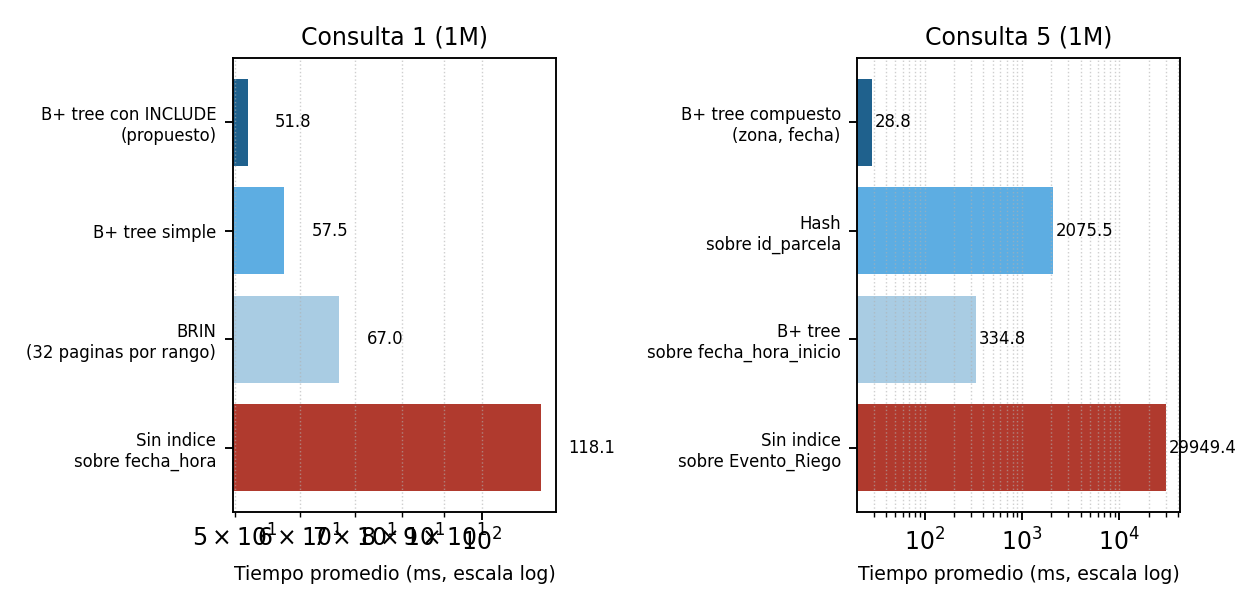
\includegraphics[width=0.95\textwidth]{figuras/tipos_indice.png}
\caption{Tiempo promedio según el tipo de índice (1M, escala logarítmica).}
\end{figure}

El resultado más útil para este dominio es el del BRIN. Guarda solo el valor mínimo y máximo de la fecha por cada bloque de 32 páginas, por eso ocupa 24~KB frente a los casi 30~MB del B+ tree con \tb{INCLUDE}, y se construye cinco veces más rápido. Aun así logra el 77~\% de la mejora del B+ tree (67~ms frente a 52~ms, partiendo de 118~ms). Funciona porque las lecturas están guardadas en orden cronológico: cada bloque contiene un intervalo de tiempo estrecho y el índice descarta la mayoría de bloques sin leerlos. Si las lecturas llegaran desordenadas, el BRIN no serviría.

En la consulta 5, el hash sobre la parcela solo resuelve la primera igualdad: encuentra todos los riegos de la parcela y debe filtrar zona y fecha fila por fila, por eso tarda 72 veces más que el B+ tree compuesto. El B+ tree sobre la fecha recorre el rango de seis horas de toda la empresa y filtra la zona, lo que lo deja en un punto intermedio. Un índice solo es tan bueno como su coincidencia con el patrón de búsqueda: el orden y la combinación de columnas pesan más que el tipo de estructura.

\subsubsection{Costo de los índices en las operaciones de escritura}

\begin{table}[H]
\centering\small
\resizebox{\textwidth}{!}{\begin{tabular}{lrrrrrr}
\toprule
Operación & Filas & Sin (ms) & Desv. & Con (ms) & Desv. & Sobrecosto \\
\midrule
Insercion de 20 000 lecturas & 20\,000 & 167.63 & 3.853 & 238.34 & 9.828 & +42~\% \\
Actualizacion de humedad (sensores 1 a 60) & 17\,083 & 84.62 & 19.02 & 148.26 & 25.75 & +75~\% \\
Insercion de 5 000 eventos de riego & 5\,000 & 66.60 & 2.339 & 74.31 & 4.604 & +12~\% \\
\bottomrule
\end{tabular}}
\caption{Costo de escritura con y sin los índices de optimización (1M, 5 iteraciones).}\label{tab:escritura}
\end{table}


\begin{figure}[H]
\centering
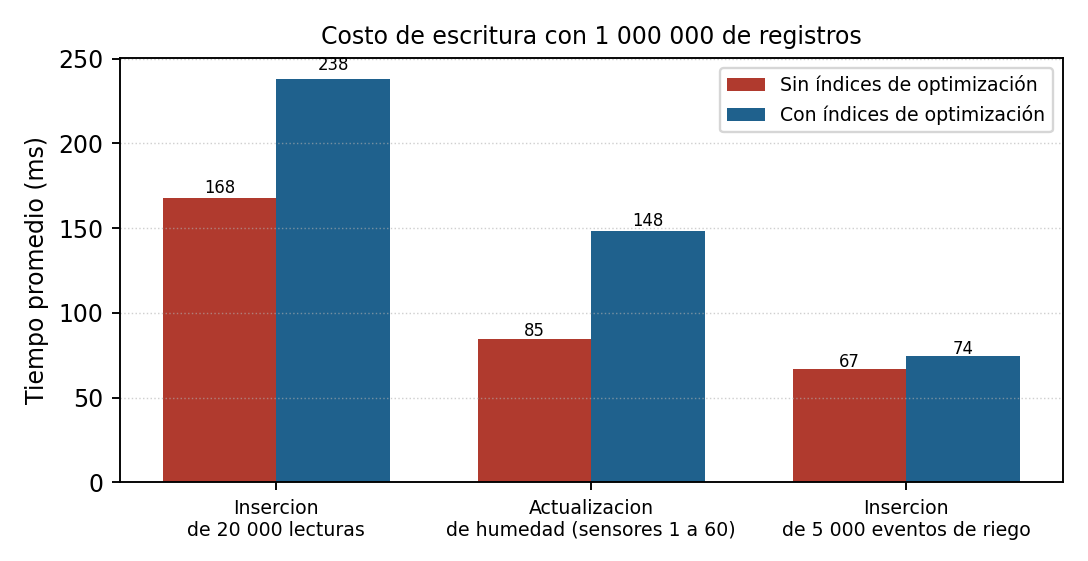
\includegraphics[width=0.78\textwidth]{figuras/escritura.png}
\caption{Tiempo de las operaciones de escritura con y sin índices de optimización (1M).}
\end{figure}

Los índices tienen un precio. Insertar 20\,000 lecturas cuesta 42~\% más con los índices de optimización, porque cada fila debe insertarse en tres árboles en lugar de uno. La actualización de humedad es la más afectada (75~\%): la columna \tb{humedad\_pct} está incluida en dos índices, así que PostgreSQL no puede hacer una actualización HOT (en la misma página, sin tocar índices) y debe escribir una entrada nueva en cada índice. En \tb{Evento\_Riego}, con un solo índice adicional, el sobrecosto es de 12~\%. La Tabla~\ref{tab:tamidx} muestra el espacio que ocupa cada índice.

\begin{table}[H]
\centering\small
\begin{tabular}{lllrl}
\toprule
Tabla & Índice & Tipo & Tamaño (KB) & Origen \\
\midrule
Alerta & \texttt{uq\_alerta} & B+ tree & 1\,464 & UNIQUE \\
Alerta & \texttt{idx\_alerta\_humedad\_baja} & B+ tree & 1\,024 & Optimización \\
Alerta & \texttt{pk\_alerta} & B+ tree & 672 & Clave primaria \\
Campania & \texttt{pk\_campania} & B+ tree & 56 & Clave primaria \\
Campania & \texttt{uq\_campania} & B+ tree & 56 & UNIQUE \\
Campania & \texttt{idx\_campania\_vigente} & B+ tree & 32 & Optimización \\
Campania & \texttt{idx\_campania\_cultivo} & B+ tree & 32 & Optimización \\
Cosecha & \texttt{idx\_cosecha\_campania} & Hash & 1\,040 & Optimización \\
Cosecha & \texttt{idx\_cosecha\_categoria} & B+ tree & 1\,008 & Optimización \\
Cosecha & \texttt{pk\_cosecha} & B+ tree & 568 & Clave primaria \\
Dispositivo & \texttt{uq\_dispositivo\_ser} & B+ tree & 104 & UNIQUE \\
Dispositivo & \texttt{pk\_dispositivo} & B+ tree & 80 & Clave primaria \\
Dispositivo & \texttt{idx\_dispositivo\_zona} & B+ tree & 80 & Optimización \\
Evento\_Riego & \texttt{idx\_evento\_parcela\_fecha} & B+ tree & 3\,720 & Optimización \\
Evento\_Riego & \texttt{uq\_evento} & B+ tree & 3\,720 & UNIQUE \\
Evento\_Riego & \texttt{pk\_evento} & B+ tree & 2\,656 & Clave primaria \\
Lectura\_Suelo & \texttt{idx\_lectura\_fecha} & B+ tree & 30\,336 & Optimización \\
Lectura\_Suelo & \texttt{idx\_lectura\_disp\_humedad} & B+ tree & 23\,608 & Optimización \\
Lectura\_Suelo & \texttt{pk\_lectura} & B+ tree & 23\,608 & Clave primaria \\
\bottomrule
\end{tabular}
\caption{Índices de las tablas involucradas (1M).}\label{tab:tamidx}
\end{table}


\subsection{Resultados}

\subsubsection{Consulta 1}

\begin{figure}[H]
\centering
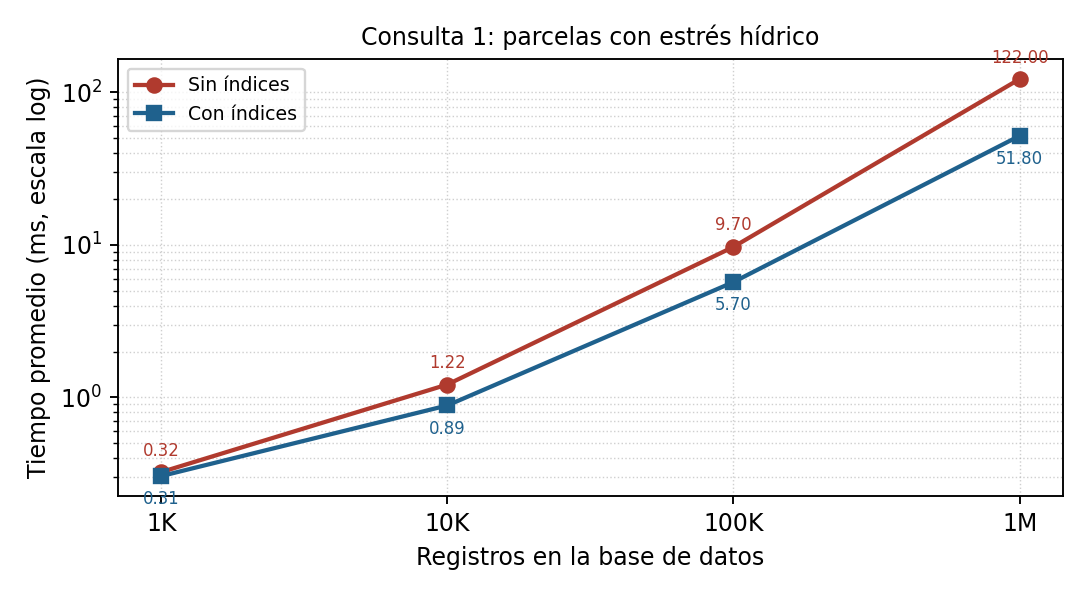
\includegraphics[width=0.78\textwidth]{figuras/consulta1.png}
\caption{Consulta 1: tiempo promedio por escenario.}
\end{figure}

\begin{table}[H]
\centering\small
\begin{tabular}{lrrrr}
\toprule
Escenario & Sin índices (ms) & Con índices (ms) & Relación sin/con & Filas devueltas \\
\midrule
1K & 0.325 & 0.306 & 1.06 & 2 \\
10K & 1.216 & 0.887 & 1.37 & 10 \\
100K & 9.701 & 5.705 & 1.70 & 39 \\
1M & 122.00 & 51.80 & 2.36 & 116 \\
\bottomrule
\end{tabular}
\caption{Consulta 1: promedios y relación de mejora.}
\end{table}


El índice mejora la consulta a partir de 10\,000 registros y con un millón la acelera 2.4 veces. Sin índice, PostgreSQL recorre las 765\,861 lecturas con un \emph{Parallel Seq Scan} y descarta nueve de cada diez. Con el índice, el \emph{Index Only Scan} sobre \tb{idx\_lectura\_fecha} lee solo las 77\,020 lecturas del último mes. Los índices sobre campañas y dispositivos no se usan: esas tablas tienen pocos miles de filas y el planificador las recorre completas porque le resulta más barato.

\textbf{Plan de ejecución sin índices (1M)}
\begin{lstlisting}[style=plano]
Sort (actual time=118.423..118.500 rows=116 loops=1)
Sort Key: (round(avg(l.humedad_pct), 2))
Sort Method: quicksort  Memory: 33kB
->  Finalize HashAggregate (actual time=118.132..118.447 rows=116 loops=1)
  Group Key: f.nombre, p.codigo_parcela, cu.nombre_comun
  Filter: (avg(l.humedad_pct) < min(cu.humedad_optima_min))
  Batches: 1  Memory Usage: 913kB
  Rows Removed by Filter: 418
  ->  Gather (actual time=112.133..117.039 rows=1602 loops=1)
    Workers Planned: 2
    Workers Launched: 2
    ->  Partial HashAggregate (actual time=104.522..104.728 rows=534 loops=3)
      Group Key: f.nombre, p.codigo_parcela, cu.nombre_comun
      Batches: 1  Memory Usage: 657kB
      Worker 0:  Batches: 1  Memory Usage: 657kB
      Worker 1:  Batches: 1  Memory Usage: 657kB
      ->  Hash Join (actual time=55.064..73.298 rows=23118 loops=3)
        Hash Cond: (l.id_dispositivo = s.id_dispositivo)
        ->  Parallel Seq Scan on lectura_suelo l (actual time=43.527..55.417 rows=25673 loops=3)
          Filter: ((humedad_pct IS NOT NULL) AND (fecha_hora >= '2026-08-16 00:00:00'::timestamp without time zone) AND (fecha_hora < '2026-09-16 00:00:00'::timestamp without time zone))
          Rows Removed by Filter: 229614
        ->  Hash (actual time=11.493..11.502 rows=1971 loops=3)
          Buckets: 2048  Batches: 1  Memory Usage: 159kB
          ->  Hash Join (actual time=1.614..8.381 rows=1971 loops=3)
            Hash Cond: ((d.id_parcela = z.id_parcela) AND (d.num_zona = z.num_zona))
            ->  Hash Join (actual time=1.110..7.544 rows=1971 loops=3)
              Hash Cond: (d.id_parcela = p.id_parcela)
              ->  Hash Join (actual time=0.417..3.774 rows=2200 loops=3)
                Hash Cond: (d.id_dispositivo = s.id_dispositivo)
                ->  Seq Scan on dispositivo d (actual time=0.008..0.193 rows=2800 loops=3)
                ->  Hash (actual time=0.386..0.387 rows=2200 loops=3)
                  Buckets: 4096  Batches: 1  Memory Usage: 110kB
                  ->  Seq Scan on sensor s (actual time=0.005..0.174 rows=2200 loops=3)
              ->  Hash (actual time=0.682..0.687 rows=539 loops=3)
                Buckets: 1024  Batches: 1  Memory Usage: 49kB
                ->  Hash Join (actual time=0.204..0.570 rows=539 loops=3)
                  Hash Cond: (ca.id_cultivo = cu.id_cultivo)
                  ->  Hash Join (actual time=0.180..0.471 rows=539 loops=3)
                    Hash Cond: (p.id_fundo = f.id_fundo)
                    ->  Hash Join (actual time=0.155..0.372 rows=539 loops=3)
                      Hash Cond: (ca.id_parcela = p.id_parcela)
                      ->  Seq Scan on campania ca (actual time=0.004..0.139 rows=539 loops=3)
                        Filter: ((estado)::text = 'En curso'::text)
                        Rows Removed by Filter: 961
                      ->  Hash (actual time=0.135..0.135 rows=600 loops=3)
                        Buckets: 1024  Batches: 1  Memory Usage: 37kB
                        ->  Seq Scan on parcela p (actual time=0.006..0.057 rows=600 loops=3)
                    ->  Hash (actual time=0.016..0.017 rows=12 loops=3)
                      Buckets: 1024  Batches: 1  Memory Usage: 9kB
                      ->  Seq Scan on fundo f (actual time=0.010..0.011 rows=12 loops=3)
                  ->  Hash (actual time=0.013..0.014 rows=12 loops=3)
                    Buckets: 1024  Batches: 1  Memory Usage: 9kB
                    ->  Seq Scan on cultivo cu (actual time=0.006..0.007 rows=12 loops=3)
            ->  Hash (actual time=0.475..0.475 rows=2400 loops=3)
              Buckets: 4096  Batches: 1  Memory Usage: 122kB
              ->  Seq Scan on zona_manejo z (actual time=0.013..0.217 rows=2400 loops=3)
Planning Time: 3.552 ms
Execution Time: 118.710 ms
\end{lstlisting}

\textbf{Plan de ejecución con índices (1M)}
\begin{lstlisting}[style=plano]
Sort (actual time=49.632..49.647 rows=116 loops=1)
Sort Key: (round(avg(l.humedad_pct), 2))
Sort Method: quicksort  Memory: 33kB
->  HashAggregate (actual time=49.378..49.594 rows=116 loops=1)
  Group Key: f.nombre, p.codigo_parcela, cu.nombre_comun
  Filter: (avg(l.humedad_pct) < min(cu.humedad_optima_min))
  Batches: 1  Memory Usage: 657kB
  Rows Removed by Filter: 418
  ->  Hash Join (actual time=3.176..27.939 rows=69353 loops=1)
    Hash Cond: (l.id_dispositivo = s.id_dispositivo)
    ->  Index Only Scan using idx_lectura_fecha on lectura_suelo l (actual time=0.012..10.757 rows=77020 loops=1)
      Index Cond: ((fecha_hora >= '2026-08-16 00:00:00'::timestamp without time zone) AND (fecha_hora < '2026-09-16 00:00:00'::timestamp without time zone))
      Filter: (humedad_pct IS NOT NULL)
      Rows Removed by Filter: 14931
      Heap Fetches: 0
    ->  Hash (actual time=3.160..3.167 rows=1971 loops=1)
      Buckets: 2048  Batches: 1  Memory Usage: 159kB
      ->  Hash Join (actual time=1.450..2.776 rows=1971 loops=1)
        Hash Cond: ((d.id_parcela = z.id_parcela) AND (d.num_zona = z.num_zona))
        ->  Hash Join (actual time=0.970..1.982 rows=1971 loops=1)
          Hash Cond: (d.id_parcela = p.id_parcela)
          ->  Hash Join (actual time=0.356..0.995 rows=2200 loops=1)
            Hash Cond: (d.id_dispositivo = s.id_dispositivo)
            ->  Seq Scan on dispositivo d (actual time=0.002..0.182 rows=2800 loops=1)
            ->  Hash (actual time=0.349..0.350 rows=2200 loops=1)
              Buckets: 4096  Batches: 1  Memory Usage: 110kB
              ->  Seq Scan on sensor s (actual time=0.003..0.165 rows=2200 loops=1)
          ->  Hash (actual time=0.610..0.614 rows=539 loops=1)
            Buckets: 1024  Batches: 1  Memory Usage: 49kB
            ->  Hash Join (actual time=0.146..0.511 rows=539 loops=1)
              Hash Cond: (ca.id_cultivo = cu.id_cultivo)
              ->  Hash Join (actual time=0.136..0.427 rows=539 loops=1)
                Hash Cond: (p.id_fundo = f.id_fundo)
                ->  Hash Join (actual time=0.128..0.347 rows=539 loops=1)
                  Hash Cond: (ca.id_parcela = p.id_parcela)
                  ->  Seq Scan on campania ca (actual time=0.003..0.140 rows=539 loops=1)
                    Filter: ((estado)::text = 'En curso'::text)
                    Rows Removed by Filter: 961
                  ->  Hash (actual time=0.121..0.121 rows=600 loops=1)
                    Buckets: 1024  Batches: 1  Memory Usage: 37kB
                    ->  Seq Scan on parcela p (actual time=0.003..0.059 rows=600 loops=1)
                ->  Hash (actual time=0.005..0.006 rows=12 loops=1)
                  Buckets: 1024  Batches: 1  Memory Usage: 9kB
                  ->  Seq Scan on fundo f (actual time=0.002..0.003 rows=12 loops=1)
              ->  Hash (actual time=0.007..0.007 rows=12 loops=1)
                Buckets: 1024  Batches: 1  Memory Usage: 9kB
                ->  Seq Scan on cultivo cu (actual time=0.003..0.004 rows=12 loops=1)
        ->  Hash (actual time=0.475..0.475 rows=2400 loops=1)
          Buckets: 4096  Batches: 1  Memory Usage: 122kB
          ->  Seq Scan on zona_manejo z (actual time=0.006..0.200 rows=2400 loops=1)
Planning Time: 3.962 ms
Execution Time: 49.742 ms
\end{lstlisting}


\subsubsection{Consulta 2}

\begin{figure}[H]
\centering
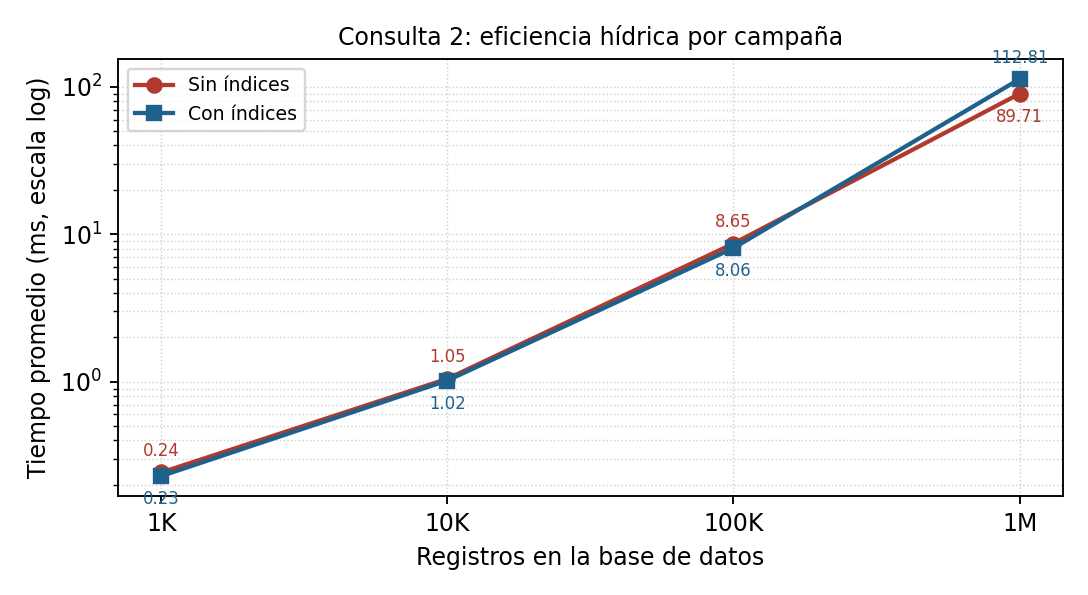
\includegraphics[width=0.78\textwidth]{figuras/consulta2.png}
\caption{Consulta 2: tiempo promedio por escenario.}
\end{figure}

\begin{table}[H]
\centering\small
\begin{tabular}{lrrrr}
\toprule
Escenario & Sin índices (ms) & Con índices (ms) & Relación sin/con & Filas devueltas \\
\midrule
1K & 0.243 & 0.229 & 1.06 & 0 \\
10K & 1.047 & 1.020 & 1.03 & 7 \\
100K & 8.651 & 8.061 & 1.07 & 58 \\
1M & 89.71 & 112.81 & 0.80 (más lenta) & 159 \\
\bottomrule
\end{tabular}
\caption{Consulta 2: promedios y relación de mejora.}
\end{table}


Es el caso en que el índice perjudica. Hasta 100\,000 registros la versión con índices es ligeramente más rápida, pero con un millón es 26~\% más lenta. Sin índices, el plan lee una sola vez los 120\,000 riegos y los une con las campañas mediante un \emph{Hash Join}. Con índices, el planificador cambia a un \emph{Nested Loop}: por cada una de las 1\,500 campañas desciende por \tb{idx\_evento\_parcela\_fecha} y agrega un nodo \emph{Memoize} para reutilizar búsquedas repetidas. Ese caché no acierta ni una vez (0 aciertos, 1\,500 fallos) porque cada campaña tiene un rango de fechas distinto. Mil quinientos descensos por el índice más el costo del caché inútil superan a un único recorrido secuencial. El planificador estimó mal y solo la medición lo revela.

\textbf{Plan de ejecución sin índices (1M)}
\begin{lstlisting}[style=plano]
Sort (actual time=85.733..85.816 rows=159 loops=1)
Sort Key: (round((r.litros_aplicados / pr.kilos), 2)) DESC
Sort Method: quicksort  Memory: 37kB
CTE riego
 ->  Finalize HashAggregate (actual time=76.102..76.432 rows=1095 loops=1)
   Group Key: ca_1.id_campania
   Batches: 1  Memory Usage: 577kB
   ->  Gather (actual time=73.451..75.096 rows=2165 loops=1)
     Workers Planned: 1
     Workers Launched: 1
     ->  Partial HashAggregate (actual time=69.902..70.184 rows=1082 loops=2)
       Group Key: ca_1.id_campania
       Batches: 1  Memory Usage: 577kB
       Worker 0:  Batches: 1  Memory Usage: 577kB
       ->  Hash Join (actual time=0.340..46.863 rows=52198 loops=2)
         Hash Cond: (er.id_parcela = ca_1.id_parcela)
         Join Filter: ((er.fecha_hora_inicio >= ca_1.fecha_siembra) AND (er.fecha_hora_inicio < ca_1.fecha_fin_estimada))
         Rows Removed by Join Filter: 98268
         ->  Parallel Seq Scan on evento_riego er (actual time=0.003..4.063 rows=60000 loops=2)
         ->  Hash (actual time=0.317..0.318 rows=1500 loops=2)
           Buckets: 2048  Batches: 1  Memory Usage: 87kB
           ->  Seq Scan on campania ca_1 (actual time=0.008..0.135 rows=1500 loops=2)
InitPlan 2 (returns $2)
 ->  Aggregate (actual time=0.595..0.596 rows=1 loops=1)
   ->  CTE Scan on riego (actual time=0.001..0.443 rows=1095 loops=1)
->  Hash Join (actual time=85.120..85.673 rows=159 loops=1)
  Hash Cond: (r.id_campania = pr.id_campania)
  ->  Hash Join (actual time=77.144..77.578 rows=323 loops=1)
    Hash Cond: (ca.id_cultivo = cu.id_cultivo)
    ->  Hash Join (actual time=77.132..77.519 rows=323 loops=1)
      Hash Cond: (p.id_fundo = f.id_fundo)
      ->  Hash Join (actual time=77.123..77.462 rows=323 loops=1)
        Hash Cond: (ca.id_parcela = p.id_parcela)
        ->  Hash Join (actual time=77.008..77.280 rows=323 loops=1)
          Hash Cond: (r.id_campania = ca.id_campania)
          ->  CTE Scan on riego r (actual time=76.706..76.907 rows=323 loops=1)
            Filter: (litros_aplicados > $2)
            Rows Removed by Filter: 772
          ->  Hash (actual time=0.293..0.293 rows=1500 loops=1)
            Buckets: 2048  Batches: 1  Memory Usage: 81kB
            ->  Seq Scan on campania ca (actual time=0.009..0.141 rows=1500 loops=1)
        ->  Hash (actual time=0.111..0.112 rows=600 loops=1)
          Buckets: 1024  Batches: 1  Memory Usage: 32kB
          ->  Seq Scan on parcela p (actual time=0.002..0.054 rows=600 loops=1)
      ->  Hash (actual time=0.006..0.006 rows=12 loops=1)
        Buckets: 1024  Batches: 1  Memory Usage: 9kB
        ->  Seq Scan on fundo f (actual time=0.003..0.004 rows=12 loops=1)
    ->  Hash (actual time=0.009..0.010 rows=12 loops=1)
      Buckets: 1024  Batches: 1  Memory Usage: 9kB
      ->  Seq Scan on cultivo cu (actual time=0.004..0.006 rows=12 loops=1)
  ->  Hash (actual time=7.957..7.959 rows=902 loops=1)
    Buckets: 1024  Batches: 1  Memory Usage: 50kB
    ->  Subquery Scan on pr (actual time=7.563..7.842 rows=902 loops=1)
      ->  HashAggregate (actual time=7.561..7.763 rows=902 loops=1)
        Group Key: cosecha.id_campania
        Batches: 1  Memory Usage: 553kB
        ->  Seq Scan on cosecha (actual time=0.004..2.737 rows=25000 loops=1)
Planning Time: 0.800 ms
Execution Time: 85.911 ms
\end{lstlisting}

\textbf{Plan de ejecución con índices (1M)}
\begin{lstlisting}[style=plano]
Sort (actual time=105.264..105.280 rows=159 loops=1)
Sort Key: (round((r.litros_aplicados / pr.kilos), 2)) DESC
Sort Method: quicksort  Memory: 37kB
CTE riego
 ->  GroupAggregate (actual time=0.082..96.307 rows=1095 loops=1)
   Group Key: ca_1.id_campania
   ->  Nested Loop (actual time=0.016..79.549 rows=104397 loops=1)
     ->  Index Scan using pk_campania on campania ca_1 (actual time=0.006..0.364 rows=1500 loops=1)
     ->  Memoize (actual time=0.004..0.046 rows=70 loops=1500)
       Cache Key: ca_1.fecha_siembra, ca_1.fecha_fin_estimada, ca_1.id_parcela
       Cache Mode: binary
       Hits: 0  Misses: 1500  Evictions: 0  Overflows: 0  Memory Usage: 5821kB
       ->  Index Scan using idx_evento_parcela_fecha on evento_riego er (actual time=0.003..0.026 rows=70 loops=1500)
         Index Cond: ((id_parcela = ca_1.id_parcela) AND (fecha_hora_inicio >= ca_1.fecha_siembra) AND (fecha_hora_inicio < ca_1.fecha_fin_estimada))
InitPlan 2 (returns $4)
 ->  Aggregate (actual time=96.801..96.802 rows=1 loops=1)
   ->  CTE Scan on riego (actual time=0.000..96.537 rows=1095 loops=1)
->  Hash Join (actual time=104.606..105.201 rows=159 loops=1)
  Hash Cond: (r.id_campania = pr.id_campania)
  ->  Hash Join (actual time=97.308..97.770 rows=323 loops=1)
    Hash Cond: (ca.id_cultivo = cu.id_cultivo)
    ->  Hash Join (actual time=97.296..97.706 rows=323 loops=1)
      Hash Cond: (p.id_fundo = f.id_fundo)
      ->  Hash Join (actual time=97.287..97.648 rows=323 loops=1)
        Hash Cond: (ca.id_parcela = p.id_parcela)
        ->  Hash Join (actual time=97.172..97.455 rows=323 loops=1)
          Hash Cond: (r.id_campania = ca.id_campania)
          ->  CTE Scan on riego r (actual time=96.888..97.095 rows=323 loops=1)
            Filter: (litros_aplicados > $4)
            Rows Removed by Filter: 772
          ->  Hash (actual time=0.275..0.276 rows=1500 loops=1)
            Buckets: 2048  Batches: 1  Memory Usage: 81kB
            ->  Seq Scan on campania ca (actual time=0.009..0.133 rows=1500 loops=1)
        ->  Hash (actual time=0.111..0.112 rows=600 loops=1)
          Buckets: 1024  Batches: 1  Memory Usage: 32kB
          ->  Seq Scan on parcela p (actual time=0.002..0.053 rows=600 loops=1)
      ->  Hash (actual time=0.005..0.006 rows=12 loops=1)
        Buckets: 1024  Batches: 1  Memory Usage: 9kB
        ->  Seq Scan on fundo f (actual time=0.001..0.003 rows=12 loops=1)
    ->  Hash (actual time=0.009..0.009 rows=12 loops=1)
      Buckets: 1024  Batches: 1  Memory Usage: 9kB
      ->  Seq Scan on cultivo cu (actual time=0.003..0.005 rows=12 loops=1)
  ->  Hash (actual time=7.290..7.291 rows=902 loops=1)
    Buckets: 1024  Batches: 1  Memory Usage: 50kB
    ->  Subquery Scan on pr (actual time=6.854..7.176 rows=902 loops=1)
      ->  HashAggregate (actual time=6.852..7.076 rows=902 loops=1)
        Group Key: cosecha.id_campania
        Batches: 1  Memory Usage: 553kB
        ->  Seq Scan on cosecha (actual time=0.003..1.765 rows=25000 loops=1)
Planning Time: 0.879 ms
Execution Time: 105.374 ms
\end{lstlisting}


\subsubsection{Consulta 3}

\begin{figure}[H]
\centering
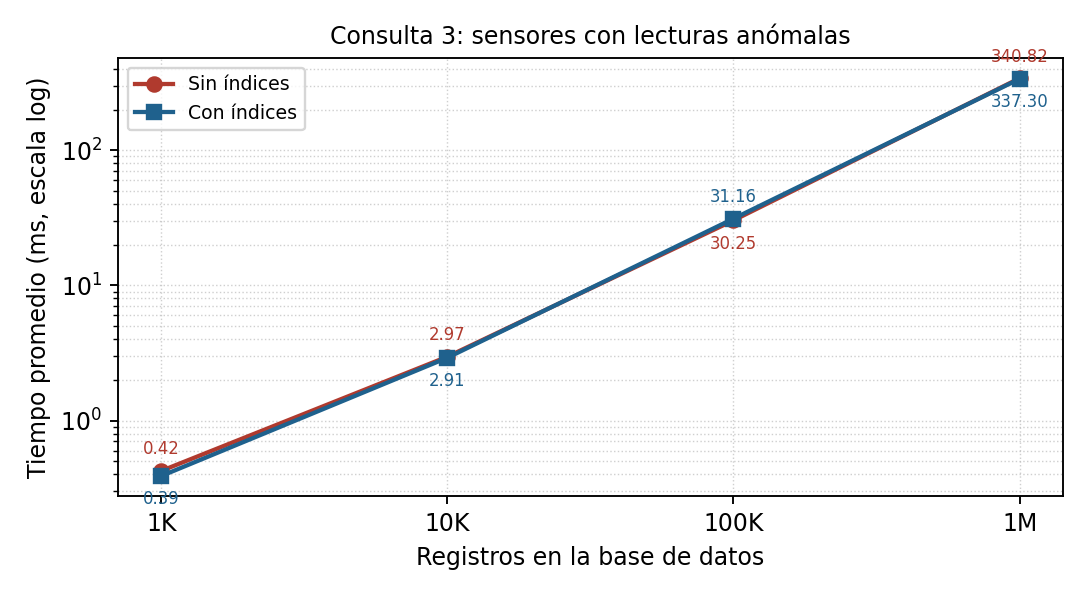
\includegraphics[width=0.78\textwidth]{figuras/consulta3.png}
\caption{Consulta 3: tiempo promedio por escenario.}
\end{figure}

\begin{table}[H]
\centering\small
\begin{tabular}{lrrrr}
\toprule
Escenario & Sin índices (ms) & Con índices (ms) & Relación sin/con & Filas devueltas \\
\midrule
1K & 0.424 & 0.389 & 1.09 & 8 \\
10K & 2.967 & 2.914 & 1.02 & 25 \\
100K & 30.25 & 31.16 & 0.97 (más lenta) & 110 \\
1M & 340.82 & 337.30 & 1.01 & 359 \\
\bottomrule
\end{tabular}
\caption{Consulta 3: promedios y relación de mejora.}
\end{table}


Los tiempos son prácticamente iguales en las dos condiciones y el plan es el mismo: un recorrido secuencial paralelo de toda la tabla de lecturas. La consulta necesita el 84~\% de las filas, y para ese volumen leer la tabla en orden físico es más barato que recorrer un índice. El índice \tb{idx\_lectura\_disp\_humedad} ocupa 24~MB y nunca se usa.

\textbf{Plan de ejecución sin índices (1M)}
\begin{lstlisting}[style=plano]
Sort (actual time=324.220..324.318 rows=359 loops=1)
Sort Key: (round(((100.0 * (m.anomalas)::numeric) / (m.total)::numeric), 2)) DESC, m.total DESC
Sort Method: quicksort  Memory: 53kB
CTE medidas
 ->  Finalize HashAggregate (actual time=319.637..319.899 rows=1693 loops=1)
   Group Key: l.id_dispositivo
   Batches: 1  Memory Usage: 369kB
   ->  Gather (actual time=315.349..318.795 rows=5079 loops=1)
     Workers Planned: 2
     Workers Launched: 2
     ->  Partial HashAggregate (actual time=309.122..309.317 rows=1693 loops=3)
       Group Key: l.id_dispositivo
       Batches: 1  Memory Usage: 369kB
       Worker 0:  Batches: 1  Memory Usage: 369kB
       Worker 1:  Batches: 1  Memory Usage: 369kB
       ->  Hash Join (actual time=3.992..161.661 rows=192566 loops=3)
         Hash Cond: (l.id_dispositivo = d_1.id_dispositivo)
         ->  Parallel Seq Scan on lectura_suelo l (actual time=0.015..70.872 rows=213710 loops=3)
           Filter: (humedad_pct IS NOT NULL)
           Rows Removed by Filter: 41577
         ->  Hash (actual time=3.951..3.955 rows=2509 loops=3)
           Buckets: 4096  Batches: 1  Memory Usage: 145kB
           ->  Hash Join (actual time=0.302..3.679 rows=2509 loops=3)
             Hash Cond: (d_1.id_parcela = ca.id_parcela)
             ->  Seq Scan on dispositivo d_1 (actual time=0.005..0.180 rows=2800 loops=3)
             ->  Hash (actual time=0.287..0.290 rows=539 loops=3)
               Buckets: 1024  Batches: 1  Memory Usage: 33kB
               ->  Hash Join (actual time=0.032..0.223 rows=539 loops=3)
                 Hash Cond: (ca.id_cultivo = cu.id_cultivo)
                 ->  Seq Scan on campania ca (actual time=0.008..0.121 rows=539 loops=3)
                   Filter: ((estado)::text = 'En curso'::text)
                   Rows Removed by Filter: 961
                 ->  Hash (actual time=0.014..0.015 rows=12 loops=3)
                   Buckets: 1024  Batches: 1  Memory Usage: 9kB
                   ->  Seq Scan on cultivo cu (actual time=0.007..0.009 rows=12 loops=3)
InitPlan 2 (returns $2)
 ->  Aggregate (actual time=0.652..0.652 rows=1 loops=1)
   ->  CTE Scan on medidas (actual time=0.001..0.523 rows=1693 loops=1)
->  Hash Join (actual time=323.425..324.057 rows=359 loops=1)
  Hash Cond: (d.id_parcela = p.id_parcela)
  ->  Hash Join (actual time=323.312..323.765 rows=359 loops=1)
    Hash Cond: (d.id_dispositivo = s.id_dispositivo)
    ->  Seq Scan on dispositivo d (actual time=0.001..0.180 rows=2800 loops=1)
    ->  Hash (actual time=323.304..323.305 rows=359 loops=1)
      Buckets: 1024  Batches: 1  Memory Usage: 33kB
      ->  Hash Join (actual time=320.790..323.230 rows=359 loops=1)
        Hash Cond: (m.id_dispositivo = s.id_dispositivo)
        ->  CTE Scan on medidas m (actual time=320.300..322.663 rows=359 loops=1)
          Filter: ((total >= 5) AND (((1.0 * (anomalas)::numeric) / (total)::numeric) > $2))
          Rows Removed by Filter: 1334
        ->  Hash (actual time=0.477..0.477 rows=2200 loops=1)
          Buckets: 4096  Batches: 1  Memory Usage: 135kB
          ->  Seq Scan on sensor s (actual time=0.009..0.181 rows=2200 loops=1)
  ->  Hash (actual time=0.108..0.108 rows=600 loops=1)
    Buckets: 1024  Batches: 1  Memory Usage: 34kB
    ->  Seq Scan on parcela p (actual time=0.004..0.054 rows=600 loops=1)
Planning Time: 0.649 ms
Execution Time: 324.423 ms
\end{lstlisting}

\textbf{Plan de ejecución con índices (1M)}
\begin{lstlisting}[style=plano]
Sort (actual time=322.806..322.894 rows=359 loops=1)
Sort Key: (round(((100.0 * (m.anomalas)::numeric) / (m.total)::numeric), 2)) DESC, m.total DESC
Sort Method: quicksort  Memory: 53kB
CTE medidas
 ->  Finalize HashAggregate (actual time=318.307..318.572 rows=1693 loops=1)
   Group Key: l.id_dispositivo
   Batches: 1  Memory Usage: 369kB
   ->  Gather (actual time=313.694..317.475 rows=5079 loops=1)
     Workers Planned: 2
     Workers Launched: 2
     ->  Partial HashAggregate (actual time=308.832..309.029 rows=1693 loops=3)
       Group Key: l.id_dispositivo
       Batches: 1  Memory Usage: 369kB
       Worker 0:  Batches: 1  Memory Usage: 369kB
       Worker 1:  Batches: 1  Memory Usage: 369kB
       ->  Hash Join (actual time=3.991..184.920 rows=192566 loops=3)
         Hash Cond: (l.id_dispositivo = d_1.id_dispositivo)
         ->  Parallel Seq Scan on lectura_suelo l (actual time=0.014..63.854 rows=213710 loops=3)
           Filter: (humedad_pct IS NOT NULL)
           Rows Removed by Filter: 41577
         ->  Hash (actual time=3.954..3.959 rows=2509 loops=3)
           Buckets: 4096  Batches: 1  Memory Usage: 145kB
           ->  Hash Join (actual time=0.297..0.993 rows=2509 loops=3)
             Hash Cond: (d_1.id_parcela = ca.id_parcela)
             ->  Seq Scan on dispositivo d_1 (actual time=0.003..0.186 rows=2800 loops=3)
             ->  Hash (actual time=0.285..0.287 rows=539 loops=3)
               Buckets: 1024  Batches: 1  Memory Usage: 33kB
               ->  Hash Join (actual time=0.030..0.229 rows=539 loops=3)
                 Hash Cond: (ca.id_cultivo = cu.id_cultivo)
                 ->  Seq Scan on campania ca (actual time=0.007..0.127 rows=539 loops=3)
                   Filter: ((estado)::text = 'En curso'::text)
                   Rows Removed by Filter: 961
                 ->  Hash (actual time=0.014..0.015 rows=12 loops=3)
                   Buckets: 1024  Batches: 1  Memory Usage: 9kB
                   ->  Seq Scan on cultivo cu (actual time=0.007..0.009 rows=12 loops=3)
InitPlan 2 (returns $2)
 ->  Aggregate (actual time=0.632..0.633 rows=1 loops=1)
   ->  CTE Scan on medidas (actual time=0.001..0.517 rows=1693 loops=1)
->  Hash Join (actual time=320.296..322.637 rows=359 loops=1)
  Hash Cond: (d.id_parcela = p.id_parcela)
  ->  Hash Join (actual time=320.184..322.336 rows=359 loops=1)
    Hash Cond: (d.id_dispositivo = s.id_dispositivo)
    ->  Seq Scan on dispositivo d (actual time=0.001..1.874 rows=2800 loops=1)
    ->  Hash (actual time=320.177..320.178 rows=359 loops=1)
      Buckets: 1024  Batches: 1  Memory Usage: 33kB
      ->  Hash Join (actual time=319.443..320.108 rows=359 loops=1)
        Hash Cond: (m.id_dispositivo = s.id_dispositivo)
        ->  CTE Scan on medidas m (actual time=318.952..319.562 rows=359 loops=1)
          Filter: ((total >= 5) AND (((1.0 * (anomalas)::numeric) / (total)::numeric) > $2))
          Rows Removed by Filter: 1334
        ->  Hash (actual time=0.479..0.480 rows=2200 loops=1)
          Buckets: 4096  Batches: 1  Memory Usage: 135kB
          ->  Seq Scan on sensor s (actual time=0.008..0.180 rows=2200 loops=1)
  ->  Hash (actual time=0.107..0.107 rows=600 loops=1)
    Buckets: 1024  Batches: 1  Memory Usage: 34kB
    ->  Seq Scan on parcela p (actual time=0.004..0.054 rows=600 loops=1)
Planning Time: 0.810 ms
Execution Time: 323.000 ms
\end{lstlisting}


\subsubsection{Consulta 4}

\begin{figure}[H]
\centering
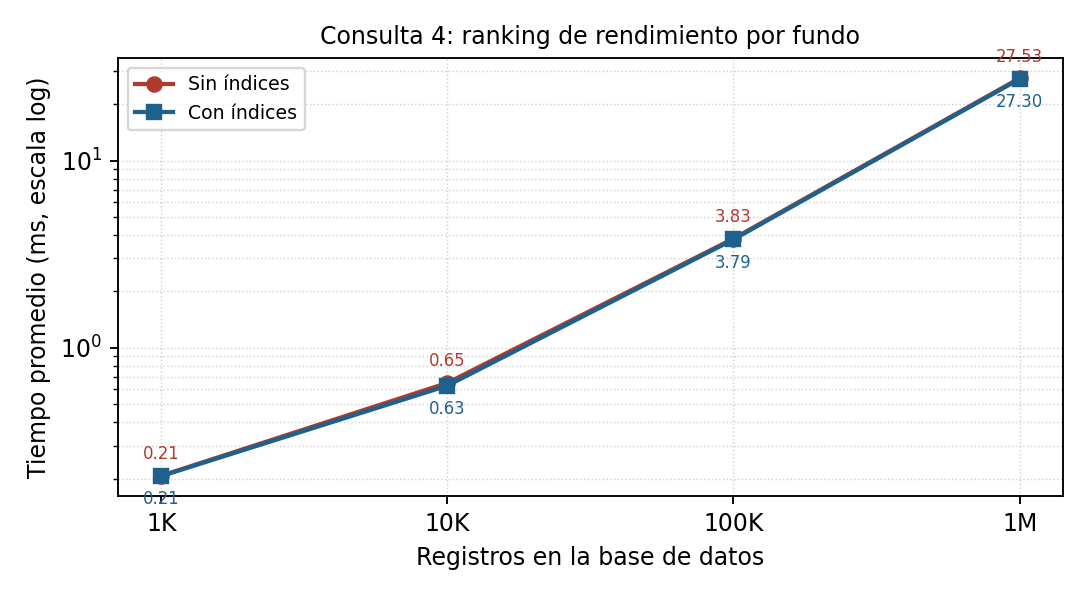
\includegraphics[width=0.78\textwidth]{figuras/consulta4.png}
\caption{Consulta 4: tiempo promedio por escenario.}
\end{figure}

\begin{table}[H]
\centering\small
\begin{tabular}{lrrrr}
\toprule
Escenario & Sin índices (ms) & Con índices (ms) & Relación sin/con & Filas devueltas \\
\midrule
1K & 0.207 & 0.206 & 1.00 & 10 \\
10K & 0.649 & 0.627 & 1.03 & 43 \\
100K & 3.827 & 3.791 & 1.01 & 195 \\
1M & 27.53 & 27.30 & 1.01 & 902 \\
\bottomrule
\end{tabular}
\caption{Consulta 4: promedios y relación de mejora.}
\end{table}


Tampoco hay diferencia. El filtro por categoría conserva el 82~\% de las cosechas (primera y segunda), así que el planificador vuelve a preferir el recorrido secuencial, y la tabla de cosechas es pequeña (25\,000 filas). La mayor parte del tiempo se va en las funciones de ventana y en el ordenamiento, que ningún índice acelera en este caso.

\textbf{Plan de ejecución sin índices (1M)}
\begin{lstlisting}[style=plano]
Sort (actual time=26.184..26.270 rows=902 loops=1)
Sort Key: rendimiento.fundo, (rank() OVER (?))
Sort Method: quicksort  Memory: 111kB
->  WindowAgg (actual time=24.438..25.414 rows=902 loops=1)
  ->  WindowAgg (actual time=24.359..24.814 rows=902 loops=1)
    ->  Sort (actual time=24.354..24.402 rows=902 loops=1)
      Sort Key: rendimiento.id_fundo, ((rendimiento.kilos / rendimiento.area_ha)) DESC
      Sort Method: quicksort  Memory: 104kB
      ->  Subquery Scan on rendimiento (actual time=22.940..23.434 rows=902 loops=1)
        ->  HashAggregate (actual time=22.937..23.230 rows=902 loops=1)
          Group Key: f.id_fundo, cu.nombre_comun, ca.id_campania, p.area_ha
          Batches: 1  Memory Usage: 1297kB
          ->  Hash Join (actual time=0.435..16.063 rows=20452 loops=1)
            Hash Cond: (ca.id_cultivo = cu.id_cultivo)
            ->  Hash Join (actual time=0.422..13.190 rows=20452 loops=1)
              Hash Cond: (p.id_fundo = f.id_fundo)
              ->  Hash Join (actual time=0.414..10.296 rows=20452 loops=1)
                Hash Cond: (ca.id_parcela = p.id_parcela)
                ->  Hash Join (actual time=0.296..7.078 rows=20452 loops=1)
                  Hash Cond: (co.id_campania = ca.id_campania)
                  ->  Seq Scan on cosecha co (actual time=0.003..3.583 rows=20452 loops=1)
                    Filter: ((categoria)::text = ANY ('{Primera,Segunda}'::text[]))
                    Rows Removed by Filter: 4548
                  ->  Hash (actual time=0.290..0.291 rows=1500 loops=1)
                    Buckets: 2048  Batches: 1  Memory Usage: 81kB
                    ->  Seq Scan on campania ca (actual time=0.002..0.124 rows=1500 loops=1)
                ->  Hash (actual time=0.115..0.115 rows=600 loops=1)
                  Buckets: 1024  Batches: 1  Memory Usage: 37kB
                  ->  Seq Scan on parcela p (actual time=0.002..0.054 rows=600 loops=1)
              ->  Hash (actual time=0.006..0.006 rows=12 loops=1)
                Buckets: 1024  Batches: 1  Memory Usage: 9kB
                ->  Seq Scan on fundo f (actual time=0.002..0.004 rows=12 loops=1)
            ->  Hash (actual time=0.010..0.011 rows=12 loops=1)
              Buckets: 1024  Batches: 1  Memory Usage: 9kB
              ->  Seq Scan on cultivo cu (actual time=0.004..0.006 rows=12 loops=1)
Planning Time: 0.471 ms
Execution Time: 26.434 ms
\end{lstlisting}

\textbf{Plan de ejecución con índices (1M)}
\begin{lstlisting}[style=plano]
Sort (actual time=26.507..26.557 rows=902 loops=1)
Sort Key: rendimiento.fundo, (rank() OVER (?))
Sort Method: quicksort  Memory: 111kB
->  WindowAgg (actual time=24.669..25.706 rows=902 loops=1)
  ->  WindowAgg (actual time=24.588..25.092 rows=902 loops=1)
    ->  Sort (actual time=24.581..24.632 rows=902 loops=1)
      Sort Key: rendimiento.id_fundo, ((rendimiento.kilos / rendimiento.area_ha)) DESC
      Sort Method: quicksort  Memory: 104kB
      ->  Subquery Scan on rendimiento (actual time=22.929..23.485 rows=902 loops=1)
        ->  HashAggregate (actual time=22.926..23.267 rows=902 loops=1)
          Group Key: f.id_fundo, cu.nombre_comun, ca.id_campania, p.area_ha
          Batches: 1  Memory Usage: 1297kB
          ->  Hash Join (actual time=0.401..16.217 rows=20452 loops=1)
            Hash Cond: (ca.id_cultivo = cu.id_cultivo)
            ->  Hash Join (actual time=0.387..13.325 rows=20452 loops=1)
              Hash Cond: (p.id_fundo = f.id_fundo)
              ->  Hash Join (actual time=0.380..10.350 rows=20452 loops=1)
                Hash Cond: (ca.id_parcela = p.id_parcela)
                ->  Hash Join (actual time=0.260..6.996 rows=20452 loops=1)
                  Hash Cond: (co.id_campania = ca.id_campania)
                  ->  Seq Scan on cosecha co (actual time=0.003..3.539 rows=20452 loops=1)
                    Filter: ((categoria)::text = ANY ('{Primera,Segunda}'::text[]))
                    Rows Removed by Filter: 4548
                  ->  Hash (actual time=0.253..0.254 rows=1500 loops=1)
                    Buckets: 2048  Batches: 1  Memory Usage: 81kB
                    ->  Seq Scan on campania ca (actual time=0.002..0.121 rows=1500 loops=1)
                ->  Hash (actual time=0.117..0.118 rows=600 loops=1)
                  Buckets: 1024  Batches: 1  Memory Usage: 37kB
                  ->  Seq Scan on parcela p (actual time=0.002..0.055 rows=600 loops=1)
              ->  Hash (actual time=0.005..0.006 rows=12 loops=1)
                Buckets: 1024  Batches: 1  Memory Usage: 9kB
                ->  Seq Scan on fundo f (actual time=0.002..0.003 rows=12 loops=1)
            ->  Hash (actual time=0.011..0.011 rows=12 loops=1)
              Buckets: 1024  Batches: 1  Memory Usage: 9kB
              ->  Seq Scan on cultivo cu (actual time=0.004..0.006 rows=12 loops=1)
Planning Time: 0.584 ms
Execution Time: 26.721 ms
\end{lstlisting}


\subsubsection{Consulta 5}

\begin{figure}[H]
\centering
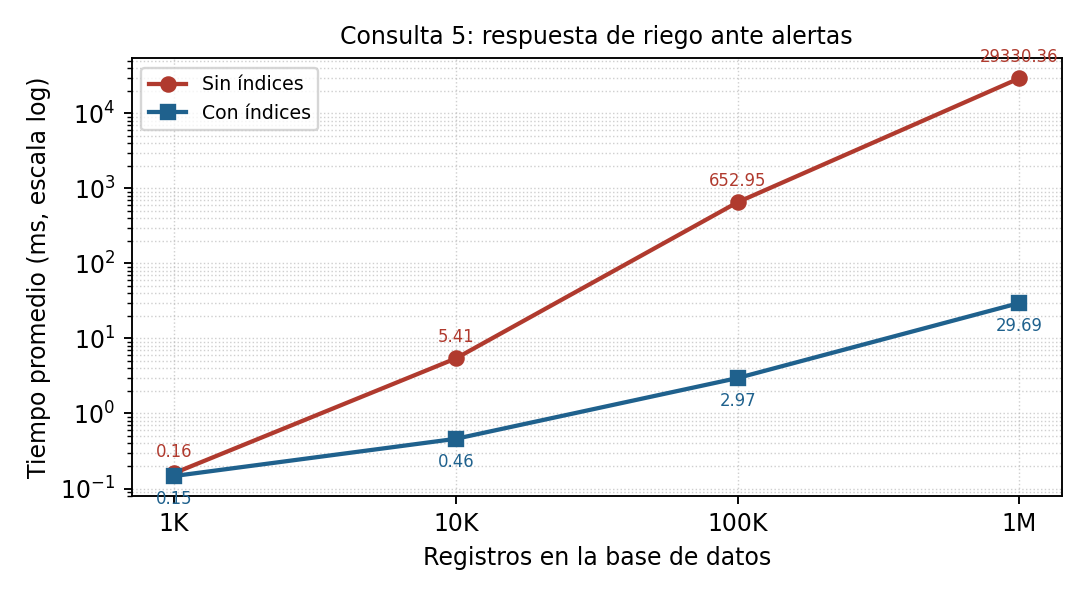
\includegraphics[width=0.78\textwidth]{figuras/consulta5.png}
\caption{Consulta 5: tiempo promedio por escenario.}
\end{figure}

\begin{table}[H]
\centering\small
\begin{tabular}{lrrrr}
\toprule
Escenario & Sin índices (ms) & Con índices (ms) & Relación sin/con & Filas devueltas \\
\midrule
1K & 0.160 & 0.147 & 1.09 & 1 \\
10K & 5.411 & 0.459 & 11.78 & 4 \\
100K & 652.95 & 2.968 & 220.01 & 8 \\
1M & 29\,330.36 & 29.69 & 987.82 & 12 \\
\bottomrule
\end{tabular}
\caption{Consulta 5: promedios y relación de mejora.}
\end{table}


Es la mejora más grande del experimento: con un millón de registros la consulta pasa de 29 segundos a 30 milisegundos, casi mil veces más rápida. Sin índice, la subconsulta correlacionada ejecuta un recorrido secuencial de \tb{Evento\_Riego} por cada una de las 7\,714 alertas y descarta en promedio unas 60\,000 filas en cada uno. Con índice, cada búsqueda es un \emph{Index Only Scan} sobre \tb{uq\_evento} que tarda alrededor de un microsegundo. La brecha crece con el volumen: 12 veces en 10\,000 registros, 220 veces en 100\,000 y casi mil en un millón.

\textbf{Plan de ejecución sin índices (1M)}
\begin{lstlisting}[style=plano]
Sort (actual time=29572.617..29572.626 rows=12 loops=1)
Sort Key: (round(((100.0 * (count(*) FILTER (WHERE (SubPlan 2)))::numeric) / (count(*))::numeric), 2))
Sort Method: quicksort  Memory: 25kB
->  GroupAggregate (actual time=2290.335..29572.571 rows=12 loops=1)
  Group Key: f.nombre
  Filter: (count(*) > 3)
  ->  Sort (actual time=350.841..355.686 rows=7714 loops=1)
    Sort Key: f.nombre
    Sort Method: quicksort  Memory: 614kB
    ->  Hash Join (actual time=343.289..349.062 rows=7714 loops=1)
      Hash Cond: (p.id_fundo = f.id_fundo)
      ->  Hash Join (actual time=0.871..5.670 rows=7714 loops=1)
        Hash Cond: (d.id_parcela = p.id_parcela)
        ->  Hash Join (actual time=0.735..4.518 rows=7714 loops=1)
          Hash Cond: (a.id_dispositivo = d.id_dispositivo)
          ->  Seq Scan on alerta a (actual time=0.009..2.694 rows=7714 loops=1)
            Filter: (((severidad)::text = ANY ('{Alta,Critica}'::text[])) AND ((tipo)::text = 'Humedad baja'::text))
            Rows Removed by Filter: 22286
          ->  Hash (actual time=0.715..0.716 rows=2800 loops=1)
            Buckets: 4096  Batches: 1  Memory Usage: 153kB
            ->  Seq Scan on dispositivo d (actual time=0.005..0.314 rows=2800 loops=1)
        ->  Hash (actual time=0.121..0.122 rows=600 loops=1)
          Buckets: 1024  Batches: 1  Memory Usage: 32kB
          ->  Seq Scan on parcela p (actual time=0.013..0.063 rows=600 loops=1)
      ->  Hash (actual time=342.406..342.407 rows=12 loops=1)
        Buckets: 1024  Batches: 1  Memory Usage: 9kB
        ->  Seq Scan on fundo f (actual time=342.375..342.382 rows=12 loops=1)
  SubPlan 1
   ->  Seq Scan on evento_riego er (actual time=1.859..1.859 rows=1 loops=7714)
     Filter: ((fecha_hora_inicio > a.fecha_hora) AND (id_parcela = d.id_parcela) AND (num_zona = d.num_zona) AND (fecha_hora_inicio <= (a.fecha_hora + '06:00:00'::interval)))
     Rows Removed by Filter: 60186
  SubPlan 2
   ->  Seq Scan on evento_riego er_1 (actual time=1.921..1.921 rows=1 loops=7714)
     Filter: ((fecha_hora_inicio > a.fecha_hora) AND (id_parcela = d.id_parcela) AND (num_zona = d.num_zona) AND (fecha_hora_inicio <= (a.fecha_hora + '06:00:00'::interval)))
     Rows Removed by Filter: 60186
Planning Time: 0.457 ms
Execution Time: 29574.874 ms
\end{lstlisting}

\textbf{Plan de ejecución con índices (1M)}
\begin{lstlisting}[style=plano]
Sort (actual time=28.026..28.031 rows=12 loops=1)
Sort Key: (round(((100.0 * (count(*) FILTER (WHERE (SubPlan 2)))::numeric) / (count(*))::numeric), 2))
Sort Method: quicksort  Memory: 25kB
->  GroupAggregate (actual time=7.819..28.018 rows=12 loops=1)
  Group Key: f.nombre
  Filter: (count(*) > 3)
  ->  Sort (actual time=6.343..6.802 rows=7714 loops=1)
    Sort Key: f.nombre
    Sort Method: quicksort  Memory: 614kB
    ->  Hash Join (actual time=0.718..4.859 rows=7714 loops=1)
      Hash Cond: (p.id_fundo = f.id_fundo)
      ->  Hash Join (actual time=0.703..3.764 rows=7714 loops=1)
        Hash Cond: (d.id_parcela = p.id_parcela)
        ->  Hash Join (actual time=0.580..2.580 rows=7714 loops=1)
          Hash Cond: (a.id_dispositivo = d.id_dispositivo)
          ->  Index Only Scan using idx_alerta_humedad_baja on alerta a (actual time=0.018..0.908 rows=7714 loops=1)
            Index Cond: (severidad = ANY ('{Alta,Critica}'::text[]))
            Heap Fetches: 0
          ->  Hash (actual time=0.556..0.557 rows=2800 loops=1)
            Buckets: 4096  Batches: 1  Memory Usage: 153kB
            ->  Seq Scan on dispositivo d (actual time=0.003..0.293 rows=2800 loops=1)
        ->  Hash (actual time=0.121..0.121 rows=600 loops=1)
          Buckets: 1024  Batches: 1  Memory Usage: 32kB
          ->  Seq Scan on parcela p (actual time=0.002..0.057 rows=600 loops=1)
      ->  Hash (actual time=0.011..0.011 rows=12 loops=1)
        Buckets: 1024  Batches: 1  Memory Usage: 9kB
        ->  Seq Scan on fundo f (actual time=0.004..0.006 rows=12 loops=1)
  SubPlan 1
   ->  Index Only Scan using uq_evento on evento_riego er (actual time=0.001..0.001 rows=1 loops=7714)
     Index Cond: ((id_parcela = d.id_parcela) AND (num_zona = d.num_zona) AND (fecha_hora_inicio > a.fecha_hora) AND (fecha_hora_inicio <= (a.fecha_hora + '06:00:00'::interval)))
     Heap Fetches: 0
  SubPlan 2
   ->  Index Only Scan using uq_evento on evento_riego er_1 (actual time=0.001..0.001 rows=1 loops=7714)
     Index Cond: ((id_parcela = d.id_parcela) AND (num_zona = d.num_zona) AND (fecha_hora_inicio > a.fecha_hora) AND (fecha_hora_inicio <= (a.fecha_hora + '06:00:00'::interval)))
     Heap Fetches: 0
Planning Time: 0.533 ms
Execution Time: 28.082 ms
\end{lstlisting}


\subsection{Análisis y Discusión}
\label{sec:discusion}

\begin{figure}[H]
\centering
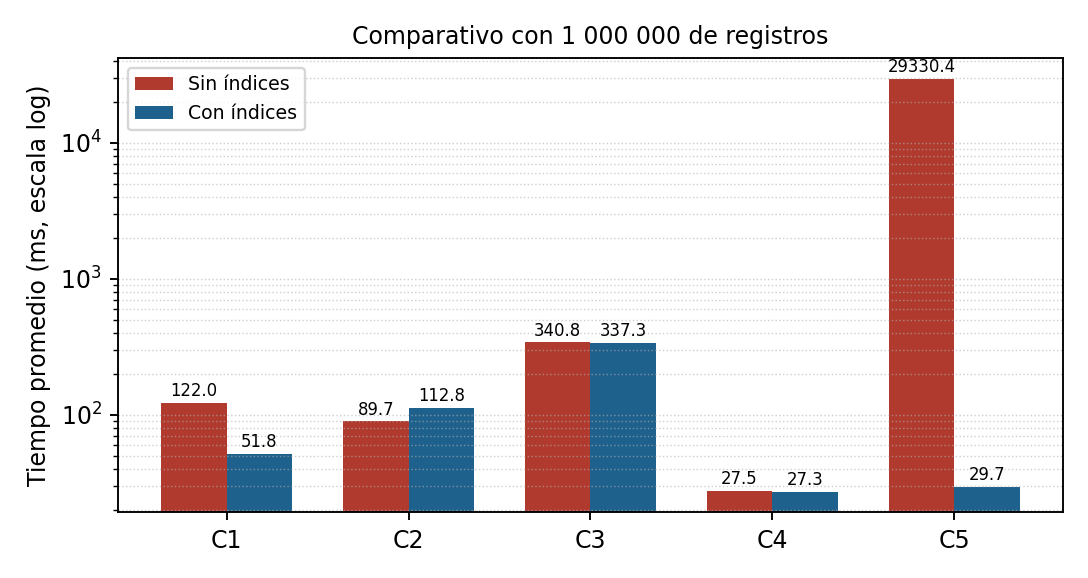
\includegraphics[width=0.78\textwidth]{figuras/comparativo1m.png}
\caption{Comparación de las cinco consultas con un millón de registros.}
\end{figure}

\begin{table}[H]
\centering\small
\begin{tabular}{lrrrr}
\toprule
Consulta & 1K & 10K & 100K & 1M \\
\midrule
C1 & 1.06 & 1.37 & 1.70 & 2.36 \\
C2 & 1.06 & 1.03 & 1.07 & 0.80 \\
C3 & 1.09 & 1.02 & 0.97 & 1.01 \\
C4 & 1.00 & 1.03 & 1.01 & 1.01 \\
C5 & 1.09 & 11.78 & 220.01 & 987.82 \\
\bottomrule
\end{tabular}
\caption{Relación entre el tiempo sin índices y con índices. Un valor mayor que 1 indica mejora.}\label{tab:resumen}
\end{table}


\textbf{Los índices no mejoran todo.} De las cinco consultas, dos mejoran de forma clara, dos no cambian y una empeora. De los nueve índices propuestos, el planificador solo eligió tres en el escenario de un millón (\tb{idx\_lectura\_fecha}, \tb{idx\_alerta\_humedad\_baja} e \tb{idx\_evento\_parcela\_fecha}), y el tercero hizo más lenta la consulta 2. Los otros seis ocupan espacio y encarecen las escrituras sin aportar nada a estas consultas. La Tabla~\ref{tab:planes} resume qué método de acceso usó el plan en cada escenario.

\begin{table}[H]
\centering\small
\resizebox{\textwidth}{!}{\begin{tabular}{llp{3.1cm}p{3.1cm}p{3.1cm}p{3.1cm}}
\toprule
Consulta & Índices & 1K & 10K & 100K & 1M \\
\midrule
C1 & sin & Seq & Seq & Seq & Seq paralelo \\
 & con & Index Only (idx\_lectura\_fecha) & Index Only (idx\_lectura\_fecha) & Index Only (idx\_lectura\_fecha) & Index Only (idx\_lectura\_fecha) \\
C2 & sin & Seq & Seq & Seq & Seq paralelo \\
 & con & Seq & Seq & Seq & Nested Loop + Index (idx\_evento\_parcela\_fecha) \\
C3 & sin & Seq & Seq & Seq & Seq paralelo \\
 & con & Seq & Seq & Seq & Seq paralelo \\
C4 & sin & Seq & Seq & Seq & Seq \\
 & con & Seq & Seq & Seq & Seq \\
C5 & sin & Seq & Seq & Seq & Seq \\
 & con & Index Only (uq\_evento) & Index Only (uq\_evento) & Index Only (uq\_evento) & Index Only (uq\_evento) \\
\bottomrule
\end{tabular}}
\caption{Método de acceso a la tabla principal de cada consulta (C1 y C3: lecturas; C2 y C5: riegos; C4: cosechas).}\label{tab:planes}
\end{table}


\textbf{Cuándo ayuda un índice.} Ayuda cuando la consulta necesita una fracción pequeña de una tabla grande (consulta 1, el último mes) o cuando debe repetir muchas búsquedas puntuales (consulta 5, una por alerta). No ayuda cuando la consulta lee casi toda la tabla (consultas 3 y 4) ni cuando la tabla es tan pequeña que cabe en pocas páginas, como \tb{Campania} con 1\,500 filas. En los escenarios de mil y diez mil registros casi no hay diferencias por la misma razón: todo cabe en memoria y cualquier plan termina en fracciones de milisegundo.

\textbf{El planificador puede equivocarse.} La consulta 2 muestra que un índice razonable puede empeorar el tiempo. El planificador elige con estimaciones de costo, y cuando la estimación falla, como con el \emph{Memoize} sin aciertos, el plan resultante es peor. Además, el efecto se invirtió entre escenarios: con 100\,000 registros el índice ayudaba un poco. Cada índice debe validarse con \tb{EXPLAIN ANALYZE} en un volumen representativo, no darse por bueno en teoría.

\textbf{Optimización lógica y física.} La consulta 5 repite la misma subconsulta \tb{EXISTS} en dos lugares, así que se evalúa dos veces por alerta. La reescribimos para evaluarla una sola vez dentro de una CTE (Tabla~\ref{tab:reescritura}).

\begin{table}[H]
\centering\small
\begin{tabular}{lrr}
\toprule
Versión de la consulta 5 & Sin índices (ms) & Con índices (ms) \\
\midrule
Original (EXISTS en dos lugares) & 29\,944.72 (5 it.) & 29.08 (5 it.) \\
CTE en línea & 29\,723.89 (5 it.) & 28.77 (5 it.) \\
CTE con \texttt{AS MATERIALIZED} & 15\,333.69 (3 it.) & 21.58 (5 it.) \\
\bottomrule
\end{tabular}
\caption{Efecto de reescribir la consulta 5 (1M). Las tres versiones devuelven exactamente las mismas filas.}\label{tab:reescritura}
\end{table}


La primera reescritura no mejoró nada, y la causa es una característica de PostgreSQL que conviene conocer: desde la versión 12, una CTE que se usa una sola vez se incrusta en la consulta principal, y al hacerlo la expresión \tb{EXISTS} volvió a aparecer en los dos agregados. El plan lo confirma: siguen existiendo dos subconsultas y no aparece ningún \emph{CTE Scan}. Al declarar la CTE como \tb{MATERIALIZED}, la subconsulta se evalúa una sola vez y el tiempo sin índices baja a la mitad. Es una mejora real, pero pequeña frente al índice: reescribir divide el tiempo entre dos y el índice lo divide entre mil. Lo ideal es combinar ambas cosas.

\begin{lstlisting}[style=sql, title={03c\_consulta5\_materializada.sql}]
-- Consulta 5 reescrita con AS MATERIALIZED: impide que PostgreSQL incruste la
-- CTE y garantiza que el EXISTS se evalue una sola vez por alerta.
WITH evaluadas AS MATERIALIZED (
    SELECT f.nombre AS fundo,
           EXISTS (
               SELECT 1
               FROM Evento_Riego er
               WHERE er.id_parcela = d.id_parcela
                 AND er.num_zona   = d.num_zona
                 AND er.fecha_hora_inicio >  a.fecha_hora
                 AND er.fecha_hora_inicio <= a.fecha_hora + INTERVAL '6 hours'
           ) AS con_riego
    FROM Alerta       a
    JOIN Dispositivo  d ON d.id_dispositivo = a.id_dispositivo
    JOIN Parcela      p ON p.id_parcela = d.id_parcela
    JOIN Fundo        f ON f.id_fundo   = p.id_fundo
    WHERE a.tipo = 'Humedad baja'
      AND a.severidad IN ('Alta','Critica')
)
SELECT fundo,
       COUNT(*)                                                    AS alertas,
       COUNT(*) FILTER (WHERE con_riego)                           AS atendidas_con_riego,
       ROUND(100.0 * COUNT(*) FILTER (WHERE con_riego) / COUNT(*), 2) AS pct_respuesta
FROM evaluadas
GROUP BY fundo
HAVING COUNT(*) > 3
ORDER BY pct_respuesta ASC;
\end{lstlisting}


\textbf{Resumen práctico.} Para esta base recomendamos conservar \tb{idx\_lectura\_fecha} (o su versión BRIN si el espacio importa) e \tb{idx\_alerta\_humedad\_baja}, y retirar los otros siete. En particular, \tb{idx\_lectura\_disp\_humedad} ocupa 24~MB, nunca se usa y encarece cada actualización de humedad.

\subsection{Complejidad operacional por encima del millón de registros}
\label{sec:extra}

\textbf{Cómo crece cada consulta.} La Tabla~\ref{tab:crecimiento} muestra cuántas veces aumenta el tiempo cuando los datos se multiplican por diez. Si el factor es cercano a 10, el crecimiento es lineal; si se acerca a 100, es cuadrático. El exponente $b$ resume el último tramo: el tiempo crece como $n^b$.

\begin{table}[H]
\centering\small
\begin{tabular}{llrrrr}
\toprule
Consulta & Índices & 1K$\to$10K & 10K$\to$100K & 100K$\to$1M & Exponente $b$ \\
\midrule
C1 & sin & 3.7 & 8.0 & 12.6 & 1.10 \\
 & con & 2.9 & 6.4 & 9.1 & 0.96 \\
C2 & sin & 4.3 & 8.3 & 10.4 & 1.02 \\
 & con & 4.4 & 7.9 & 14.0 & 1.15 \\
C3 & sin & 7.0 & 10.2 & 11.3 & 1.05 \\
 & con & 7.5 & 10.7 & 10.8 & 1.03 \\
C4 & sin & 3.1 & 5.9 & 7.2 & 0.86 \\
 & con & 3.0 & 6.0 & 7.2 & 0.86 \\
C5 & sin & 33.9 & 120.7 & 44.9 & 1.65 \\
 & con & 3.1 & 6.5 & 10.0 & 1.00 \\
\bottomrule
\end{tabular}
\caption{Factor de crecimiento del tiempo cuando los datos se multiplican por diez.}\label{tab:crecimiento}
\end{table}


Casi todas las consultas crecen de forma lineal ($b \approx 1$), lo que corresponde a recorridos completos de tabla con uniones hash: el costo es proporcional al número de filas. La excepción es la consulta 5 sin índice, con exponentes entre 1.6 y 2.1. La razón es que el número de alertas y el de riegos crecen a la vez, y por cada alerta se recorre la tabla de riegos: el costo es $O(A \cdot E)$, que en la práctica es cuadrático. Con el índice, cada búsqueda cuesta $O(\log E)$ y el total queda en $O(A \log E)$, casi lineal, como confirma el exponente de 1.0.

\textbf{Proyección.} Si extrapolamos esos exponentes, con diez millones de registros la consulta 5 sin índice pasaría de 30 segundos a entre 20 y 60 minutos, mientras que con índice rondaría los 300~ms. La consulta 1 sin índice subiría a alrededor de un segundo y medio. Son estimaciones gruesas, porque al crecer la base dejaría de caber en memoria y aparecerían lecturas de disco que hoy no existen, pero el orden de magnitud basta para ver que los recorridos completos dejan de ser una opción.

\textbf{Volumen real esperado.} Con los 2\,200 sensores reportando cada 15 minutos, la tabla de lecturas recibiría unos 77.1 millones de filas al año (alrededor de 13.2 GB con los índices actuales). El ritmo de escritura no es el problema: equivale a unas 2.4 lecturas por segundo, y en la prueba de escritura insertamos 20\,000 lecturas en 238~ms, unas 84\,000 por segundo con todos los índices. Aunque registrar fila por fila con el trigger de alertas es mucho más lento que una inserción masiva, el margen es de varios órdenes de magnitud. El problema está en las consultas analíticas sobre años de historia. Incluso la consulta 1 con índice escala con el tamaño de la ventana consultada: con la frecuencia real, un mes tendría unos 6.3 millones de lecturas, y leerlas por índice tomaría varios segundos.

\textbf{¿Es suficiente la arquitectura cliente-servidor?} Para el volumen de esta empresa, sí, siempre que el servidor se organice para ese crecimiento. En orden de prioridad:

\begin{enumerate}[leftmargin=1.6em,itemsep=0.15em]
\item \textbf{Particionamiento por rango de fecha.} Dividir \tb{Lectura\_Suelo} en particiones mensuales con el particionamiento declarativo de PostgreSQL. Una consulta del último mes solo toca una partición (\emph{partition pruning}), y las particiones antiguas pueden archivarse o desconectarse sin borrar fila por fila.
\item \textbf{BRIN por partición.} Como los datos llegan en orden cronológico, un BRIN sobre la fecha cuesta kilobytes en lugar de megabytes y casi iguala al B+ tree, como medimos.
\item \textbf{Agregados materializados.} Una vista materializada con el resumen diario por sensor (promedio, mínimo, máximo y conteo), refrescada cada noche. Las consultas 1 y 3 leerían unas 2\,200 filas por día en lugar de 211\,000 lecturas.
\item \textbf{Réplica de lectura.} Una réplica por \emph{streaming replication} para los reportes de gerencia, de modo que las consultas pesadas no compitan con la ingesta.
\item \textbf{Extensiones especializadas.} Si el volumen creciera mucho más, TimescaleDB añade a PostgreSQL particionamiento automático, compresión y agregados continuos para series de tiempo, sin salir del modelo relacional.
\end{enumerate}

El modelo cliente-servidor dejaría de ser suficiente en otro escenario: una plataforma que atienda a miles de fundos de distintas empresas, con miles de millones de filas por año, alta disponibilidad entre regiones o análisis que recorran terabytes. Ahí el lado del servidor tendría que convertirse en un clúster distribuido o apoyarse en un almacén columnar para la analítica. Aun así, los clientes seguirían hablando con un servicio; lo que cambia es que ese servicio ya no es una sola máquina.

% ================================================================== 6
\section{Conclusiones}

\begin{enumerate}[leftmargin=1.6em,itemsep=0.25em]
\item El modelo cubre el dominio con una especialización total y disjunta, dos entidades débiles y una relación ternaria. El esquema resultante está en tercera forma normal. La única tabla que no cumple FNBC (\tb{Evento\_Riego}) se dejó así a propósito para preservar dependencias, y la dependencia se controla con un trigger.
\item Llevar las reglas del negocio a la base de datos funcionó. Restricciones, procedimientos y triggers rechazaron todas las operaciones inválidas de las pruebas, y las verificaciones de consistencia encontraron errores del generador que habrían contaminado el experimento.
\item Los índices no son una mejora universal. Solo dos de las cinco consultas se aceleraron (2.4 y casi mil veces), dos no cambiaron y una se volvió 26~\% más lenta. Solo tres de los nueve índices propuestos llegaron a usarse.
\item La mayor ganancia aparece en las subconsultas correlacionadas: el índice convierte un costo cuadrático en uno casi lineal, y la diferencia crece con el volumen.
\item Para series de tiempo guardadas en orden de llegada, un BRIN ofrece casi el mismo beneficio que un B+ tree con una fracción mínima del espacio. En un sistema IoT que crece de forma indefinida, esa diferencia pesa.
\item Todo índice cuesta en escritura, entre 12 y 75~\% en nuestras pruebas, y el peor caso aparece al actualizar columnas incluidas en índices. En tablas que reciben datos de forma continua, cada índice debe justificarse con mediciones.
\item La optimización lógica también cuenta, pero hay que verificarla. Reescribir la consulta 5 no sirvió hasta forzar la materialización de la CTE; después, redujo el tiempo a la mitad.
\item La arquitectura cliente-servidor basta para el volumen previsto si se combina con particionamiento por fecha, índices BRIN y agregados materializados. Las alternativas distribuidas solo se justificarían con una escala varios órdenes de magnitud mayor.
\end{enumerate}

% ================================================================== 7
\section{Anexos}

\subsection{Video de demostración}

Video con la base de un millón de registros, ejecutando las consultas con y sin índices: \enlaceVideo

Los comandos que se muestran en el video son los siguientes:

\begin{lstlisting}
-- 1. Restaurar el respaldo (desde la terminal)
--    createdb agro1m
--    pg_restore -d agro1m agro_1M.dump
-- 2. Comprobar el volumen
SELECT (SELECT count(*) FROM Lectura_Suelo) AS lecturas,
       (SELECT count(*) FROM Evento_Riego)  AS riegos,
       (SELECT count(*) FROM Alerta)        AS alertas;
-- 3. Consulta 5 sin indices
SET enable_indexscan = OFF; SET enable_bitmapscan = OFF; SET enable_indexonlyscan = OFF;
EXPLAIN ANALYZE <consulta 5>;
-- 4. Consulta 5 con indices
SET enable_indexscan = ON; SET enable_bitmapscan = ON; SET enable_indexonlyscan = ON;
EXPLAIN ANALYZE <consulta 5>;
\end{lstlisting}

\subsection{Respaldos de la base de datos}

Los cuatro respaldos se generaron con \tb{pg\_dump} en formato personalizado y compresión nivel 6: \enlaceDumps

\begin{table}[H]
\centering\small
\begin{tabular}{lrr}
\toprule
Archivo & Registros & Tamaño (MB) \\
\midrule
\texttt{agro\_1K.dump} & 1\,000 & 0.13 \\
\texttt{agro\_10K.dump} & 10\,000 & 0.25 \\
\texttt{agro\_100K.dump} & 100\,000 & 1.47 \\
\texttt{agro\_1M.dump} & 1\,000\,000 & 13.74 \\
\bottomrule
\end{tabular}
\caption{Respaldos entregados.}\label{tab:dumps}
\end{table}


Para restaurar uno de ellos: \tb{createdb agro1m} y luego \tb{pg\_restore -d agro1m agro\_1M.dump}.

\subsection{Scripts del proyecto}

Carpeta con todos los scripts: \enlaceRepositorio

\begin{table}[H]
\centering\small
\begin{tabularx}{\textwidth}{>{\raggedright\arraybackslash}p{5.4cm}X}
\toprule
\textbf{Archivo} & \textbf{Contenido} \\
\midrule
\tb{sql/01\_ddl.sql} & Creación de las 18 tablas con sus restricciones. \\
\tb{sql/01b\_comentarios.sql} & Documentación de tablas y columnas (fuente del diccionario). \\
\tb{sql/02\_vistas\_procedimientos\_triggers.sql} & Vistas, procedimientos, funciones y triggers. \\
\tb{sql/03\_consultas.sql} & Las cinco consultas del experimento. \\
\tb{sql/03b\_consulta5\_reescrita.sql}, \tb{03c\ldots} & Reescrituras de la consulta 5. \\
\tb{sql/04\_indices.sql} & Los nueve índices de optimización. \\
\tb{sql/05\_roles.sql} & Roles y permisos (opcional). \\
\tb{sql/06\_pruebas.sql} & Pruebas de procedimientos y triggers. \\
\tb{sql/07\_verificacion.sql} & Verificación de consistencia posterior a la carga. \\
\tb{scripts/generar\_datos.py} & Generador de datos sintéticos. \\
\tb{scripts/ejecutar\_todo.py} & Orquestador: carga, experimento y gráficos. \\
\tb{scripts/experimento.py} & Mediciones, reanudables por tramos. \\
\tb{scripts/graficos.py} & Figuras del informe. \\
\tb{scripts/construir\_informe.py} & Genera las tablas y listados de este informe desde los resultados. \\
\bottomrule
\end{tabularx}
\caption{Archivos entregados.}
\end{table}

\subsection{Generador de datos}
\label{sec:generador}

\begin{lstlisting}[style=py]
#!/usr/bin/env python3
# -*- coding: utf-8 -*-
"""
Generador de datos sinteticos - Agricultura de Precision y Sensores IoT
Curso: Base de Datos I (CS2041) - Laboratorio 14 - 2026-2

Uso:  python generar_datos.py <total_registros> <carpeta_salida>
Ej.:  python generar_datos.py 1000000 ../data/1M

Produce un CSV por tabla. La suma de filas de todas las tablas es exactamente
<total_registros>; la tabla Lectura_Suelo absorbe el saldo.
Los parametros agronomicos (rangos optimos, rendimientos, caudales) se tomaron
de valores de referencia publicos para la agricultura peruana.
"""
import csv, os, random, sys
from datetime import date, datetime, timedelta

SEED = 20251047
INICIO_SERIE = datetime(2026, 1, 1)
FIN_SERIE = datetime(2026, 9, 15, 23, 59)
VENTANA_SEG = int((FIN_SERIE - INICIO_SERIE).total_seconds())
REF = date(2026, 9, 20)                 # fecha de corte del caso de estudio
NULO = ""                               # NULL para COPY ... NULL ''

# departamento, provincia, distrito, lat, lon, temperatura media del suelo (C)
DEPARTAMENTOS = [
    ("Ica", "Ica", "Salas Guadalupe", -14.07, -75.73, 23),
    ("La Libertad", "Viru", "Chao", -8.48, -78.72, 22),
    ("Lambayeque", "Chiclayo", "Motupe", -6.15, -79.72, 24),
    ("Piura", "Sullana", "Bellavista", -4.90, -80.69, 26),
    ("Arequipa", "Caylloma", "Majes", -16.33, -72.19, 18),
    ("Ancash", "Casma", "Comandante Noel", -9.47, -78.30, 21),
    ("Lima", "Huaral", "Chancay", -11.57, -77.27, 19),
    ("Junin", "Chanchamayo", "Perene", -10.95, -75.22, 24),
    ("San Martin", "Lamas", "Tabalosos", -6.42, -76.63, 26),
    ("Cusco", "La Convencion", "Echarate", -12.77, -72.57, 24),
    ("Cajamarca", "Jaen", "Bellavista", -5.67, -78.67, 25),
    ("Amazonas", "Utcubamba", "Bagua Grande", -5.76, -78.44, 26),
]
NOMBRES_FUNDO = ["Santa Rita", "El Algarrobal", "Los Olivares", "Pampa Verde",
                 "San Jacinto", "La Huaca", "Tierra Nueva", "El Mirador",
                 "Valle Alto", "Sol de Oro", "Las Lomas", "Buenaventura"]

# nombre, cientifico, ciclo, hmin, hmax, phmin, phmax, ce_max, t/ha, S/ por kg
CULTIVOS = [
    ("Esparrago", "Asparagus officinalis", 270, 55, 75, 6.5, 7.5, 3.0, 11, 5.5),
    ("Arandano", "Vaccinium corymbosum", 365, 60, 80, 4.5, 5.5, 1.5, 14, 12.0),
    ("Palto Hass", "Persea americana", 420, 55, 70, 5.5, 7.0, 2.0, 12, 6.0),
    ("Uva de mesa", "Vitis vinifera", 300, 45, 65, 6.0, 7.5, 2.5, 25, 7.0),
    ("Mango Kent", "Mangifera indica", 330, 50, 70, 5.5, 7.5, 2.0, 16, 2.5),
    ("Quinua", "Chenopodium quinoa", 150, 40, 60, 6.0, 8.0, 4.0, 2, 6.0),
    ("Papa Canchan", "Solanum tuberosum", 120, 60, 80, 5.0, 6.5, 2.0, 22, 1.2),
    ("Maiz amarillo", "Zea mays", 140, 55, 75, 5.8, 7.0, 3.5, 9, 1.1),
    ("Cacao", "Theobroma cacao", 400, 65, 85, 5.0, 7.5, 1.5, 1, 9.0),
    ("Cafe Caturra", "Coffea arabica", 390, 60, 80, 4.5, 6.0, 1.5, 1, 14.0),
    ("Alcachofa", "Cynara scolymus", 180, 60, 75, 6.0, 7.5, 3.0, 18, 2.2),
    ("Pimiento piquillo", "Capsicum annuum", 130, 55, 70, 6.0, 7.0, 2.5, 28, 2.8),
]
# cultivos aptos por departamento (se evita, por ejemplo, cacao en Ica)
APTOS = {
    "Ica": ["Esparrago", "Uva de mesa", "Palto Hass", "Arandano", "Pimiento piquillo"],
    "La Libertad": ["Esparrago", "Arandano", "Palto Hass", "Alcachofa", "Pimiento piquillo"],
    "Lambayeque": ["Mango Kent", "Palto Hass", "Maiz amarillo", "Uva de mesa"],
    "Piura": ["Mango Kent", "Uva de mesa", "Arandano", "Maiz amarillo"],
    "Arequipa": ["Quinua", "Alcachofa", "Papa Canchan", "Palto Hass"],
    "Ancash": ["Esparrago", "Palto Hass", "Maiz amarillo", "Mango Kent"],
    "Lima": ["Palto Hass", "Maiz amarillo", "Papa Canchan", "Alcachofa"],
    "Junin": ["Cafe Caturra", "Cacao", "Maiz amarillo"],
    "San Martin": ["Cacao", "Cafe Caturra", "Maiz amarillo"],
    "Cusco": ["Cafe Caturra", "Cacao"],
    "Cajamarca": ["Cafe Caturra", "Cacao", "Maiz amarillo"],
    "Amazonas": ["Cafe Caturra", "Cacao", "Maiz amarillo"],
}

INSUMOS = [  # nombre, tipo, unidad, costo, carencia
    ("Nitrato de amonio 33.5", "Fertilizante", "kg", 3.20, 0),
    ("Sulfato de potasio", "Fertilizante", "kg", 4.80, 0),
    ("Fosfato diamonico", "Fertilizante", "kg", 4.10, 0),
    ("Acido fosforico 85%", "Fertilizante", "L", 6.50, 0),
    ("Yeso agricola", "Enmienda", "kg", 0.90, 0),
    ("Azufre micronizado", "Enmienda", "kg", 2.30, 3),
    ("Mancozeb 80 WP", "Fungicida", "kg", 28.00, 7),
    ("Azoxistrobina 25 SC", "Fungicida", "L", 95.00, 14),
    ("Abamectina 1.8 EC", "Insecticida", "L", 78.00, 7),
    ("Imidacloprid 35 SC", "Insecticida", "L", 64.00, 21),
    ("Extracto de algas", "Bioestimulante", "L", 42.00, 0),
    ("Aminoacidos libres 20%", "Bioestimulante", "L", 55.00, 0),
    ("Quelato de hierro EDDHA", "Fertilizante", "kg", 38.00, 0),
    ("Cal dolomita", "Enmienda", "kg", 0.65, 0),
    ("Bacillus subtilis WP", "Fungicida", "kg", 61.00, 0),
]
DOSIS = {"Fertilizante": (25, 400), "Enmienda": (100, 900), "Fungicida": (0.3, 6),
         "Insecticida": (0.2, 4), "Bioestimulante": (1, 15)}
METODOS = {"Fertilizante": ["Fertirriego", "Al suelo"], "Enmienda": ["Al suelo"],
           "Fungicida": ["Foliar", "Drench"], "Insecticida": ["Foliar", "Drench"],
           "Bioestimulante": ["Foliar", "Fertirriego"]}

# tipo de sensor -> variables que mide y modelos comerciales compatibles
SENSORES = {
    "Humedad": ({"hum", "temp"}, [("SMT100", "TRUEBNER"), ("Watermark 200SS", "Irrometer")]),
    "Multiparametro": ({"hum", "temp", "ph", "ce"}, [("JXBS-3001", "JXCT")]),
    "Conductividad": ({"hum", "temp", "ce"}, [("TEROS 12", "METER Group"),
                                              ("HydraProbe", "Stevens Water")]),
    "pH": ({"ph", "temp"}, [("Sonda pH de suelo", "JXCT")]),
    "Temperatura": ({"temp"}, [("107", "Campbell Scientific")]),
}
PESOS_SENSOR = {"Humedad": 35, "Multiparametro": 40, "Conductividad": 10, "pH": 10,
                "Temperatura": 5}
UNIDAD = {"Humedad": "%", "Multiparametro": "mixto", "Conductividad": "dS/m",
          "pH": "pH", "Temperatura": "C"}
CONTROLADORES = [("NMC-Pro", "Netafim"), ("ACC2", "Hunter"),
                 ("ESP-LXME2", "Rain Bird"), ("GSI", "Galcon")]

NOMBRES = ["Juan", "Maria", "Jose", "Rosa", "Carlos", "Ana", "Luis", "Carmen", "Miguel",
           "Elena", "Pedro", "Silvia", "Jorge", "Lucia", "Victor", "Gladys", "Raul", "Martha",
           "Cesar", "Nancy", "Felipe", "Yolanda", "Hugo", "Teresa", "Marco", "Julia", "Oscar",
           "Beatriz", "Angel", "Pilar"]
APELLIDOS = ["Quispe", "Mamani", "Flores", "Rojas", "Vasquez", "Huaman", "Chavez", "Ramos",
             "Castillo", "Torres", "Vargas", "Espinoza", "Salazar", "Cordova", "Tapia",
             "Ccahuana", "Zevallos", "Palomino", "Bustamante", "Aguirre", "Nunez", "Paredes",
             "Guzman", "Lescano", "Meza"]
ROLES = ["Tecnico de campo", "Ingeniero agronomo", "Operador de riego", "Supervisor"]
SUELOS = ["Arenoso", "Franco", "Franco arenoso", "Franco arcilloso", "Arcilloso"]
TIPOS_RIEGO = ["Goteo", "Aspersion", "Microaspersion", "Gravedad tecnificada"]
FUENTES = ["Pozo", "Canal", "Reservorio", "Rio"]
VALVULAS = ["Solenoide", "Hidraulica", "Manual motorizada"]
CATEGORIAS = ["Primera", "Segunda", "Tercera", "Descarte"]

PERFILES = {
    1_000: dict(fundo=3, cultivo=8, insumo=10, operario=12, parcela=15, zona=40,
                campania=25, sensor=35, controlador=10, evento=120, alerta=30,
                cosecha=40, aplicacion=40, mantenimiento=20),
    10_000: dict(fundo=5, cultivo=10, insumo=12, operario=40, parcela=50, zona=150,
                 campania=90, sensor=130, controlador=40, evento=1_200, alerta=300,
                 cosecha=350, aplicacion=400, mantenimiento=150),
    100_000: dict(fundo=8, cultivo=12, insumo=15, operario=150, parcela=200, zona=700,
                  campania=400, sensor=620, controlador=180, evento=12_000, alerta=3_000,
                  cosecha=3_000, aplicacion=4_000, mantenimiento=1_200),
    1_000_000: dict(fundo=12, cultivo=12, insumo=15, operario=400, parcela=600, zona=2_400,
                    campania=1_500, sensor=2_200, controlador=600, evento=120_000,
                    alerta=30_000, cosecha=25_000, aplicacion=40_000, mantenimiento=8_000),
}


def w(carpeta, nombre, cabecera, filas):
    with open(os.path.join(carpeta, nombre + ".csv"), "w", newline="", encoding="utf-8") as fh:
        esc = csv.writer(fh)
        esc.writerow(cabecera)
        esc.writerows(filas)
    return len(filas)


def ts(dt):
    return dt.strftime("%Y-%m-%d %H:%M:%S")


def instante():
    t = INICIO_SERIE + timedelta(seconds=random.randint(0, VENTANA_SEG))
    return t.replace(second=0, microsecond=0)


def generar(total, carpeta):
    random.seed(SEED + total)
    os.makedirs(carpeta, exist_ok=True)
    p = PERFILES[total]
    p["sistema"] = p["parcela"]          # un sistema de riego por parcela
    n = {}

    # ---------------------------------------------------------- FUNDO
    fundos = []
    for i in range(1, p["fundo"] + 1):
        dep, prov, dist, lat, lon, _ = DEPARTAMENTOS[i - 1]
        fundos.append([i, NOMBRES_FUNDO[i - 1], dep, prov, dist,
                       round(random.uniform(60, 900), 2),
                       round(lat + random.uniform(-0.2, 0.2), 6),
                       round(lon + random.uniform(-0.2, 0.2), 6),
                       (date(2019, 1, 1) + timedelta(days=random.randint(0, 2000))).isoformat()])
    n["Fundo"] = w(carpeta, "fundo", ["id_fundo", "nombre", "departamento", "provincia",
                   "distrito", "area_total_ha", "latitud", "longitud", "fecha_registro"], fundos)
    dep_fundo = {f[0]: f[2] for f in fundos}
    temp_dep = {d[0]: d[5] for d in DEPARTAMENTOS}

    # -------------------------------------------------------- CULTIVO
    cultivos = [[i] + list(c[:8]) for i, c in enumerate(CULTIVOS[:p["cultivo"]], start=1)]
    n["Cultivo"] = w(carpeta, "cultivo", ["id_cultivo", "nombre_comun", "nombre_cientifico",
                     "ciclo_dias", "humedad_optima_min", "humedad_optima_max", "ph_optimo_min",
                     "ph_optimo_max", "ce_maxima_ds_m"], cultivos)
    info = {i: CULTIVOS[i - 1] for i in range(1, p["cultivo"] + 1)}
    id_por_nombre = {CULTIVOS[i - 1][0]: i for i in info}

    # --------------------------------------------------------- INSUMO
    insumos = [[i] + list(x) for i, x in enumerate(INSUMOS[:p["insumo"]], start=1)]
    n["Insumo"] = w(carpeta, "insumo", ["id_insumo", "nombre", "tipo", "unidad",
                    "costo_unitario", "periodo_carencia_dias"], insumos)
    tipo_insumo = {x[0]: x[2] for x in insumos}

    # ------------------------------------------------------- OPERARIO
    dnis, operarios = set(), []
    for i in range(1, p["operario"] + 1):
        while True:
            d = str(random.randint(10000000, 79999999))
            if d not in dnis:
                dnis.add(d)
                break
        tel = NULO if random.random() < 0.08 else "9" + str(random.randint(10000000, 99999999))
        operarios.append([i, d, random.choice(NOMBRES), random.choice(APELLIDOS),
                          random.choice(ROLES), tel, random.randint(1, p["fundo"]),
                          (date(2018, 1, 1) + timedelta(days=random.randint(0, 2800))).isoformat()])
    n["Operario"] = w(carpeta, "operario", ["id_operario", "dni", "nombre", "apellido", "rol",
                      "telefono", "id_fundo", "fecha_ingreso"], operarios)

    # -------------------------------------------------------- PARCELA
    parcelas, cont = [], {}
    for i in range(1, p["parcela"] + 1):
        f = random.randint(1, p["fundo"])
        cont[f] = cont.get(f, 0) + 1
        parcelas.append([i, f, "P-%03d" % cont[f], round(random.uniform(1.5, 35.0), 2),
                         random.choice(SUELOS), round(random.uniform(0, 12), 1),
                         (date(2020, 1, 1) + timedelta(days=random.randint(0, 1800))).isoformat()])
    n["Parcela"] = w(carpeta, "parcela", ["id_parcela", "id_fundo", "codigo_parcela", "area_ha",
                     "tipo_suelo", "pendiente_pct", "fecha_habilitacion"], parcelas)
    area = {r[0]: float(r[3]) for r in parcelas}
    fundo_parcela = {r[0]: r[1] for r in parcelas}

    # ---------------------------------------------------- ZONA_MANEJO
    zonas, zxp = [], {}
    for idp in range(1, p["parcela"] + 1):
        zxp[idp] = [1]
        zonas.append([idp, 1, round(area[idp] / 2, 2), "Zona de manejo 1"])
    while len(zonas) < p["zona"]:
        idp = random.randint(1, p["parcela"])
        k = len(zxp[idp]) + 1
        if k > 8:
            continue
        zxp[idp].append(k)
        zonas.append([idp, k, round(max(0.2, area[idp] / (k + 1)), 2), "Zona de manejo %d" % k])
    n["Zona_Manejo"] = w(carpeta, "zona_manejo", ["id_parcela", "num_zona", "area_ha",
                         "descripcion"], zonas)
    lista_zonas = [(z[0], z[1]) for z in zonas]

    # -------------------------------------------------- SISTEMA_RIEGO
    # caudal de 15 a 180 m3/h, coherente con riego sectorizado de 1.5 a 35 ha
    sistemas, sis_parcela, caudal = [], {}, {}
    for i in range(1, p["sistema"] + 1):
        c = round(random.uniform(15000, 180000), 2)
        sistemas.append([i, i, random.choice(TIPOS_RIEGO), c, random.choice(FUENTES),
                         (date(2021, 1, 1) + timedelta(days=random.randint(0, 1500))).isoformat(),
                         "Operativo" if random.random() > 0.07 else "Averiado"])
        sis_parcela[i] = i
        caudal[i] = c
    n["Sistema_Riego"] = w(carpeta, "sistema_riego", ["id_sistema", "id_parcela", "tipo",
                           "caudal_nominal_lph", "fuente_agua", "fecha_instalacion", "estado"],
                           sistemas)

    # ------------------------------------------------------- CAMPANIA
    # Cadenas hacia atras desde REF: la primera campania de cada parcela es la
    # vigente y las anteriores se encadenan sin solaparse.
    campanias, cursor = [], {}
    i, idp = 0, 0
    while i < p["campania"]:
        idp = idp % p["parcela"] + 1
        dep = dep_fundo[fundo_parcela[idp]]
        aptos = [id_por_nombre[c] for c in APTOS[dep] if c in id_por_nombre] or list(info)
        idc = random.choice(aptos)
        ciclo = info[idc][2]
        if idp not in cursor:
            siembra = REF - timedelta(days=int(ciclo * random.uniform(0.15, 0.85)))
            estado = "En curso" if random.random() > 0.10 else "Perdida"
        else:
            fin_prev = cursor[idp] - timedelta(days=random.randint(10, 60))
            siembra = fin_prev - timedelta(days=ciclo)
            estado = "Cerrada" if random.random() > 0.08 else "Perdida"
        fin = siembra + timedelta(days=ciclo)
        cursor[idp] = siembra
        i += 1
        campanias.append([i, idp, idc, siembra.isoformat(), fin.isoformat(),
                          random.choice([1200, 1600, 2500, 3300, 5000, 8000, 62500]), estado, 0])
    n["Campania"] = w(carpeta, "campania", ["id_campania", "id_parcela", "id_cultivo",
                      "fecha_siembra", "fecha_fin_estimada", "densidad_plantas_ha", "estado",
                      "rendimiento_kg_ha"], campanias)
    cultivo_vigente = {c[1]: c[2] for c in campanias if c[6] == "En curso"}

    # ------------------------------------------ DISPOSITIVO Y SUBCLASES
    n_disp = p["sensor"] + p["controlador"]
    disp, sens, ctrl, tipo_de = [], [], [], {}
    for i in range(1, n_disp + 1):
        idp, nz = lista_zonas[(i - 1) % len(lista_zonas)]
        if i <= p["sensor"]:
            t = random.choices(list(PESOS_SENSOR), weights=list(PESOS_SENSOR.values()))[0]
            modelo, fab = random.choice(SENSORES[t][1])
            tipo_de[i] = t
            sens.append([i, t, random.choice([10, 20, 30, 40, 60]),
                         random.choice([5, 10, 15, 30, 60]), UNIDAD[t], NULO, NULO])
        else:
            modelo, fab = random.choice(CONTROLADORES)
            ctrl.append([i, idp, round(random.uniform(4, 50), 2), random.choice(VALVULAS)])
        disp.append([i, "SN-%07d" % (400000 + i), modelo, fab,
                     (date(2023, 1, 1) + timedelta(days=random.randint(0, 900))).isoformat(),
                     "Activo" if random.random() > 0.06 else
                     random.choice(["Mantenimiento", "Inactivo"]), idp, nz])
    n["Dispositivo"] = w(carpeta, "dispositivo", ["id_dispositivo", "codigo_serie", "modelo",
                         "fabricante", "fecha_instalacion", "estado", "id_parcela", "num_zona"],
                         disp)
    n["Sensor"] = w(carpeta, "sensor", ["id_dispositivo", "tipo_sensor", "profundidad_cm",
                    "frecuencia_min", "unidad_medida", "rango_min", "rango_max"], sens)
    n["Controlador"] = w(carpeta, "controlador", ["id_dispositivo", "id_sistema",
                         "caudal_max_lps", "tipo_valvula"], ctrl)
    zona_de = {d[0]: (d[6], d[7]) for d in disp}

    # -------------------------------------------------- LECTURA_SUELO
    n_lect = total - sum(n.values()) - p["evento"] - p["alerta"] - p["cosecha"] \
        - p["aplicacion"] - p["mantenimiento"]
    assert n_lect > 0, "perfil mal dimensionado"
    con_cultivo = sorted(cultivo_vigente) or list(range(1, p["parcela"] + 1))
    secas = set(random.sample(con_cultivo, max(1, int(len(con_cultivo) * 0.22))))
    lecturas, vistos, cand_hum, cand_bat = [], set(), [], []
    for k in range(n_lect):
        sid = sens[k % len(sens)][0]
        mide = SENSORES[tipo_de[sid]][0]
        idp, nz = zona_de[sid]
        idc = cultivo_vigente.get(idp)
        hmin, hmax = (info[idc][3], info[idc][4]) if idc else (50, 75)
        while True:
            t = instante()
            if (sid, t) not in vistos:
                vistos.add((sid, t))
                break
        hum = None
        if "hum" in mide:
            base = hmin - 8 if idp in secas else (hmin + hmax) / 2
            hum = round(max(0.5, min(99.5, random.gauss(base, 6 if idp in secas else 7))), 2)
        tmp = round(random.gauss(temp_dep[dep_fundo[fundo_parcela[idp]]], 3.5), 2)
        phv = round(min(9.5, max(3.5, random.gauss(6.6, 0.7))), 2) if "ph" in mide else None
        cev = round(abs(random.gauss(1.8, 0.8)), 2) if "ce" in mide else None
        # descarga en diente de sierra: la bateria se reemplaza cada ~120 dias
        bat = int(max(3, min(100, 100 - ((t - INICIO_SERIE).days + sid * 7) % 120 * 0.8
                             + random.gauss(0, 2))))
        # faltantes por fallas de transmision (distintos de los nulos estructurales)
        fila = [sid, ts(t),
                NULO if hum is None or random.random() < 0.02 else hum,
                NULO if random.random() < 0.01 else tmp,
                NULO if phv is None or random.random() < 0.04 else phv,
                NULO if cev is None or random.random() < 0.03 else cev,
                NULO if random.random() < 0.05 else bat]
        lecturas.append(fila)
        if fila[2] != NULO and hum < hmin and len(cand_hum) < p["alerta"] * 3:
            cand_hum.append((sid, t, hum, hmin))
        if fila[6] != NULO and bat < 15 and len(cand_bat) < p["alerta"]:
            cand_bat.append((sid, t, bat))
    lecturas.sort(key=lambda r: r[1])      # orden de llegada real: cronologico
    n["Lectura_Suelo"] = w(carpeta, "lectura_suelo", ["id_dispositivo", "fecha_hora",
                           "humedad_pct", "temperatura_c", "ph", "conductividad_ds_m",
                           "bateria_pct"], lecturas)
    del lecturas, vistos

    # --------------------------------------------------------- ALERTA
    random.shuffle(cand_hum)
    random.shuffle(cand_bat)
    n_bat = min(len(cand_bat), int(p["alerta"] * 0.15))
    alertas, ventana = [], []
    for sid, t, val, hmin in cand_hum[:p["alerta"] - n_bat]:
        deficit = hmin - val
        sev = "Critica" if deficit > 20 else ("Alta" if deficit > 10 else "Media")
        at = random.random() < 0.62
        alertas.append([len(alertas) + 1, sid, ts(t), "Humedad baja", sev, val,
                        "true" if at else "false",
                        ts(t + timedelta(minutes=random.randint(20, 400))) if at else NULO,
                        random.randint(1, p["operario"]) if at else NULO])
        ventana.append((zona_de[sid][0], zona_de[sid][1], t))
    for sid, t, val in cand_bat[:p["alerta"] - len(alertas)]:
        at = random.random() < 0.8
        alertas.append([len(alertas) + 1, sid, ts(t), "Bateria baja",
                        "Alta" if val < 8 else "Media", val, "true" if at else "false",
                        ts(t + timedelta(hours=random.randint(2, 72))) if at else NULO,
                        random.randint(1, p["operario"]) if at else NULO])
    alertas.sort(key=lambda r: r[2])
    for k, r in enumerate(alertas, start=1):
        r[0] = k
    n["Alerta"] = w(carpeta, "alerta", ["id_alerta", "id_dispositivo", "fecha_hora", "tipo",
                    "severidad", "valor_registrado", "atendida", "fecha_atencion",
                    "id_operario"], alertas)

    # --------------------------------------------------- EVENTO_RIEGO
    # 55 % de los eventos responden a una alerta de humedad en menos de 6 horas
    eventos, claves = [], set()

    def agregar_evento(idp, nz, t, modos):
        if (idp, nz, t) in claves:
            return
        claves.add((idp, nz, t))
        dur = random.randint(20, 300)
        sis = idp                                  # sistema de la propia parcela
        vol = round(caudal[sis] * dur / 60 * random.uniform(0.55, 1.0), 2)
        eventos.append([len(eventos) + 1, sis, idp, nz, random.randint(1, p["operario"]),
                        ts(t), dur, vol, random.choice(modos)])

    for j in range(int(p["evento"] * 0.55)):
        if not ventana:
            break
        idp, nz, t0 = ventana[j % len(ventana)]
        agregar_evento(idp, nz, t0 + timedelta(minutes=random.randint(15, 355)),
                       ["Automatico", "Programado"])
    while len(eventos) < p["evento"]:
        idp, nz = random.choice(lista_zonas)
        agregar_evento(idp, nz, instante(), ["Automatico", "Manual", "Programado"])
    eventos.sort(key=lambda r: r[5])
    for k, r in enumerate(eventos, start=1):
        r[0] = k
    n["Evento_Riego"] = w(carpeta, "evento_riego", ["id_evento", "id_sistema", "id_parcela",
                          "num_zona", "id_operario", "fecha_hora_inicio", "duracion_min",
                          "volumen_litros", "modo"], eventos)
    del eventos, claves

    # -------------------------------------------------------- COSECHA
    # Solo se cosechan campanias cerradas o vigentes con mas de 70 % de avance.
    tope = date(2026, 9, 15)
    aptas = []
    for c in campanias:
        s, f, ciclo = date.fromisoformat(c[3]), date.fromisoformat(c[4]), info[c[2]][2]
        inicio = s + timedelta(days=int(ciclo * 0.7))
        if c[6] == "Cerrada" or (c[6] == "En curso" and inicio < tope - timedelta(days=5)):
            aptas.append((c, inicio, min(f, tope)))
    reparto = {}
    for i in range(p["cosecha"]):
        reparto[aptas[i % len(aptas)][0][0]] = reparto.get(aptas[i % len(aptas)][0][0], 0) + 1
    cosechas = []
    for c, ini, fin in aptas:
        veces = reparto.get(c[0], 0)
        if veces == 0:
            continue
        esperado = info[c[2]][8] * 1000 * area[c[1]] * random.uniform(0.65, 1.15)
        if c[6] == "En curso":
            esperado *= random.uniform(0.3, 0.7)
        precio = info[c[2]][9]
        dias = max(1, (fin - ini).days)
        for _ in range(veces):
            cosechas.append([len(cosechas) + 1, c[0], random.randint(1, p["operario"]),
                             (ini + timedelta(days=random.randint(0, dias))).isoformat(),
                             round(max(1, esperado / veces * random.uniform(0.7, 1.3)), 2),
                             random.choices(CATEGORIAS, weights=[55, 27, 13, 5])[0],
                             NULO if random.random() < 0.10 else round(random.uniform(8, 82), 2),
                             NULO if random.random() < 0.06 else
                             round(precio * random.uniform(0.75, 1.25), 2)])
    cosechas.sort(key=lambda r: r[3])
    for k, r in enumerate(cosechas, start=1):
        r[0] = k
    n["Cosecha"] = w(carpeta, "cosecha", ["id_cosecha", "id_campania", "id_operario", "fecha",
                     "cantidad_kg", "categoria", "humedad_producto_pct", "precio_kg_soles"],
                     cosechas)

    # ---------------------------------------------- APLICACION_INSUMO
    apl, claves = [], set()
    while len(apl) < p["aplicacion"]:
        idp, nz = random.choice(lista_zonas)
        ins, ope, t = random.randint(1, p["insumo"]), random.randint(1, p["operario"]), instante()
        t = t.replace(minute=random.choice([0, 15, 30, 45]))
        if (idp, nz, ins, ope, t) in claves:
            continue
        claves.add((idp, nz, ins, ope, t))
        lo, hi = DOSIS[tipo_insumo[ins]]
        apl.append([idp, nz, ins, ope, ts(t), round(random.uniform(lo, hi), 2),
                    random.choice(METODOS[tipo_insumo[ins]])])
    apl.sort(key=lambda r: r[4])
    n["Aplicacion_Insumo"] = w(carpeta, "aplicacion_insumo", ["id_parcela", "num_zona",
                               "id_insumo", "id_operario", "fecha_hora", "dosis", "metodo"], apl)

    # -------------------------------------------------- MANTENIMIENTO
    mant, claves = [], set()
    while len(mant) < p["mantenimiento"]:
        d, o = random.randint(1, n_disp), random.randint(1, p["operario"])
        f = date(2025, 1, 1) + timedelta(days=random.randint(0, 620))
        if (d, o, f) in claves:
            continue
        claves.add((d, o, f))
        tipo = random.choices(["Preventivo", "Correctivo", "Calibracion"], weights=[50, 30, 20])[0]
        obs = {"Preventivo": "Limpieza de contactos y revision de cableado",
               "Correctivo": "Reemplazo de bateria y sellado de carcasa",
               "Calibracion": "Calibracion con muestra gravimetrica de suelo"}[tipo]
        mant.append([d, o, f.isoformat(), tipo, NULO if random.random() < 0.25 else obs,
                     round(random.uniform(25, 780), 2)])
    n["Mantenimiento"] = w(carpeta, "mantenimiento", ["id_dispositivo", "id_operario", "fecha",
                           "tipo", "observacion", "costo"], mant)
    return n


if __name__ == "__main__":
    tot, dest = int(sys.argv[1]), sys.argv[2]
    conteo = generar(tot, dest)
    for k, v in conteo.items():
        print("%-18s %10d" % (k, v))
    print("%-18s %10d" % ("TOTAL", sum(conteo.values())))
\end{lstlisting}


\end{document}
